%!TEX options = --shell-escape


\documentclass[bachelor]{thesis-uestc}

\title{密文重复数据删除机制的频率攻击方法}
\author{任彦璟}
\advisor{李经纬\chinesespace 副教授}
\school{计算机科学与工程学院(网络空间安全学院)}
\major{信息安全}
\studentid{2015040101018}

\begin{document}

\makecover

\begin{chineseabstract}

加密重复数据删除旨在解决大规模数据存储系统中的安全性和存储效率:它确保每个明文都由明文本身内容派生的对称密钥加密,从而为数据存储提供机密性保证,同时保留重复数据删除的存储节省效率。但是,加密重复数据删除的确定性特性也会泄漏明文的频率,从而使加密重复数据删除容易受到频率分析的影响。在本文中,我们重新审视了频率分析导致的加密重复数据删除的安全漏洞。我们认为加密重复数据删除可能更容易受到精心设计的频率分析攻击,因此攻击提供了高可信度,可确保每个推断的明文确实对应于目标密文的概率很高(即从统计角度来看,高精度) 。为此,我们提出了两种新的频率分析攻击,它们可以适应实际重复数据删除工作负载的特性,从而提高频率分析的准确性。我们根据实际情况评估针对实际存储工作负载的建议攻击,并提供有关如何带来实际损失的观察。

\chinesekeyword{加密重复数据删除, 频率分析攻击, 聚类分析}
\end{chineseabstract}

\begin{englishabstract}
Encrypted deduplication aims to address security and storage efficiency in large-scale data storage systems: it ensures that each plaintext is encrypted by a symmetric key that is derived from the content of the plaintext itself, so as to provide confidentiality guarantees for data storage while preserving the storage saving effectiveness of deduplication. However, the deterministic nature of encrypted deduplication also leaks the frequencies of plaintexts, thereby making encrypted deduplication vulnerable to frequency analysis. In this paper, we revisit the security vulnerability of encrypted deduplication due to frequency analysis. We argue that encrypted deduplication can be even more vulnerable to carefully crafted frequency analysis attacks, such that the attacks provide high confidence of ensuring that each inferred plaintext indeed corresponds to the target ciphertext with a high probability (i.e., high precision from a statistical perspective). To this end, we propose two new frequency analysis attacks that adapt the characteristics of practical deduplication workloads to increasing the severity of frequency analysis. We empirically evaluate our proposed attacks against real-world storage workloads, and provide observations on how they bring actual damages.

\englishkeyword{Encrypted deduplication, Frequency analysis attacks, Cluster analysis}
\end{englishabstract}

\thesistableofcontents

\thesischapterexordium

\section{研究工作的背景与意义}

在本节中,我们将介绍普通和加密重复数据删除方法的基础知识。
我们专注于基于块的重复数据删除,它以称为块的小型数据单元的粒度运行。图1总结了重复数据删除工作流程。具体地,存储系统首先经由一些组块过程将客户端的文件(例如,备份)分割成逻辑组块,使得每个逻辑组块由其内容的加密哈希唯一地标识,称为标签(即,指纹)。如果两个逻辑块具有相同的标记,则认为它们是相同的,而不同逻辑块具有相同标记的可能性几乎可以忽略不计[24]。存储系统仅存储相同逻辑块的副本作为物理块,并且每个相同的逻辑块通过小尺寸引用引用相同的物理块。
基于块的重复数据删除比整个文件重复数据删除更精细,因此通常具有更高的存储效率。我们可以进一步选择固定大小或可变大小的块来进行重复数据删除。固定大小的分块将数据分区为等大小(逻辑)块,而可变大小的分块(也称为内容定义的分块)通常以内容相关的方式指定块边界(例如,通过Rabin指纹[54])和分区将数据文件转换为可变大小的块。固定大小的分块简单而快速,而可变大小的分块在内容转换时保持存储效率,因为即使文件添加或删除了一些内容,大多数块仍然保持不变。可变大小的分块通常用在备份系统中(例如,[46],[66]),但固定大小的分块显示对某些工作负载(例如,VM映像[38])有效。我们的工作涉及固定大小和可变大小的分块方法。
加密的重复数据删除解决了外包环境(例如,云存储)中的块机密性,同时保持了重复数据删除的有效性。传统的对称加密要求多个客户端通过其(不同的)密钥加密其文件数据,从而将相同的块转换为不再能够进行重复数据删除的不同加密块。消息锁定加密(MLE)[21]规范了加密重复数据删除。基线MLE实例化基于每个明文的内容(例如,基于块的重复数据删除中的逻辑组块)导出对称密钥(称为MLE密钥),并使用MLE密钥加密明文以形成密文(例如,加密的逻辑块)。因此,MLE确保将相同的明文加密为相同的密文。最后,存储系统从每个密文中导出标签并执行重复数据删除。

MLE可以实现为不同的实例化(参见第VIII节)。最受欢迎的是融合加密(CE)[29],它已在各种存储系统中实现(例如,[3],[5]  -  [7],[9],[13],[15] ],[28],[58])。 CE的主要思想是从每个明文内容的加密散列中导出MLE密钥。注意,一些MLE实例[21]允许将相同的明文加密成不同的密文。然而,他们确保标签仍然来自明文,因此他们可以通过检查标签的相等性来执行重复数据删除。
现有的MLE实例都建立在概念确定性加密的基础上,以确保密文(或标签)确定性地从明文传递,从而保持重复数据删除的有效性,而不是传统的对称加密。虽然确定性加密提供了机密性保证,但在本文中,我们认为攻击者可以利用这种确定性来推断给定密文的原始明文。


\chapter{Introduction}
\label{sec:introduction}

Modern storage systems save storage space by removing content redundancy 
via {\em deduplication}, which stores only the data copies with unique content
among all already stored data copies.  Field studies show that deduplication
effectively saves substantial fractions of storage space for real-world
storage workloads, such as backups
\cite{zhu08,lillibridge09,wallace12,douglis17}, file system snapshots
\cite{meyer11}, and virtual machine (VM) disk images \cite{jin09}.  Cloud
storage services (e.g., Dropbox and Google Drive) also deploy deduplication to
save maintenance costs \cite{harnik10}. 
To ensure data confidentiality, clients should first encrypt their own data
before writing the data to a storage system.  It is critical that the
encryption approach preserves the original content redundancy pattern, so that
duplicate data copies can still be detected and removed from the storage
system even after encryption. 

We study {\em encrypted deduplication}, which combines encryption and
deduplication in a way that each plaintext (data copy) is symmetrically
encrypted and decrypted by a key that is derived from the content of the
plaintext itself; in other words, should the plaintexts be duplicates, their
resulting ciphertexts are also duplicates and hence can be deduplicated.
Encrypted deduplication can be achieved through the formal cryptographic
primitive known as {\em message-locked encryption (MLE)} \cite{bellare13a},
whose instantiations have been extensively studied and realized in the
literature (see Section~\ref{sec:background}).  MLE builds on the notion of
{\em deterministic encryption}, which deterministically maps a plaintext to
the same ciphertext to preserve the identical content pattern.  In addition to
MLE, deterministic encryption is also found in symmetric searchable encryption
(SSE) \cite{song00} and order-revealing encryption (ORE) \cite{boldyreva09},
so as to allow efficient queries over encrypted data. 

%that yields the same ciphertext for a given plaintext and key, even over
%separate executions of the encryption functions. This makes it specially
%efficient for {\em equality test}, meaning that finding an exact match
%plaintext is as easy as finding an exact match over the corresponding
%ciphertext. Thus, deterministic encryption has been applied in various
%application-specific cryptographic primitives, such as symmetric searchable
%encryption (SSE) \cite{song00}, order-revealing encryption (ORE)
%\cite{boldyreva09} and message-locked encryption (MLE) \cite{bellare13a},
%so as to enable efficient queries over encrypted data.      

%the effectiveness of frequency analysis against deterministic encryption in
%the context of {\em deduplication}, which stores only data copies, called
%{\em chunks}, that have unique content among all already stored chunks. The
%deduplication technique can effectively reduce the storage space of different
%workloads (e.g., 68\% for primary data \cite{meyer09}, 83\% for backup data
%\cite{meyer09}, and 80\% for virtual machine volumes \cite{jin09}),
%and it has been deployed in various cloud storage services (e.g., Dropbox
%and Google Drive) for minimizing maintenance cost
%\cite{harnik10}. To protect information, (encrypted) deduplication
%applies deterministic encryption \cite{bellare13a} on each chunk, such
%that the redundant copies of plaintext chunks can  be removed
%efficiently.  Compared to database records \cite{naveed15} or searchable
%keywords \cite{islam12}, the chunks involved in deduplication constitute
%a huge domain (e.g., over ten millions of possible plaintext values), and
%the underlying plaintexts of some target chunks may not appear in the
%auxiliary information. In addition, a large fraction of chunks have the
%same frequencies in practical deduplication workloads \cite{li17}, and
%this fact has been shown to decrease the effectiveness of frequency
%analysis \cite{naveed15}.    Prior work \cite{li17} shows that classical
%frequency analysis can only infer a few plaintext chunks in
%deduplication.  

However, because of the deterministic nature, encrypted deduplication leaks
information about the ciphertexts, such that the adversaries can analyze the
ciphertexts and infer their corresponding original plaintexts.  Specifically,
an adversary can perform {\em frequency analysis} \cite{alkadit92} on both the
ciphertexts that are observed and the plaintexts that are known a priori.
Then the adversary can infer the ciphertext-plaintext pairs, in which both the
ciphertext and the plaintext in each pair have correlated frequency patterns. 
Such inference attacks have been shown effective against database records (e.g.,
\cite{lacharite18,grubbs17,kellaris16,naveed15,bindschaedler17,durak16}) and
searchable keywords (e.g., \cite{pouliot16,zhang16b,cash15,islam12,grubbs16})
that are protected by deterministic encryption.   In particular, frequency
analysis is shown to effectively infer plaintext information from encrypted
deduplication \cite{li17}. 

In this paper, we revisit the information leakage issues in encrypted
deduplication.  We argue that encrypted deduplication can actually be even
more vulnerable towards carefully crafted frequency analysis attacks.  Such
sophisticated attacks not only infer a significant fraction of
ciphertext-plaintext pairs as shown in the previous work \cite{li17}, but also
ensure that each inferred plaintext indeed corresponds to the target
ciphertext with a high probability.  From a statistical perspective, The
latter implies that the number of false positives is low, or equivalently, the
precision is high. 

To this end, we propose {\em two} new frequency analysis attacks against
practical encrypted deduplication storage systems, and demonstrate their
severity using real-world storage workloads.  Both attacks build on the
characteristics of practical deduplication workloads.  While such
characteristics have been exploited to improve deduplication performance and
storage efficiency in practice, we show how to exploit them from an
adversarial perspective.  We hope that our findings help practitioners and
researchers better understand the vulnerabilities in encrypted deduplication
and motivate more research along this direction.   

%They exploit the orders and frequencies of plaintexts preserved within a
%sequence of ciphertexts, in order to infer ciphertext-plaintext pairs as many
%as possible.  However, we find the prior attack  introduces a large number of
%false positives into its inference results and has low precision in
%extracting correct information. In other words, while capable of inferring a
%significant fraction of ciphertext-plaintext pairs, it cannot ensure each
%inferred plaintext is exactly mapped from the target ciphertext.  

% For example, our evaluation shows although the locality-based attack can correctly infer 15.2\% of ciphertext-plaintext pairs in some case, the false positives take around 65.2\% in its inference results. In other words, the adversary has low confidence in identifying whether the inferred ciphertext-plaintext pairs are correct or not.  

% In this paper, we further examine the information leakage issues in encrypted
% deduplication and argue that encrypted deduplication is in fact even more
% vulnerable towards inference attacks.  We show that in addition to exploiting
% the deterministic encryption nature, an adversary can leverage other leakage
% channels specific to the deduplication characteristics, so as to design {\em high precision} inference attacks against practical encrypted deduplication storage
% systems.  We propose {\em two} novel inference attacks that extend frequency
% analysis and demonstrate their severity against real-world storage workloads.
% We hope that our findings help practitioners and researchers better understand
% the security issues in encrypted deduplication storage and motivate more
% research along this direction.  

%Note that variable-size chunking, chunk locality, and similarity are the key
%design primitives of existing deduplication systems to improve deduplication
%performance and storage savings.  We show how these primitives can be
%exploited from an adversarial perspective. 
% We show that in addition to exploiting
% the deterministic encryption nature, an adversary can leverage other leakage
% channels specific to the deduplication characteristics, so as to design {\em high precision} inference attacks against practical encrypted deduplication storage
% systems.  We propose {\em two} novel inference attacks that extend frequency
% analysis and demonstrate their severity against real-world storage workloads.

\section{Overview of New Frequency Analysis Attacks}

We summarize the main ideas of our two new frequency analysis attacks against
encrypted deduplication, namely the {\em distributed-based attack} and the
{\em clustering-based attack}. They build on different assumptions of
adversarial knowledge.

\paragraph{Distribution-based attack:}  The attack builds on the 
{\em locality} property \cite{xia11,lillibridge09,zhu08}, which states that
the ordering of data is likely preserved across various backup files, to infer
the ciphertext-plaintext pairs that are in similar positions of backup files.
In particular, it examines the relative frequency distribution based on the
co-occurrence frequencies of adjacent data, and explores the observation that a
plaintext and its corresponding ciphertext are likely to have similar relative
frequency distributions. Our evaluation shows that the distribution-based
attack reduces the number of false positives of the previously proposed
locality-based attack \cite{li17} by up to 82.4\%, while correctly inferring
up to 21.2\% ciphertext-plaintext pairs (higher than that of the
locality-based attack \cite{li17} by 6\% in the same case).  

Furthermore, the distribution-based attack can exploit the leakage of the
varying sizes of plaintexts to filter more false positives.  Our evaluation
shows that it can suppress the fraction of false positives to as low as 1.7\%. 

%with {\em variable-size chunking} (see Section~\ref{sec:background}), which partitions file data into smaller units of varying sizes to better remove duplicate content at finer-grained granularities. We leverage the varying sizes of plaintexts to  filter possibly flawed inference results. Our evaluation shows the distribution-based attack further suppresses the fraction of false positives as low as 1.6\%.    

% An adversary can leverage the varying sizes of ciphertexts to infer the original plaintexts.  Our evaluation shows that the size-based attack correctly infers up to 31.3\% of ciphertext-plaintext pairs in a real-world dataset.

%{\bf Size-based attack:}  This attack exploits {\em variable-size chunking}
%(see Section~\ref{sec:background}), which partitions file data into smaller
%units of varying sizes to better remove duplicate content at finer-grained
%granularities. An adversary can leverage the varying sizes of ciphertexts to
%infer the original plaintexts.  Our evaluation shows that the size-based
%attack correctly infers up to 31.3\% of ciphertext-plaintext pairs in a
%real-world dataset.

% We also combines 
% This attack exploits the ordering of
% ciphertexts before deduplication and is applicable for both fixed-size and
% variable-size chunking approaches; in other words, we relax the adversarial
% knowledge about the chunk size in the size-based attack.   
% It further inspects the relative frequency distribution of the data
% and filters any potentially flawed inference results.  Our evaluation shows
% that the distribution-based attack infers up to 21.2\% of ciphertext-plaintext
% pairs in a real-world dataset, while significantly reducing the number of
% false positives compared to the prior attack \cite{li17}. 


\paragraph{Clustering-based attack:}  The attack relaxes the knowledge about
the ordering pattern exploited by the distribution-based attack.  It builds on
the {\em similarity} property \cite{xia11,bhagwat09}, which states that backup
files share a large fraction of the same data (the ordering may not be
preserved), to infer the ciphertext-plaintext pairs that are clustered
in similar regions of a backup file.  Our evaluation shows that the
clustering-based attack infers up to 30.8\% of raw data content in a
real-world VM image dataset.

%group ciphertexts and plaintexts into clusters, respectively. Then, it infers
%the original contents of ciphertexts from the similar clusters of a backup
%file. 
% infer the ciphertext-plaintext pairs that are in similar
% {\em clusters} of a backup file.  

\paragraph{Observations:}  We study the nature of our frequency analysis
attacks based on real-world datasets.  In general, the distribution-based
attack preserves the attack severity even when the prior knowledge of
plaintexts is loosely correlated with the ciphertexts to be attacked.  The
reason is that it uses a statistical approach to quantify the relative
frequency distribution and addresses the disturbance to frequency ranking.  This indicates a wide
exploitation of the distribution-based attack, which should be taken into
account when developing countermeasures.   Also, the distribution-based attack
is more likely to affect rarely updated large files (e.g., disk image files)
or some correlated small files (e.g., programming source files) that are stored together, while the clustering-based
attack mainly threatens the confidentiality of VM disk images.    

%We summarize the main ideas of our three inference attacks against encrypted
%deduplication.  The inference attacks build on different assumptions of
%adversarial knowledge. 



%In this paper, we propose new inference attacks that increase the effectiveness of frequency analysis with {\em various leakages} of practical deduplication. The key technique is based on an extensive exploitation of the characteristics of deduplication workloads, so as to {\color{blue} identify the available auxiliary information  that is highly correlated with  the underlying plaintexts of target chunks}.  We empirically evaluate our attacks based on real-world datasets, and present new observations about the dataset characteristics for which deterministic encryption is especially insecure. We also discuss possible countermeasures to mitigate the leakage channels. In the following, we summarize the main results of this paper. 


%\subsection{Overview of Inference Attacks}

%We summarize the main ideas of our three inference attacks against encrypted
%deduplication.  The inference attacks build on different assumptions of
%adversarial knowledge. 

%\begin{itemize}[leftmargin=*]
%\item
%{\bf Size-based attack:}  This attack exploits {\em variable-size chunking}
%(see Section~\ref{sec:background}), which partitions file data into smaller
%units of varying sizes to better remove duplicate content at finer-grained
%granularities. An adversary can leverage the varying sizes of ciphertexts to
%infer the original plaintexts.  Our evaluation shows that the size-based
%attack correctly infers up to 31.3\% of ciphertext-plaintext pairs in a
%real-world dataset. 
%\item
%{\bf Distribution-based attack:}  This attack exploits the ordering of
%ciphertexts before deduplication and is applicable for both fixed-size and
%variable-size chunking approaches; in other words, we relax the adversarial
%knowledge about the chunk size in the size-based attack. It leverages the {\em
%chunk locality} property \cite{xia11,lillibridge09,zhu08}, which states that
%the ordering of data is likely preserved across various backup files, to infer
%the ciphertext-plaintext pairs that are in similar {\em positions} of backup
%files.  It further inspects the relative frequency distribution of the data
%and filters any potentially flawed inference results.  Our evaluation shows
%that the distribution-based attack infers up to 21.2\% of ciphertext-plaintext
%pairs in a real-world dataset, while significantly reducing the number of
%false positives compared to the prior attack \cite{li17}. 
%\item
%{\bf Clustering-based attack:}  This attack further relaxes the knowledge
%about the ordering of ciphertexts in the distribution-based attack.  It
%exploits the {\em similarity} property \cite{xia11,bhagwat09}, which states
%that backup files share a large fraction of the same data (the ordering may
%not be preserved), to infer the ciphertext-plaintext pairs that are in similar
%{\em clusters} of a backup file.  Our evaluation shows that the
%clustering-based attack infers up to 18.1\% of ciphertext-plaintext pairs in a 
%real-world VM image dataset.
%\end{itemize}

%Note that variable-size chunking, chunk locality, and similarity are the key
%design primitives of existing deduplication systems to improve deduplication
%performance and storage savings.  We show how these primitives can be
%exploited from an adversarial perspective. 

%%Our trace-driven evaluation shows that the distribution-based attack infers up to 21.2\% of plaintext chunks in the FSL dataset. For comparison, with the same auxiliary information, the inferred chunks by the locality-based attack \cite{li17} (that uses the same leakage of logical order) takes a fraction of 15.2\%. Another advantage of the distribution-based attack is that its effectively is less affected by the correlations between the auxiliary information and target chunks. For example, when we use some loosely correlated auxiliary information, this only degrades the coverage of inferred chunks by 1.4\%.   

%%distinguish chunks by their sizes.  Specifically, we propose the {\em
%%size-based attack}, whose idea is to group all chunks by their sizes and
%%launch frequency analysis against each group of chunks of the same size.  Our
%%evaluation shows that the size-based attack correctly infers up to 31.3\% of
%%ciphertext-plaintext pairs in a real-world dataset. 

%%The distribution-based attack builds on {\em chunk locality}
%%\cite{xia11,lillibridge09,zhu08}, which is the tendency for chunks in backup
%%streams to re-occur together in the same order. Specifically, if a chunk $M$
%%is surrounded by the chunks $M'$ and $M''$ in one backup, then $M$ is likely
%%to be surrounded by $M'$ and $M''$ in future backups. The rationale is that
%%backup updates  cluster together and affect a few regions of chunks, while
%%the remaining large stretch of chunks (in backup streams) remain unchanged.
%%We adapt this characteristics to frequency analysis. Our insight is that if
%%$M$ is the underlying plaintext of a ciphertext chunk $C$, then $M$ and $C$
%%are likely to have similar (relative) frequency distribution on the
%%%co-occurrences of their surrounding chunks. We propose to adjust frequency
%%ranking and filter out unreasonable inference results based on the relative
%%frequency distribution. The distribution-based attack incorporates the
%%(distribution-based) frequency ranking with locality-based loop \cite{li17}
%%to iteratively infer more chunks.  


%%The distribution-based attack assumes the leakage of the logical orders of
%%chunks. Specifically, the adversary has the knowledge about the position, in
%%which each chunk appears in the file data before deduplication. 

%%In addition to chunk frequencies, we consider the presence of chunk size leakage.  We propose the {\em size-based attack} to extract plaintext information of the chunks yielded by {\em variable-size chunking}, which has already been used in practical systems such as LBFS \cite{muthitacharoen01} and Deep Store \cite{you05} to address boundary-shift problem. Specifically, variable-size chunking computes the Rabin fingerprint \cite{rabin81} based on a sliding window of data content, and places a chunk boundary when the resulting fingerprint matches a specific pattern. In other words, different chunks may have different chunk sizes due to their possibly distinct content patterns. Thus, we group all available chunks by chunk size, and launch frequency analysis through the chunks that have the same size. Our trace-driven evaluation shows that the size-based attack correctly infers up to 31.3\% of plaintext chunks in the real-world FSL dataset (see Section~\ref{sec:dataset}).     


%% . In other words, variable-size chunking generate chunks based on original content so as to address the problem of boundary shift. Our insight is different chunks possibly have different sizes in the setting. We can group all available chunks by their sizes, and launch attack on each chunk group, separately.  
%% about the order of each chunk in original input files.
%% that expands threat to both variable-size and fixed-size chunks.   


%% Based on the necessary requirement, we propose distribution-based ranking  
% % primitive 
%% adjust the ranking of frequency analysis, and filter out unreasonable
%% inference results. The distribution-based attack     
%%to improve the effectiveness of classical frequency analysis.   

%% has an inference precision of 64.7\% to infer up to 21.2\% of original FSL backup data. For comparison, with the same auxiliary knowledge, the prior locality-based attack \cite{li17} achieves the corresponding precision and rate of only 34.8\% and 15.2\%, respectively. Another advantage is that the effectiveness of the distribution-based attack is less affected by the frequency correlations between the auxiliary and target chunks. For example, when we use a less correlated auxiliary dataset, this only leads to a limited inference rate degradation of 1.4\%. 

%% In addition, we observe that the distribution-based attack mainly threatens the rarely-update large-size files, and it can infer up to XXX\% of corresponding original content.     

%%\paragraph{Attack using generic order:}
%%We consider to relax the required  knowledge of the distribution-based attack. We assume that the adversary learns the (generic) order information in a {\em coarse-grained unit}, in which a number of chunks appear together as a set; while the adversary cannot identify the accurate order of any chunk in each set.   
%%
%%To exploit the (relaxed) adversarial knowledge, we propose the {\em
%%clustering-based attack}, which builds on {\em similarity}
%%\cite{li17,qin17,xia11,bhagwat09}. Specifically, similarity states that two
%%sets of chunks have the same minimum cryptographic hash (i.e., {\em
%%MinHash}) over their elements if and only if they have a large
%%fraction of common chunks \cite{broder97}. Prior approaches
%%\cite{li17,qin17,xia11,bhagwat09} apply similarity to improve the storage
%%efficiency of near-exact deduplication, while we adapt it into inference
%%attack: suppose $S_{\rm a}$ and $S_{\rm t}$ are the sets of plaintext and
%%ciphertext chunks, respectively; our insight is that if the MinHash
%%derived from the underlying plaintext chunks of $S_{\rm t}$ is identical
%%with that of $S_{\rm a}$, then the plaintexts of the ciphertext chunks in
%%$S_{\rm t}$ are likely to be in $S_{\rm a}$.
%%Thus, we can use $S_{\rm a}$ as the auxiliary information, and launch frequency analysis to infer the chunks corresponding to $S_{\rm t}$.
%%
%%The effectiveness of the clustering-based attack depends on how chunks are
%%grouped in each set. We observe that the clustering-based attack is severe for
%%some special workloads, such as the virtual machine (VM) disk images that
%%store data aligned with block boundaries and are commonly chunked into
%%fixed-size chunks for deduplication \cite{jin09}. Our trace-driven evaluation
%%shows that the clustering-based attack infers up to 18.1\% plaintext chunks in
%%the experimental VM dataset.    

\section{Summary of Contributions}

We summarize the main contributions of the paper. 
%
\begin{itemize}[leftmargin=*]
\item
We present two novel frequency analysis attacks against encrypted
deduplication.  In addition to exploiting the leakage of frequencies due to
the deterministic nature of encrypted deduplication, both attacks exploit the
characteristics of deduplication workloads to increase the severity of
frequency analysis.
\item
We evaluate our frequency analysis attacks with several real-world datasets,
including long-term backups \cite{sun16,FSL14}, Windows file system snapshots
\cite{meyer11}, and VM disk images \cite{li15,qin17}.  We present new
observations based on our evaluation, and further analyze the security
implications of how our frequency analysis attacks bring actual damages. 
\item 
We discuss possible countermeasures to mitigate the information leakage in
encrypted deduplication.  
\end{itemize}

The remainder of the paper proceeds as follows. 
Section~\ref{sec:background} presents the basics of encrypted deduplication.
Section~\ref{sec:threat} defines the threat model. 
Sections~\ref{sec:distribution-attack} and \ref{sec:clustering-attack}
present two new frequency analysis attacks against encrypted deduplication.
Section~\ref{sec:experiment} presents our trace-driven evaluation results.
Section~\ref{sec:countermeasure} discusses the countermeasures against
information leakage. Section~\ref{sec:related} reviews related work, and
finally, Section~\ref{sec:conclusion} concludes the paper.

%under a precision of 76.8\%.     




% \begin{table}
% 	\centering
% \caption{Summary of inference attacks against encrypted deduplication}
% 	\vspace{-3pt}
% 	\small
% 	\begin{tabular}{@{}p{2.15cm}p{1.2cm}p{.3cm}p{.5cm}p{1.1cm}l@{}}
% \toprule
% \multirow{2}{*}{\bf Objectives} & \multicolumn{3}{c}{\bf Exploiting Leakages} & \multirow{2}{*}{\bf Chunking} & \multirow{2}{*}{\bf Where} \\ \cmidrule{2-4}
% 				  &   {\bf Frequency}    &   {\bf Size}    &   {\bf Order}   &                   &                   \\
% \midrule
% File Existence &       &  \checkmark  &      & Var-size                  & \cite{ritzdorf16} \\ 
% 	Chunk Recovery &  \checkmark  &  \checkmark  &      & Var-size                  & Section~\ref{sec:bucket_attack} \\ 
% 	Chunk Recovery &  \checkmark  &    &   \checkmark  & All                  & \cite{li17}, Section~\ref{sec:distribution_attack} \\ 
% 	Content Recovery &  \checkmark  &    &   Relax  & All                  & Section~\ref{sec:two_stage_attack} \\ 
%  \bottomrule
% \end{tabular} \medskip

% Note: we do not include (i) frequency analysis due to its low severity \cite{li17} and (ii) side-channel attack \cite{mulazzani11,halevi11,harnik10} as it only occurs in client-side and cross-user deduplication.
% \end{table}



\chapter{Background}
\label{sec:background}

In this section, we present the basics of both plain and encrypted
deduplication approaches. 
% We motivate why encrypted deduplication remains
% vulnerable. 

\begin{figure}[t]
\centering
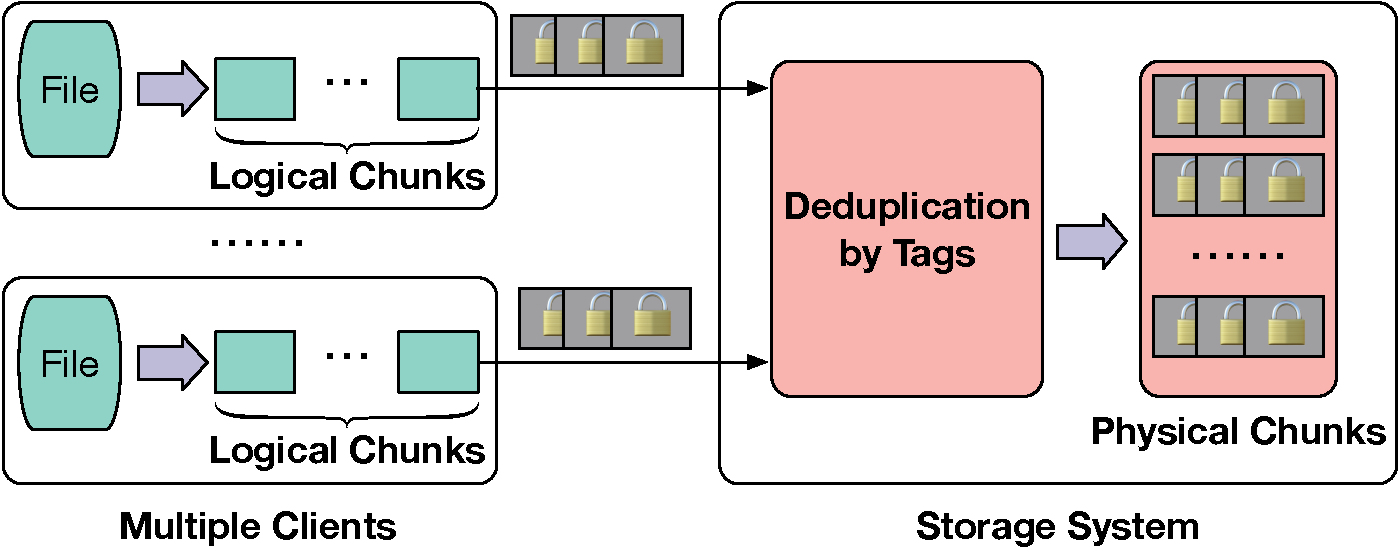
\includegraphics[width=.48\textwidth]{pic/dedup-view.pdf}
\caption{Overview of  deduplication workflow.}
\label{fig:dedup-view}
\end{figure}

We focus on {\em chunk-based deduplication}, which operates at the granularity
of small-size data units called {\em chunks}.  Figure~\ref{fig:dedup-view}
summarizes the deduplication workflow.  Specifically, a storage system first
partitions a file (e.g., backup) of a client into {\em logical chunks} via
some {\em chunking} procedure, such that each logical chunk is uniquely
identified by the cryptographic hash of its content called a {\em tag} (a.k.a.
fingerprint).  Two logical chunks are said to be {\em identical} if they have
the same tag, while the likelihood that distinct logical chunks have the same
tag is practically negligible \cite{black06}.  The storage system stores only
a copy of identical logical chunks as a {\em physical chunk}, and each
identical logical chunk refers to the same physical chunk via small-size
references.  

Chunk-based deduplication is more fine-grained than whole-file deduplication,
and hence has higher storage efficiency in general.  We can further choose
either {\em fixed-size} or {\em variable-size} chunking for deduplication.
Fixed-size chunking partitions file data into equal-size (logical) chunks,
while variable-size chunking (a.k.a. content-defined chunking) often specifies
chunk boundaries in a content-dependent manner (e.g., via Rabin fingerprinting
\cite{rabin81}) and partitions file data into variable-size chunks.
Fixed-size chunking is simple and fast, while variable-size chunking maintains
storage efficiency in the face of content shifts since the majority of chunks
remain unchanged even the file has added or removed some content.
Variable-size chunking is often used in backup systems (e.g.,
\cite{zhu08,lillibridge09}), yet fixed-size chunking is shown to be effective
for some workloads (e.g., VM images \cite{jin09}).  Our work addresses both
fixed-size and variable-size chunking approaches.  

{\em Encrypted deduplication} addresses chunk confidentiality in an
outsourcing environment (e.g., cloud storage), while preserving deduplication
effectiveness.  Traditional symmetric encryption requires that multiple
clients encrypt their file data by their (distinct) secret keys, thereby
transforming identical chunks into distinct encrypted chunks that can no
longer be deduplicated.  {\em Message-locked encryption (MLE)}
\cite{bellare13a} formalizes encrypted deduplication.  The baseline MLE
instantiation derives a symmetric key (called the {\em MLE key}) based on the
content of each {\em plaintext} (e.g., a logical chunk in chunk-based
deduplication), and encrypts the plaintext using the MLE key to form a {\em
ciphertext} (e.g., an encrypted logical chunk).  Thus, MLE ensures that
identical plaintexts are encrypted to identical ciphertexts.  Finally, the
storage system derives the tag from each ciphertext and performs
deduplication.  

MLE can be realized as different instantiations (see Section~\ref{sec:related}). The
most popular one is convergent encryption (CE) \cite{douceur02}, which has
been implemented in a wide variety of storage systems (e.g., 
\cite{adya02,elephantdrive,mega,gnunet,freenet,cryptosphere,cox02,storer08,
anderson10}).  The main idea of CE is to derive the MLE key from the
cryptographic hash of the content of each plaintext.  Note that some MLE
instantiations \cite{bellare13a} allow identical plaintexts to be encrypted
into distinct ciphertexts.  Nevertheless, they ensure that the tags are still
derived from the plaintexts, so that they can perform deduplication by
checking the equality of tags. 

Existing MLE instantiations all build on the notion {\em deterministic
encryption} to ensure that the ciphertexts (or the tags) are deterministically
derived from the plaintexts, so as to preserve deduplication effectiveness as
opposed to traditional symmetric encryption.  While deterministic encryption
provides confidentiality guarantees, in this paper, we argue that such a
deterministic nature can be exploited by an adversary to infer the original
plaintext from a given ciphertext. 

%Today, MLE \cite{bellare13a} and its variants \cite{douceur02, bellare13a, bellare13b, li15} have been implemented in various practical systems \cite{cryptosphere,elephantdrive, mega, adya02,freenet, wilcox-ohearn08, gnunet,li15,anderson10,cox02, armknecht15, shah15, qin17}. 

% from these distinct ciphertext chunks, and cannot detect whether the original content underlying these ciphertext chunks are identical.  

% The server cannot detect whether the original content underlying these  ciphertext chunks are identical; otherwise it violates the security guarantee of symmetric encryption.  

% For security concerns, users want their data to be encrypted before outsourcing.  

% Figure~\ref{fig:dedup-view} presents an overview of {\em encrypted deduplication} \cite{bellare13a}, where multiple clients outsource data to a remote storage system that performs {\em deduplication} across  clients to save storage space. Specifically, each client first partitions file data into {\em logical chunks}, each of which is with either fixed or variable sizes. 
% Fixed-size chunking achieves high computational performance, while variable-size chunking defines chunk boundaries based on  content so as to be robust against content shift. 


% Then, the client protects each chunk via encryption. However, in traditional symmetric encryption, clients use their own (distinct) secret keys for encryption, and transform the same plaintext chunks to different ciphertext chunks. The storage system cannot detect whether the original content underlying these ciphertext chunks are identical; otherwise it violates the security guarantee of symmetric encryption. 

% % To save space, the storage system performs {\em deduplication} across all its users. 

% Specifically, if two users upload the same message $M$, the server can detect this and store only a single copy of $M$. We focus on {\em chunk-based deduplication}, which partitions file data into fixed-size or variable-size chunks. Specifically, fixed-size chunking achieves high computational performance, while variable-size chunking defines chunk boundaries by content so as to be robust against content shift. Then, it removes duplicates in the graularity of chunk. In this paper, we use the term ``message'' and ``chunk'' interchangeably to refer to the fine-grained data unit operated by deduplication.   

% Deduplication is a technique that reduces storage space by eliminating content redundancies. Figure~\ref{fig:dedup-view} presents the logical view of a deduplication-enabled storage system, which operates at the granularity of {\em chunk} and removes the chunks that have identical content with some already stored chunks. 
% Specifically, it first partitions file data into an ordered sequence of {\em logical chunks}, each of which is with either fixed or variable sizes. 
% Fixed-size chunking achieves high computational performance, while variable-size chunking defines chunk boundaries based on  content so as to be robust against content shift. Then, it only stores the chunks (called {\em physical chunks}) that have unique content, and refers other copies of a stored chunk via small-size references. 

% Encrypted deduplication aims to address the chunk-level confidentiality of deduplication in an outsourcing environment (e.g., cloud storage). Consider a scenario where multiple users outsource storage to a remote third-party cloud service, which apply deduplication across its users to save storage space. For security concerns, users want their data to be encrypted before outsourcing. However, in traditional symmetric encryption, users use their own (distinct) secret keys for encryption, and  transform the same plaintext chunks to different ciphertext chunks. The server cannot detect whether the original content underlying these  ciphertext chunks are identical; otherwise it violates the security guarantee of symmetric encryption. 


% {\em Message-locked encryption (MLE)} \cite{bellare13a} is a cryptographic primitive to achieve encrypted deduplication. It derives a symmetric key $K_M$ (called {\em MLE key}) based on the content of each message $M$ (e.g., $K_M$ is the cryptographic hash of $M$ \cite{douceur02}), and further uses the MLE key $K_M$ to encrypt $M$. This makes the ciphertext only depend on the plaintext, from which it is encrypted. The server can detect duplicates by checking the equality of ciphertexts (e.g., comparing their cryptographic hashes). Today, MLE \cite{bellare13a} and its variants \cite{douceur02, bellare13a, bellare13b, li15} have been implemented in various systems \cite{cryptosphere,elephantdrive, mega, adya02,freenet, wilcox-ohearn08, gnunet,li15,anderson10,cox02, armknecht15, shah15, qin17}  for encrypted deduplication. 
   
% Consider a scenario where multiple users outsource storage to a remote third-party cloud service. To save space, the cloud server performs {\em deduplication} across all its users. Specifically, if two users upload the same message $M$, the server can detect this and store only a single copy of $M$. We focus on {\em chunk-based deduplication}, which partitions file data into fixed-size or variable-size chunks. Specifically, fixed-size chunking achieves high computational performance, while variable-size chunking defines chunk boundaries by content so as to be robust against content shift. Then, it removes duplicates in the graularity of chunk. In this paper, we use the term ``message'' and ``chunk'' interchangeably to refer to the fine-grained data unit operated by deduplication.   

% that have the same fingerprint are {\em identical}, since the probability of fingerprint collision (i.e., different chunks lead to the same fingerprint) is negligible in practice \cite{black06}. A deduplication system stores only a single copy of identical chunks, while referring the other copies by small-size references.  

% It performs chunking to partition input data into fixed-size or variable-size chunks. Fixed-size chunking generates all chunks that have a uniform chunk size; on the other hand, variable-size chunking, configured by the maximum, average and minimum chunk sizes, defines the boundary of each chunk (e.g., via Rabin fingerprinting \cite{rabin81}) through matching a specific content pattern. This makes it robust against content shift.

% \subsection{Leakage Channels}
% \label{sec:leakage}

% MLE applies {\em deterministic encryption}, and exposes some information, called {\em leakage}, about plaintext chunks. The fundamental leakage is {\em chunk frequency}, which is the number of times that each plaintext chunk appears in the original file data. Although the frequency leakage has been acknowledged in prior works \cite{abadi13,bellare15,ritzdorf16,li17}, it is hard to be prevented, since this breaks the one-to-one mapping between plaintext and ciphertext chunks, and leads to the degradation of deduplication performance \cite{abadi13} or storage efficiency \cite{li17} (see \S\ref{sec:countermeasure}).   


% sacrifices security and exposes some information,  
% that has been . Specifically, MLE encrypts identical plaintext chunks into identical ciphertext chunks, and hence leaks  We  


% Additional leakages \cite{ritzdorf16, li17} have been explored due to the careless deployment of encrypted deduplication. First, some deduplication systems \cite{xia11,lillibridge09,zhu08} aim for high performance, and operate chunks in the same order that they appear in plaintext files; this exposes the {\em logical order}, based on which one can identify the position of each chunk in input files. Second, some practitioners \cite{douceur02, wilcox-ohearn08, bellare13b} avoid storage overhead, and do not pad ciphertext chunks with any additional data; this exposes the {\em chunk size}, since the ciphertext chunks have the same number of blocks with corresponding plaintext chunks.  

% The risks posed by the above leakage profiles have not been scrutinized except \cite{ritzdorf16, li17}, which build attacks to infer the plaintext contents of ciphertext chunks \cite{li17} or to guess if particular files have already been stored \cite{ritzdorf16}. On the other hand, it remains unexplored that what is the security implication of the inferred information. This paper presents a comprehensive study of the leakage of encrypted deduplication, and we seek to answer the following questions: {\em (i) how to enable primitives to infer plaintext contents in various leakage settings, and (ii) what is the concrete implication from the inferred contents?}     




% \subsection{Frequency Analysis}
% \label{sec:freqanalysis}

% {\em Frequency analysis} is a well-known cryptanalysis primitive that illustrates the weakness of deterministic encryption. Suppose an adversary has access to a target set of ciphertexts (that are encrypted by deterministic encryption) and an auxiliary set of plaintexts. To launch frequency analysis, it sorts ciphertexts and plaintexts by their frequencies, respectively, and relates each ciphertext with the plaintext that has the same frequency rank. 
% Prior works have exploited different leakage profiles (e.g., access pattern \cite{kellaris16, lacharite18, islam12, zhang16b}, numeric order \cite{grubbs17, bindschaedler17, durak16}, query pattern \cite{cash15}) to examine frequency analysis in various applications (e.g., database \cite{naveed15}, keyword search \cite{grubbs16,pouliot16}). This paper shows how to strengthen the effectiveness of frequency analysis with practical leakages in deduplication. 

%The locality-based attack \cite{li17} targets deduplication, and increases the coverage of inferred chunks with an additional leakage of logical order.  




% strengthened the effectiveness of frequency analysis in different applications with various leakages.    

% Frequency analysis has been applied in prior works \cite{grubbs17,bindschaedler17,zhang16b,grubbs16,kellaris16,pouliot16,durak16,naveed15,cash15,islam12,lacharite18} to construct inference attacks. Some attacks target structured relational data in database, by classical frequency analysis \cite{naveed15}, exploring correlations or orderings of table columns, . 

% % Naveed {\em et al.} \cite{naveed15} propose $l_p$-optimization that equivalents classical frequency analysis.   


%  studies the security of encrypted database, and reduces classical frequency analysis to  problem.  

% on rational data 

% They either 


% The effectiveness of frequency analysis depends on the correlation between the auxiliary set and the target set. It performs well, only when the frequency of ciphertext is correlated with that of the corresponding plaintext. In addition, some ciphertexts (resp. plaintexts) may have the same frequencies, and form {\em ties} during sorting. How to break ties affects the result of frequency analysis. 

% This paper aims to apply frequency analysis to explore the vulnerabilities of encrypted deduplication. Our focus is not to address how to obtain correlated plaintexts for inference attack. Instead, we develop strategies to break ties effectively, so as to demonstrate the severity of frequency analysis.


% comment on March 15
% Deduplication eliminates the redundant copies of identical {\em chunks} for storage efficiency. It performs chunking to partition input data into fixed-size or variable-size chunks. Fixed-size chunking generates all chunks that have a uniform chunk size; on the other hand, variable-size chunking, configured by the maximum, average and minimum chunk sizes, defines the boundary of each chunk (e.g., via Rabin fingerprinting \cite{rabin81}) through matching a specific content pattern. This makes it robust against content shift. Each chunk is identified based on the cryptographic hash (known as {\em fingerprint}) of the content of the chunk. We consider the chunks that have the same fingerprint are {\em identical}, since the probability of fingerprint collision (i.e., different chunks lead to the same fingerprint) is negligible in practice \cite{black06}. A deduplication system stores only a single copy of identical chunks, while referring the other copies by small-size references.  


% Encrypted deduplication ensures all chunks are encrypted {\em before} deduplication, while the redundant copies of original chunks can still be removed. An elegant approach of resolving this tension is {\em message-locked encryption (MLE)} \cite{bellare13a}, which encrypts each chunk with a key derived from the content of the chunk. This maps identical plaintext chunks to identical ciphertext chunks that can be detected by deduplication. Today, various systems \cite{cryptosphere,elephantdrive, mega, adya02,freenet, wilcox-ohearn08, gnunet,li15,anderson10,cox02, armknecht15, shah15, qin17} (see \S\ref{sec:related}) have applied MLE \cite{bellare13a} or its variants \cite{douceur02, bellare13b, li15} for encrypted deduplication in practice. 

% However, the practical encrypted deduplication systems expose some information, called {\em leakage}, about the original chunks. The fundamental leakage is {\em chunk frequency} that has been acknowledged in prior works \cite{abadi13,bellare15,ritzdorf16,li17}. Specifically, MLE encrypts identical plaintext chunks into identical ciphertext chunks, and hence leaks the number of times that each original chunk appears in the input data. We argue that it is hard to prevent the frequency leakage, since this breaks the one-to-one mapping of plaintext and ciphertext chunks and hence degrades deduplication performance \cite{abadi13} or storage efficiency \cite{li17}. 


% Additional leakages \cite{ritzdorf16, li17} have been explored due to careless deployment of encrypted deduplication. First, some deduplication systems \cite{zhu08, xia11} aim for high performance, and require to operate chunks in the same order that they appear in original files; this exposes the {\em logical order}, based on which one can identify the position of each chunk in input files. Second, some practitioners \cite{douceur02, wilcox-ohearn08, bellare13b} avoid storage overhead and do not pad ciphertext chunks with any additional data; this exposes the {\em chunk size}, as the ciphertext chunks should have the {\em same} number of blocks with the original plaintext chunks.  

% The risks posed by leakage have not been scrutinized except \cite{ritzdorf16, li17}, which build {\em attack primitives} to infer original plaintext chunks \cite{li17} or the existence of particular files \cite{ritzdorf16} against encrypted deduplication. It remains unexplored of how to launch practical attacks based on the inferred information. This paper presents a comprehensive study of the leakage of encrypted deduplication, and we seek to answer the following two questions: {\em (i) how to enable primitives to infer original contents in various leakage settings, and (ii) what is the concrete implication of the practical attack that builds on the inferred contents?}     



% The present paper studies the leakage of SE in order to understand its practical security. We consider a range of threats including IKK’s query-identification setting, and against various approaches to building SE.


% To this end, we pose the following question: how to enable secure and lightweight rekeying, while preserving the deduplication capability?




% the work of IKK. The current literature leaves a practitioner with few concrete recommendations for configuring and deploying SE. The risk is not merely abstract; several deployments of SE may be easily broken depending on how they are used.

% Prior works

% to our best knowledge, none of schemes/systems attempt to protect the processing order of chunks. For performance reasons, some deduplication systems (e.g., DDFS \cite{zhu08} and SiLo \cite{xia11}) even require to operate chunks in the same order that they appear in the original logical files. This exposes the {\em logical order}, based on which one can identify the position of each chunk in the input file. 
   

% In addition to the frequency leakage, practitioners configure and deploy encrypted deduplication carelessly, and possibly . 


% In the following, we discuss a variety of leakages observed in the state-of-the-art encrypted deduplication schemes/systems.   

% \begin{itemize}[leftmargin=10pt]
% \item \textbf{Frequency leakage:} 
% Encrypted deduplication schemes apply {\em deterministic encryption} (e.g., MLE), where identical plaintext chunks will be encrypted into identical ciphertext chunks. This leaks the {\em frequency information} (i.e., the number of times that the original chunk appears in the input data) of each chunk. The frequency leakage is fundamental to MLE, as it is hard to be prevented (otherwise, leading to significant degradation of deduplication performance \cite{abadi13} or storage efficiency \cite{li17}).  

% \item \textbf{Size leakage:} 
% To mitigate storage overhead, practitioners are suggested to implement chunk encryption without padding schemes \cite{ritzdorf16}. For example, Farsite \cite{douceur02}, Tahoe-LAFS \cite{wilcox-ohearn08} and DupLESS \cite{bellare13b} apply AES in counter mode, yet they do not pad ciphertext chunks with any additional data. This leaks the {\em chunk size information} \cite{ritzdorf16}, as the ciphertext chunks should have the {\em same} number of blocks with the original plaintext chunks.  
% The leakage is more severe for variable-size chunks, whose boundaries are identified (e.g., via Rabin fingerprinting \cite{rabin81}) by matching a specific content pattern. A variable-size ciphertext chunk leaks the information that only the last a few bytes (determined by a sliding window) of its original chunk are likely to match the public content pattern. Two ciphertext chunks with distinct sizes further expose the information that they are mapped from different plaintext chunks.     
	 
% \item \textbf{Order leakage:}
% Leakage occurs in deploying encrypted deduplication carelessly. \end{itemize}

 
% This paper studies the leakage of encrypted deduplication. We present a family of new inference attacks that exploit the exposed information to learn the original content of encrypted chunks.

\chapter{Threat Model}
\label{sec:threat}

In this section, we formulate the threat model for our proposed frequency
analysis attacks against encrypted deduplication.  

\section{Definitions}

We first provide the definitions for our threat model. We model a plain file
as an ordered list of $n$ {\em logical plaintexts} (i.e., logical chunks
before deduplication), denoted by $\mathbf{M} = \langle \hat{M}^{(1)},
\hat{M}^{(2)}, \ldots, \hat{M}^{(n)}\rangle$.  Each logical plaintext
$\hat{M}^{(i)}$ (where $1\le i\le n$) is encrypted via MLE into the
corresponding ciphertext $\hat{C}^{(i)}$, and all encrypted results of
$\mathbf{M}$ form a stream of $n$ {\em logical ciphertexts} $\mathbf{C} =
\langle \hat{C}^{(1)}, \hat{C}^{(2)}, \ldots, \hat{C}^{(n)} \rangle$.  Note
that the logical ciphertexts in $\mathbf{C}$ are also ordered to reflect the
deduplication processing sequence of an encrypted deduplication storage
system.  

Identical logical plaintexts and ciphertexts may appear at different positions
of $\mathbf{M}$ and $\mathbf{C}$, respectively.  We denote a unique plaintext
as $M$ (uniquely identified by its tag), which is encrypted via MLE to the
corresponding unique ciphertext $C$.  Each $M$ (resp. $C$) corresponds to one
or multiple identical copies of $\hat{M}^{(i)}$ (resp. $\hat{C}^{(i)}$).  

% of $\mathbf{M}$ is
% independently encrypted into corresponding ciphertext $C$ via MLE, and all encrypted results     

% A unique plaintext (or plaintext for short) $M$ has one or more copies in $\mathbf{M}$  
% Identical plaintexts may have multiple copies in $\mathbf{M}$, and we introduce unique plaintext  
% We define a unique plaintext as the plaintext that has unique content among other plaintexts of $\mathbf{M}$    
% Let $M$ and $C$ be a
% plaintext and its corresponding ciphertext, respectively; both of them are in
% units of chunks defined by deduplication.  We model a plain file before
% deduplication as an {\em ordered} list of $n$ plaintexts, denoted by
% $\mathbf{M} = \langle M^{(1)},  M^{(2)}, \ldots, M^{(n)}\rangle$.  Identical
% plaintexts may appear at different positions of $\mathbf{M}$, say $M^{(i)} =
% M^{(j)}$ for some $1\le i \neq j\le n$.   
% % Also, each plaintext can have the
% same or different chunk sizes due to fixed-size or variable-size chunking,
% respectively, and let $|M|$ denote the size of a plaintext $M$.  
% Let $M$ and $C$ denote a
% plaintext (i.e., a logical chunk before encryption) and its corresponding
% ciphertext (i.e., a logical chunk after encryption).  We model a plain file

\section{Adversarial Goals and Assumptions}
\label{sec:assumptions}

We consider an adversary that aims to infer a set of ciphertext-plaintext
pairs, denoted by \{$(C, M)$\}, with two specific goals:
\begin{itemize}[leftmargin=*]
\item
{\bf High inference rate:} A large fraction of correct ciphertext-plaintext pairs
are inferred, among all correct ciphertext-plaintext pairs (i.e., high recall or
low false negative rates in statistical terms).
\item
{\bf High inference precision:} A large fraction of ciphertext-plaintext pairs
are correct, among all inferred ciphertext-plaintext pairs (i.e., high precision
or low false positive rates in statistical terms).
\end{itemize}
  
We assume that the adversary is {\em honest-but-curious}, such that it can
passively monitor the stream of ciphertexts $\mathbf{C}$ being written to the
storage system and exploit different types of leakage information from
$\mathbf{C}$ (see Section~\ref{sec:leakage}).  Given the available leakage
information, the adversary aims to infer the original plaintext of each
ciphertext in $\mathbf{C}$ via a {\em ciphertext-only} attack.  It is possible
that the adversary knows a limited subset of ciphertext-plaintext pairs to
launch a known-plaintext attack, which further strengthens attack severity
\cite{li17}.  We do not consider the known-plaintext attack in this paper. 

%We treat $\mathbf{C}$ as the {\em view} by the
%adversary and model different properties of the view 

We assume that the adversary does not have access to any {\em metadata} that
contains the information about how chunks are operated and stored, as we do
not apply deduplication to the metadata and hence it can be protected by
traditional symmetric encryption.  Also, we assume that the adversary does not
have {\em active} capabilities, which can be independently prevented by
existing approaches. One example is that a malicious client may claim the
ownership of unauthorized files in client-side deduplication
\cite{harnik10,halevi11,mulazzani11}; it can be addressed by
proof-of-ownership \cite{halevi11,xu13,pietro12} or server-side deduplication
\cite{harnik10,li15}.  Another example is that a malicious storage system may
modify stored data; it can be detected by remote integrity checking
\cite{juels07,ateniese07}. 

% In addition, $\mathcal{A}$ does not aim to infer if
% particular files have been stored \cite{harnik10, ritzdorf16}. Instead, we
% study the security implication based on the inferred contents over different
% types of files (see \S\ref{sec:case}).. 
% Intuitively, we want to guarantee that what $\mathcal{A}$ can learn is some
% well defined leakage $\mathcal{L}$, which includes the frequency, logical
% order and/or chunk size (\S\ref{sec:leakage}). 
% Note that $\mathcal{A}$ is specific to a {\em passive} adversary with content
% inference in mind. We do not assume $\mathcal{A}$ has {\em active}
% capabilities,   

\section{Leakage Channels}
\label{sec:leakage}

We consider three types of leakage channels in encrypted deduplication storage
that enable an adversary to infer information:
\begin{itemize}[leftmargin=*]
\item
{\bf Frequency:}  Due to the deterministic nature of encrypted deduplication,
the frequency of each ciphertext in $\mathbf{C}$ before deduplication (i.e., 
the number of duplicate copies) can be mapped to that of its corresponding
plaintext in $\mathbf{M}$. 
% the size of each ciphertext in
% $\mathbf{C}$ is approximately equal to that of its corresponding plaintext in
% $\mathbf{M}$. In other words, the exact number of blocks (e.g., that are of size 16 bytes) in ciphertexts   
% the exact number of blocks in the plaintext equals the number of blocks in the ciphertext
% {\bf PC: if block cipher is used, it's not necessary that the
% plaintext has the same size as its ciphertext}.
%(e.g., \cite{douceur02, wilcox-ohearn08, bellare13b}) do not pad ciphertexts
%with additional data to avoid storage overhead, 
\item
{\bf Order:}  Some storage systems (e.g., \cite{xia11,lillibridge09,zhu08})
apply deduplication to the chunks in the same order as they appear in the
original file.  Thus, the order of ciphertexts in $\mathbf{C}$ can be mapped
to that of plaintexts in $\mathbf{M}$. 
\item
{\bf Size:}  Variable-size chunking (see Section~\ref{sec:background}) leads
to different chunk sizes of the ciphertexts.  If such ciphertexts are not
padded (to avoid storage overhead \cite{ritzdorf16}), the size of a ciphertext
in $\mathbf{C}$ can be mapped to that of its corresponding plaintext in
$\mathbf{M}$.    
\end{itemize}

%We also consider other leakage channels that are specific to real-world
%deduplication storage systems. First, {\em order leakage} exposes the logical
%order of each plaintext, and it is available for the systems
%\cite{xia11,lillibridge09,zhu08} that aim for high performance and operate
%the deduplication of chunks in the same order as these chunks appear in
%original files; this implies that the logical order of ciphertext in
%$\mathbf{C}$ exactly reflects that of its corresponding plaintext. Second,
%{\em size leakage} exposes the chunk size of each plaintext, since some
%systems \cite{douceur02, wilcox-ohearn08, bellare13b} avoid storage
%overhead and do not pad ciphertexts with any additional data; this
%implies that the size of ciphertext in $\mathbf{C}$ exactly equals that
%of its corresponding plaintext.

In addition, the adversary has access to some {\em auxiliary information} that
presents the ground truth about the data characteristics correlated with
$\mathbf{M}$. Note that the availability of auxiliary information is necessary
for any inference attack \cite{kumar07,li17,grubbs17,zhang16b,kellaris16,ritzdorf16,naveed15,cash15,islam12}.
In this work, we consider the auxiliary information as an ordered list of
previously known plaintexts (e.g., old user backups or VM disk images),
denoted by $\mathbf{A}$.  Clearly, the attack severity depends on the
correlation between $\mathbf{A}$ (i.e., the previously known plaintexts) and
$\mathbf{M}$ (i.e., the plaintexts that are to be inferred).  Our focus is not
to address how an adversary can obtain auxiliary information, possibly due to
careless data release \cite{careless-release}, stolen storage devices
\cite{stolen-device}, and cloud leakage \cite{cloud-leakage}. Instead, given
such information, we investigate how the available auxiliary information,
combined with the leakage channels, bring information leakage from encrypted
deduplication. 

We focus on frequency analysis \cite{alkadit92} as the attack methodology.
Classical frequency analysis sorts the unique ciphertexts in $\mathbf{C}$ and
the unique plaintexts in $\mathbf{A}$ by {\em frequency} (i.e., the number of
identical copies corresponding to each unique ciphertext or unique plaintext). 
It then relates each unique ciphertext in $\mathbf{C}$ with the unique
plaintext in $\mathbf{A}$ that has the same frequency rank. In the following
sections, we design sophisticated frequency analysis attacks against encrypted
deduplication. 


% Frequency analysis is a cryptanalysis primitive to relate the ciphertexts in $\mathbf{C}$  with the plaintexts in $\mathbf{M}$. Specifically, it sorts ciphertexts and plaintexts by their frequencies in $\mathbf{C}$ and $\mathbf{A}$, respectively, and maps each ciphertext to the plaintext that has the same frequency rank. Building on the classical version of frequency analysis, we show how to exploit leakage channels to strengthen its severity against encrypted deduplication. 


% infer ciphertext-plaintext pairs from $\mathbf{C}$ and $\mathbf{A}$. 
 % Specifically, the adversary 

% It performs well, only when the frequency of ciphertext is correlated with that of the corresponding plaintext. 
% The more correlated to $\mathbf{M}$,  

% Our focus is not to address its availability, which is due to careless data release \cite{careless-release}, stolen storage devices \cite{stolen-device}, and cloud leakage \cite{cloud-leakage}. Instead, we show how an adversary can launch inference attacks based on the available auxiliary information $\mathbf{A}$. 

% Our focus is not to address how to obtain accurate auxiliary information, which we pose as future work; instead, given the available auxiliary information, we study how an adversary can design a severe attack based on frequency analysis and how we can defend against the attack
% Some available auxiliary information has been demonstrated to be necessary for inference attacks  and we consider the auxiliary information $\mathbf{M}$ as a complete user backup, file system snapshot or VM disk image in plaintext. The rationale of its availability is that the adversary can obtain the original data from  We emphasize that the auxiliary information $\mathbf{M}$ does not need to be identical with the original file of $\mathbf{C}$. In other words, $\mathbf{M}$ may not have the
% same number of chunks with $\mathbf{C}$, or its $i$-th chunk $M^{\langle i \rangle}$ may not be the plaintext of $C^{\langle i \rangle}$ or even not mapped into $\mathbf{C}$. 
% {\bf PC: give the background on frequency analysis.}




% We assume that the adversary can take advantage of some   for attacks. The auxiliary information , and it has been demonstrated for necessity in inference attacks . In this work,  

% In addition, the adversary can exploit other deduplication-specific leakage channels.

% effectiveness of inference attacks. First, we consider {\em size leakage}, meaning that the adversary can derive the size of a plaintext directly based on the corresponding ciphertext: ${\sf s}(C) = |M|$, where $C$ is the encryption of $M$.   

% deduplication-specific leakage channels.

% We target inference attacks against {\em backup workloads}, which refer to the copies of primary data (e.g., application states, file systems, and virtual disk images) over time. The recent technology trend \cite{douglis17} suggests to create full backups (that store the complete data of the primary source) over traditional incremental backups (that only store the changes of data since the last full backup), so as to mitigate the overhead in restoring earlier (full) backups. Thus, we focus on inferring information from different versions of full backups (or backups for short) that are created based on the same primary data source at different times.   

% They can be created as either weekly full backups (that store the complete data of the primary source) or daily incremental backups (that only store the changes of data since the prior full backup). Informed by the technology trend , we focus on full backups (or {\em backups} for short). Specifically, we aim to infer information from different versions of backups that are created based on the same primary data source yet at different times.    

% To launch attacks, we assume that $\mathcal{A}$ is an ``{\em honest-but-curious}'' adversary that can compromise the server hosting deduplication service, while it cannot establish a long-term presence for attack. Intuitively, we want to guarantee that what $\mathcal{A}$ can learn is some well defined leakage $\mathcal{L}$, which includes the frequency, logical order and/or chunk size (\S\ref{sec:leakage}). Formally, we define these leakage channels based on a target victim file $\mathbf{M}_{\rm t}$:

% \begin{itemize}[leftmargin=*]
% 	\item  {\bf Frequency leakage}: $\mathcal{L}_{\rm freq} = \{(C, {\sf freq}(M)): M \in \mathbf{M}_{\rm t}$ and $C = {\sf E}_{K_M}(M) \}$ is a set of chunk-frequency pairs, where $C$ is the encryption of some plaintext chunk $M$ in $\mathbf{M}_{\rm t}$, and each pair $(C, {\sf freq}(M))$ leaks the corresponding frequency of $M$. 

% 	\item  {\bf Order leakage}: $\mathcal{L}_{\rm order} = \{(C, {\sf ord}(M)): M\in\mathbf{M}_{\rm t}$ and $C = {\sf E}_{K_M}(M) \}$ associates each ciphertext chunk $C$ with a set ${\sf ord}(M)$ of logical orders, at which the copies of its original chunk $M$ appear in $\mathbf{M}_{\rm t}$. Note that order leakage {\em implies} frequency leakage, since the logical orders of each chunk copy inherently includes the number of times the corresponding chunk appears.    

% 	\item  {\bf Size leakage}: $\mathcal{L}_{\rm size} = \{(C, {\sf size}(M)): M \in \mathbf{M}_{\rm t}$ and $C = {\sf E}_{K_M}(M) \}$ is a set of chunk-size pairs, where each pair leaks the size of the original chunk of $C$.
% \end{itemize}

% In addition, $\mathcal{A}$ can take advantage of the {\em auxiliary information} $\mathbf{M}_{\rm a}$ that presents the ground truth about the frequency, size and order information about plaintext chunks. Some available auxiliary information is necessary for inference attacks , and we focus on validating our attacks with the auxiliary information obtained from different types of storage workloads (see \S\ref{sec:dataset}). 

% Acquiring the above capabilities, $\mathcal{A}$'s primary goal is to recover the plaintext chunks in the target file $\mathbf{M}_{\rm t}$. More formally, given the leakage $\mathcal{L}$ (that can be some combination of $\mathcal{L}_{\rm freq}$, $\mathcal{L}_{\rm order}$ and $\mathcal{L}_{\rm size}$) and the auxiliary information $\mathbf{M}_{\rm a}$, $\mathcal{A}$ outputs a collection of ciphertext-plaintext chunk pairs $\mathcal{R} = \{ (C, M) \}$: $\mathcal{A}(\mathcal{L}, \mathbf{M}_{\rm a}) \rightarrow \mathcal{R}.$ Each output pair $(C, M)$ indicates $\mathcal{A}$'s guess that relates a ciphertext chunk $C$ with a plaintext chunk $M$. 

% identify the ciphertext-plaintext chunk pairs about $\mathbf{M}_{\rm tar}$. More formally, given the leakage $\mathcal{L}$ (that can be some combinations of $\mathcal{L}_{\rm freq}$, $\mathcal{L}_{\rm order}$ and $\mathcal{L}_{\rm size}$), and auxiliary information $\mathbf{M}_{\rm aux}$, $\mathcal{A}$ outputs a collection of ciphertext-plaintext chunk pairs $\mathcal{R} = \{ (C, M) \}$: $\mathcal{A}(\mathcal{L}, \mathbf{M}_{\rm aux}) \rightarrow \mathcal{R}.$ Each pair $(C, M)$ indicates $\mathcal{A}$'s guess that relates a ciphertext chunk $C$ with a plaintext chunk $M$. 


% a malicious server may corrupt stored chunks, yet it can be detected by integrity checking mechanisms \cite{juels07,ateniese07};  

% and it is a correct inference by $\mathcal{A}$ if $C$ is the actual encryption of $M$, i.e., $(M, C) \in \mathcal{E}$.


% We measure the success of attacks in several ways. The {\em raw inference rate} is the percentage of ciphertext chunks (including duplicates) that are inferred correctly over the total number of ciphertext chunks in the target information. For example, if the adversary correctly infers a ciphertext-plaintext chunk pair $(C, M)$ and the ciphertext chunk $C$ accounts for a fraction of 10\% in the target information, then the raw inference rate will be at least 10\%. 


% We assume the adversary can eavesdrop the deduplication processing (e.g., comparison operation of fingerprints) of all ciphertext chunks in a victim file (called {\em target information}); on the other hand, it cannot access related metadata that can be protected by traditional encryption \cite{li17}. 
% the same and different private sources, as well as some public source .    

% Note that $\mathcal{A}$ is specific to a passive adversary with content recovery in mind. We do not abstract $\mathcal{A}$ with active capabilities, since these threats can be protected by existing approaches. For example, a malicious server may corrupt stored chunks, yet it can be detected by integrity checking mechanisms \cite{juels07,ateniese07}; a malicious client may cheat owning a particular file \cite{harnik10,halevi11,mulazzani11}, yet it can be addressed by proof of ownership \cite{halevi11} or enforcing server-side deduplication \cite{li15}. 


\chapter{Distribution-based Attack}
\label{sec:distribution-attack}

The distribution-based attack exploits the order information of $\mathbf{C}$
and $\mathbf{A}$ to strengthen the effectiveness of frequency analysis.  It
then compares the relative frequency distributions of $\mathbf{C}$ and
$\mathbf{A}$ to reduce the false positive results.  We also show how to
exploit chunk size information to further improve the inference precision.  

\section{Background: Locality-based Attack}
\label{sec:prior-attack}

The distribution-based attack builds on the previously proposed {\em
locality-based attack} \cite{li17}, which shows how frequency analysis causes
information leakage in backup workloads.  The locality-based attack considers
{\em full backups} (or backups for short) that are created as the complete
copies of primary data (e.g., application states, file system snapshots, and
VM disk images) on a daily or weekly basis. It aims to infer the
ciphertext-plaintext pairs across different versions of backups.  It assumes
that the auxiliary information $\mathbf{A}$ is derived from some older
backups, and its goal is to infer the plaintexts of the latest backup (i.e.,
$\mathbf{M}$). 

The locality-based attack leverages the {\em locality} property
\cite{xia11,zhu08,lillibridge09}, which is a common phenomenon in practical
backup workloads. Specifically, the locality property states that neighboring
chunks tend to co-occur in the {\em same order} across different versions of
backups before deduplication. The main reason is that the updates to each
backup are often clustered in some small regions of chunks, while the
remaining large stretch of chunks appear unchanged or preserve the same order
across different versions of backups.  

Based on locality, the locality-based attack exploits the order information to
discover the neighboring information of ciphertexts and plaintexts.
Specifically, for a given unique ciphertext $C$, the attack first identifies
the set of all identical copies $\{\hat{C}^{(i)}\}$.  For each
$\hat{C}^{(i)}$, it considers the left and right {\em neighbors} of
$\hat{C}^{(i)}$, i.e., $\hat{C}^{(i-1)}$ and $\hat{C}^{(i+1)}$, respectively.
It extracts the sets of left and right neighbors into the associative arrays
$\mathbf{L_C}$ and $\mathbf{R_C}$, respectively.  The associative arrays store
the mappings of each unique ciphertext $C$ and its {\em co-occurrence
frequencies} with its left and right neighbors, respectively.   Similarly, the attack also constructs the
associative arrays $\mathbf{L_A}$ and $\mathbf{R_A}$ based on the order
information of $\mathbf{A}$. 

The locality-based attack then iterates frequency analysis through the
neighbors of each inferred ciphertext-plaintext pair.  It first applies
frequency analysis to infer a number (parameterized by $u$) of top-frequent
ciphertext-plaintext pairs \{$(C, M)$\} from $\mathbf{C}$ and $\mathbf{A}$.
The inferred results are likely to be {\em real} (i.e., the target ciphertext
is indeed mapped from the inferred plaintext), based on the observation that
the ranks of highly frequent chunks are stable across different versions of
backups.  For each inferred pair $(C, M)$, the attack finds their left and
right neighbors that have the most co-occurrence frequencies with $C$ and $M$,
respectively.  Due to locality, the left and right neighbors of $M$ are likely
to be the original plaintexts of the corresponding left and right neighbors of
$C$, respectively.  Thus, the attack also includes the top-frequent left
(resp. right) neighbors of $C$ and $M$ into the set of the resulting inferred
ciphertext-plaintext pairs.  Finally, the attack procedure iterates until the
neighbors of each inferred ciphertext-plaintext pair are examined. 

%It applies frequency analysis to infer new ciphertext-plaintext pairs that
%have the same co-occurrence frequency rank among corresponding neighbors. The
%rationale is the order of chunks is preserved by chunk locality, and the left
%and right neighbors of $M$ are likely to be the original plaintexts of the
%corresponding neighbors of $C$. Thus, the attack further iterates the same
%frequency analysis through the neighbors of these newly inferred
%ciphertext-plaintext pairs, so as to increase attack severity.    

%if $u$ is small. The rationale is the ranks of highly frequent chunks are
%stable across backups. On the other hand, a smaller $u$ degrades the coverage
%of inferred ciphertext-plaintext pairs, and we examine the impact of $u$ in
%Section~\ref{sec:experiment-distribution}. 

However, the locality-based attack has a major weakness that it  introduces
a high number of false positives (i.e., incorrect ciphertext-plaintext pairs).
Since the main idea of frequency analysis is to map ciphertexts to plaintexts
with the same frequency ranks, any disturbance to frequency ranking (e.g., 
the updates across backups) can lead to incorrect ciphertext-plaintext pairs,
which can in turn comprise the inference of their neighbors.  Although the
locality-based attack is shown to effectively infer a significant fraction of
real ciphertext-plaintext pairs,  the adversary has low confidence to tell
whether each inferred ciphertext-plaintext pair is real or a false positive.  

% For example, our evaluation shows although the locality-based attack can correctly infer 15.2\% of ciphertext-plaintext pairs in some case, the false positives take around 65.2\% in its inference results. In other words, the adversary has low confidence in identifying whether the inferred ciphertext-plaintext pairs are correct or not.  


% Our observation is frequency analysis essentially dominates the severity of the locality-based attack, yet it is {\em sensitive to frequency ranking}. Specifically, any disturbance (e.g., due to data updates or sorting the tied chunks that have the same frequency) to the frequency rank can greatly degrade the inference accuracy. These incorrectly inferred ciphertext-plaintext chunk pairs will compromise the iterations of their neighboring chunks (see above), and hence lead to low inference rate. 
% Although the authors \cite{li17} use a parameter (e.g., $u$, see above) to limit only a small number of top-frequent chunk pairs to be returned by frequency analysis, we find that the trick is not enough for {\em severe} inference attacks that demand high inference rate and accuracy.  In our experiments, we show the trick is not enough for severity and accuracy. A lower bound, although achieves high accuracy, potentially decreases the number of inferred ciphertext-plaintext chunk pairs. 

 % The adversary adds the newly inferred top-frequent chunk pairs into $\mathcal{G}$, and iterates until $\mathcal{G}$ is empty.
% We apply frequency analysis to find the most frequent ciphertext-plaintext chunk pairs from each of LC and LM, and similarly from RC and RM. In other words, we find the left and right neighboring chunks of C and M that have the most co-occurrences with C and M themselves, respectively.
% infer new ciphertext-plaintext pairs from the neighbors of $C$ and $M$. Specifically, it sorts the left and right neighbors of $C$ and $M$ based on their co-occurrence frequencies with $C$ and $M$, respectively, and infer    
% collects their left and right neighbors, and applies frequency analysis 
% applies    
% on frequency analysis as underlying primitive, and repeats it based on . Specifically,  The key idea behind the locality-based attack is to 
% the original plaintext of ciphertext   
% which  
% . Specifically, chunk locality states   
% to repeat frequency analysis.  To exploit chunk locality, the adversary first applies   
% To launch locality-based attack, the adversary first  

% and iterates it based on {\em chunk locality} , which specifies neighboring chunks tend to co-occur in the same order. Specifically, the adversary first applies frequency analysis to initialize an inferred set $\mathcal{G}$ with a configurable number (parameterized by $u$) of top-frequent ciphertext-plaintext chunk pairs. These inferred pairs can be considered correct with a high probability when $u$ is not much large (see \S\ref{sec:bucket_description}). In each iteration, the adversary picks one pair $(C, M)$ out of $\mathcal{G}$, and identifies the corresponding neighboring chunks $\mathbf{L}_\mathcal{C}[C]$, $\mathbf{R}_\mathcal{C}[C]$, $\mathbf{L}_\mathcal{M}[M]$ and $\mathbf{R}_\mathcal{M}[M]$ of $C$ and $M$. It applies frequency analysis on
% $\mathbf{L}_\mathcal{C}[C]$ and $\mathcal{L}_\mathcal{M}[M]$, as well as $\mathbf{R}_\mathcal{C}[C]$ and $\mathbf{R}_\mathcal{M}[M]$, according to their co-occurrence frequencies with $C$ and $M$. The rationale is the order of chunks is preserved due to locality, and the left and right neighbors of $M$ are likely to be the original chunks of the left and right neighbors of $C$. The adversary adds the newly inferred top-frequent chunk pairs into $\mathcal{G}$, and iterates until $\mathcal{G}$ is empty. 

% Recall that a ciphertext may repeat in $\mathbf{C}$, and it can be associated with more than one co-occurrences in $\mathbf{L_C}$ and $\mathbf{R_C}$, each of which stores the number of times it appears with its left and right neighbors.  
% co-occur with  left and right neighbors. 
% store the co-occurrences of left and right neighboring ciphertext in $\mathbf{C}$, respectively.   
% Specifically, for the $i$-th plaintext $M^{(i)}$ of $\mathbf{M}$, it considers the {\em left} and {\em right neighbor} of $M^{(i)}$ as  $M^{( i-1 )}$ and $M^{( i+1 )}$, which appear directly before and after $M^{( i )}$ in $\mathbf{M}$, respectively. It collects the ordering of $\mathbf{A}$ in the form of the associative arrays $\mathbf{L_A}$ and $\mathbf{R_A}$, which store the co-occurrences of neighboring plaintexts in $\mathbf{A}$. 

% The attack assumes the adversary's knowledge of order information is distributional, in the form of the associative arrays $\mathbf{L}_\mathcal{C}$ and $\mathbf{R}_\mathcal{C}$, which map each ciphertext chunk $C$ to its left and right neighboring chunks and corresponding co-occurrence frequencies with $C$. Note that this can be computed exactly if the adversary knows $\mathcal{L}_o$. The adversary can also extract similar arrays $\mathbf{L}_\mathcal{M}$ and $\mathbf{R}_\mathcal{M}$ from $\mathbf{M}_a$.
% propose the  that builds on  in backup workloads.
% In this section, we present the {\em distribution-based attack}, which is applicable for {\em both} fixed-size and variable-size chunks in backup data. Specifically, the distribution-based attack targets {\em full backups} (or backups for short) that are created as the complete copies of primary data (e.g., application states, file systems, and VM images) on a daily or a weekly basis, and it aims to infer the ciphertext-plaintext pairs across different versions (e.g., $\mathbf{M}$ and $\mathbf{C}$) of backups. The distribution-based attack exploits the order information, meaning that the logical orders of plaintexts in orginal file are reflected by the sequences of corresponding ciphertexts in $\mathbf{C}$ (see Section~\ref{sec:leakage}). 
% The distribution-based attack builds on {\em chunk locality} \cite{xia11,lillibridge09,zhu08, li17}, which defines the co-occurrence of neighboring chunks in backups. We follow the notations of \cite{li17} to capture chunk locality.  Based on the neighborhood relationship, we construct the associative arrays $\mathbf{L_M}$ and $\mathbf{R_M}$ to store the co-occurrences of neighboring plaintexts. Specifically, for the plaintexts of $M$ and $M'$,  $\mathbf{L_M}[M][M']$ and $\mathbf{R_M}[M][M']$ store the number of times that $M'$ is the left and right neighbor of $M$ in $\mathbf{M}$, respectively. We also build the associative arrays $\mathbf{L_C}$ and $\mathbf{R_C}$ to store the co-occurrences of
% neighboring ciphertexts in $\mathbf{C}$.   


\section{Description of Distribution-based Attack}
\label{sec:distribution-attack-description}

The distribution-based attack extends the locality-based attack \cite{li17} to
significantly remove false positives.  It leverages the locality property in
backup workloads as in the locality-based attack.  In addition, for each
unique ciphertext $C$ in $\mathbf{C}$, we measure its {\em relative frequency
distribution} based on its co-occurrence frequencies with its neighbors.
Similarly, we examine the relative frequency distribution of each unique
plaintext $M$ in $\mathbf{A}$.  Our observation is that for a real
ciphertext-plaintext pair $(C, M)$, both $C$ and $M$ should have similar
relative frequency distributions; i.e., their co-occurrence frequencies with
their respective neighbors are similar.  We treat this observation as a more
general notion of the locality property, and use it as a condition to filter
possibly incorrect ciphertext-plaintext pairs. 

%Our insight is if $M$ is the original plaintext of $C$, then the relative
%frequency distributions of $M$ and $C$ are likely to be {\em similar}. The
%rationale is  $\mathbf{A}$ and $\mathbf{C}$ are mapped from the same source,
%and hence share a large stretch of unchanged chunks that preserve
%relative frequency distributions. In other words, we extend frequency
%analysis, and filter the possibly flawed ciphertext-plaintext pairs $(C,
%M)$, in which the relative frequency distributions of $C$ and $M$
%are significantly different. This is expected to improve the precision of
%inference results. 
% infer the ciphertext-plaintext pair $(C, M)$ only when $C$ and $M$ have similar relative frequency distributions. Thus, we can filter the flawed inference pairs, in which the relative frequency distributions of the ciphertext and corresponding plaintext are likely to be significantly different.  

\begin{figure}[t]
\centering
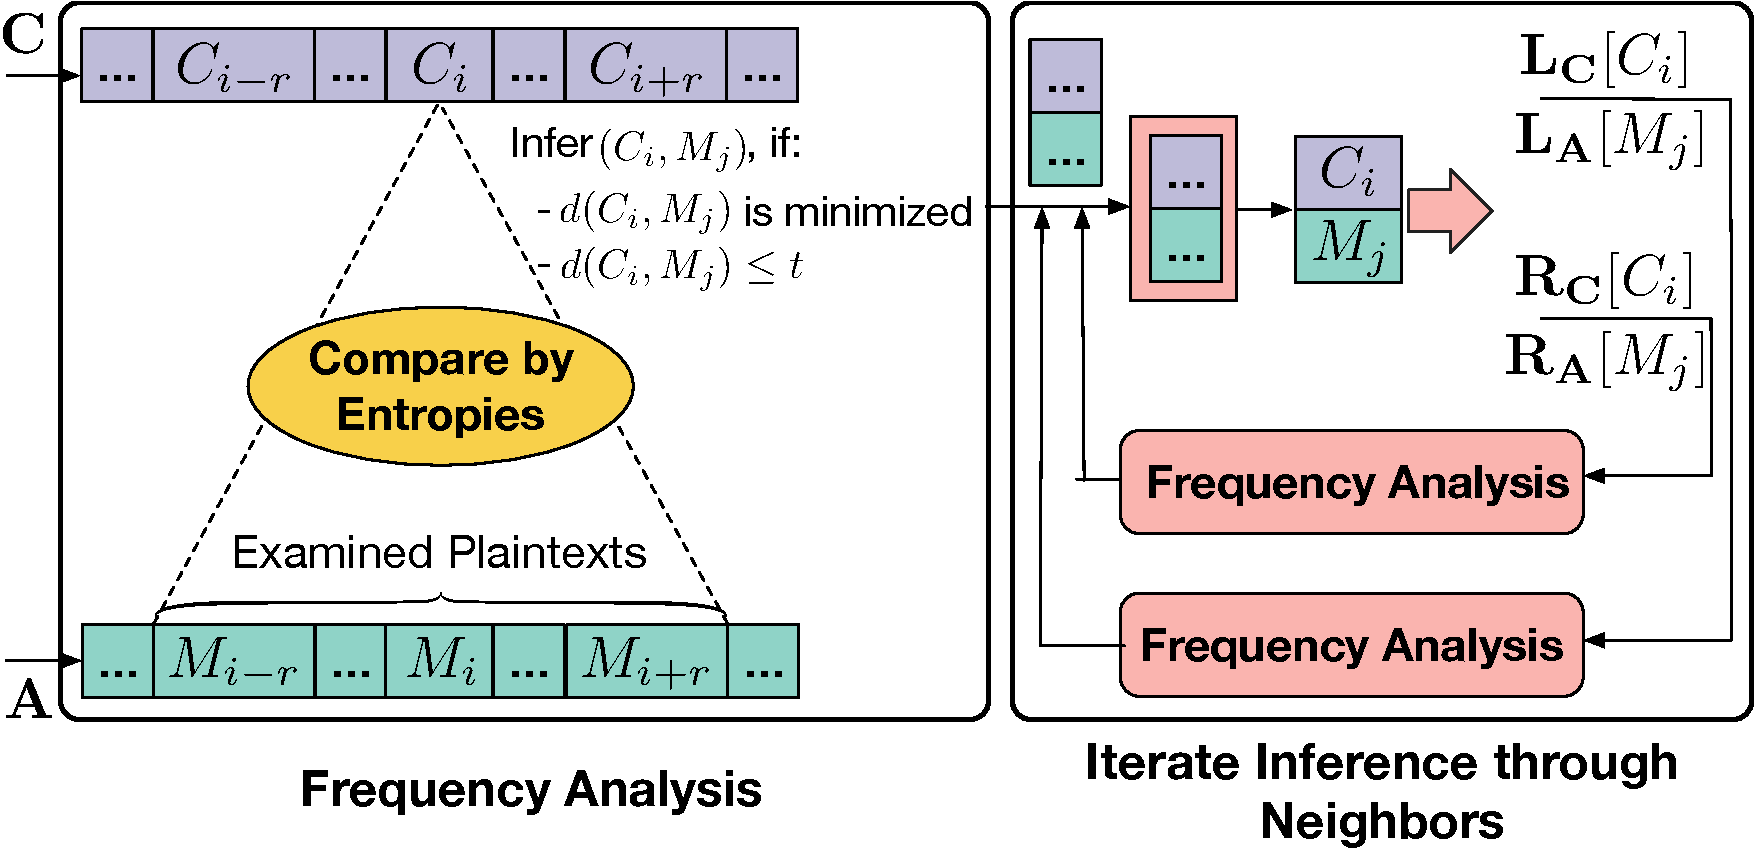
\includegraphics[width=.48\textwidth]{pic/distribution-attack.pdf}
\caption{Workflow of  distribution-based attack.}
\label{fig:distribution-attack}
\end{figure}

Figure \ref{fig:distribution-attack} presents the workflow of the
distribution-based attack. We first sort the unique ciphertexts and  plaintexts by
their frequencies in $\mathbf{C}$ and $\mathbf{A}$, respectively. As in the
locality-based attack \cite{li17}, we configure the parameter $u$ and 
the underlying frequency analysis to return at most $u$ ciphertext-plaintext
pairs.  In particular, for each unique ciphertext $C_i$ of rank $i$ (where 
$1 \leq i \leq u$), we examine a number of unique plaintexts $M_{i-r}, \ldots,
M_i, \ldots, M_{i+r}$ that rank from $i-r$ to $i+r$, where $r$ is a
configurable parameter (e.g., 10 by default) that indicates the maximum range
of rank disturbance that can be addressed. 

For each $C_i$ (where $1\le i\le u$) and the corresponding $M_j$ (where 
$i-r\le j\le i+r$),  we compare their relative frequency distributions by
{\em entropy}, a key concept in information theory that measures the amount of
information produced by a random source. Here, we adopt the entropy to 
{\em quantify the randomness of probability distribution} \cite{wang08}.
Specifically, we define two random variables, denoted by $X$ and $Y$, to
describe the co-occurrences of $C_i$ with its left and right neighbors,
respectively, such that the event ``$X=C$'' denotes the case that $C$ is the
left neighbor of $C_i$, and the event ``$Y=C$'' denotes the case that $C$ is
the right neighbor of $C_i$.  Thus, we compute the probabilities of both
events based on $\mathbf{L_C}$ and $\mathbf{R_C}$:   
%
\begin{eqnarray}
\Pr[X = C] = \frac{\mathbf{L_C}[C_i][C]}{\sum_{C' \in \mathbf{L_C}[C_i]} \mathbf{L_C}[C_i][C']}, \nonumber \\
\Pr[Y = C] = \frac{\mathbf{R_C}[C_i][C]}{\sum_{C' \in \mathbf{R_C}[C_i]} \mathbf{R_C}[C_i][C']}, \nonumber
\end{eqnarray}
%
where $\mathbf{L_C}[C_i]$ and $\mathbf{R_C}[C_i]$ store the left and right
neighbors of $C_i$, respectively, while $\mathbf{L_C}[C_i][C']$ and
$\mathbf{R_C}[C_i][C']$ store the co-occurrence frequencies of $C_i$ with its
left and right neighbor $C'$.  Both $X$ and $Y$ follow the relative frequency
distributions of $C_i$, and we characterize their randomness by entropies
denoted by $e(\mathbf{L_C}[C_i])$ and $e(\mathbf{R_C}[C_i])$, respectively:  
%
\begin{eqnarray}
    e(\mathbf{L_C}[C_i]) = \sum_{C \in \mathbf{L_C}[C_i]} \log_2\frac{1}{\Pr[X = C]}, \nonumber \\
    e(\mathbf{R_C}[C_i]) = \sum_{C \in \mathbf{R_C}[C_i]} \log_2\frac{1}{\Pr[Y = C]}. \nonumber
	% e_{C_i}.r = \sum_{C' \in \mathbf{R_C}[C_i]} {\sf log}_2 \frac{\mathbf{R_C}[C_i][C']}{\sum_{C'' \in \mathbf{R_C}[C_i]} \mathbf{R_C}[C_i][C'']}, 
\end{eqnarray}

Similarly, we compute the entropies $e(\mathbf{L_A}[M_j])$ and
$e(\mathbf{R_A}[M_j])$ of each $M_j$ based on $\mathbf{L_A}$ and
$\mathbf{R_A}$, respectively.  We then quantify the similarity of the relative
frequency distributions of $C_i$ and $M_j$ via the {\em Euclidean distance},
denoted by $d(C_i, M_j)$:  
% is used to measure the amount of information produced by a 
 % random source. Specifically, we compute the entropies $e_{C_i}.l$ and $e_{C_i}.r$ of $C_i$ based on the co-occurrence frequencies of $C_i$ with its left and right neighbors, respectively:  
% \begin{eqnarray}
	% e_{C_i}.l = \sum_{C' \in \mathbf{L_C}[C_i]} {\sf log}_2 \frac{\mathbf{L_C}[C_i][C']}{\sum_{C'' \in \mathbf{L_C}[C_i]} \mathbf{L_C}[C_i][C'']}, \\
	% e_{C_i}.r = \sum_{C' \in \mathbf{R_C}[C_i]} {\sf log}_2 \frac{\mathbf{R_C}[C_i][C']}{\sum_{C'' \in \mathbf{R_C}[C_i]} \mathbf{R_C}[C_i][C'']}, 
% \end{eqnarray}
% where $\mathbf{L_C}[C_i]$ and $\mathbf{R_C}[C_i]$ store the left and right neighbors of $C_i$, respectively, and $\mathbf{L_C}[C_i][C']$ and $\mathbf{R_C}[C_i][C']$ stores the co-occurrence frequencies of $C_i$ with its corresponding neighbor $C'$. Similarly, we compute the entropies $e_{M_j}.l$ and $e_{M_j}.r$ of each $M_j$ based on $\mathbf{L_M}$ and $\mathbf{R_M}$, and collectively measure the similarity of the relative frequency distributions of $C_i$ and $M_j$ via the Euclidean distance:  
\begin{eqnarray*}
	d(C_i, M_j) & = & 
	\big\{[e(\mathbf{L_C}[C_i]) - e(\mathbf{L_A}[M_j])]^2 \\
	& & + \ \ [e(\mathbf{R_C}[C_i]) - e(\mathbf{R_A}[M_j])]^2\big\}^{1/2}.
\end{eqnarray*}

Clearly, $C_i$ and $M_j$ have similar relative frequency distributions only
when the Euclidean distance $d(C_i, M_j)$ of their entropies is small.
Thus,  we identify $(C_i, M_j)$ as an inferred ciphertext-plaintext pair if
they satisfy the following requirements: 
%
\begin{itemize}[leftmargin=*]
\item {\bf R1:} $d(C_i, M_j)$ is the {\em smallest} for all $i-r \leq j \leq i+r$.
\item {\bf R2:} $d(C_i, M_j)$ is not larger than a pre-defined parameter $t$ (e.g., 1 by default).
\end{itemize}

% One special note is R1 is necessarily that some $M_j$  satisfies R1. 

One special note is that the original plaintext of $C_i$ may fall outside of
the examined plaintexts $M_{i-r}, \ldots, M_{i+r}$. 
In this case, R1 is still satisfied by some $M_j$ ($i-r \leq j \leq i+r$), and we expect to filter the incorrect ciphertext-plaintext pair by R2.     



% {\bf We use the requirement R2, and expect it can filter the flawed
% inference results that map $C_i$ to some $M_j$ in this case. PC: don't quite
% understand the statement???}

Then, we adopt the iteration paradigm in the prior locality-based attack \cite{li17} (see Section~\ref{sec:prior-attack}) to increase the coverage of inferred ciphertext-plaintext pairs. Specifically, for each inferred $(C_i, M_j)$, we apply the new frequency analysis scheme (see above) to infer more ciphertext-plaintext pairs through the neighbors of $C_i$ and $M_j$, and further iterate the same inference for those newly inferred pairs. We finally stop the iteration, when none of new ciphertext-plaintext pairs can be inferred.         

% Like the prior attack , we then iterate with each inferred  to infer more ciphertext-plaintext pairs from their neighbors. We apply the proposed new frequency analysis scheme (see above) through the left and right neighbors of $C_i$ and $M_j$, respectively, and      
% through the neighbors of  to infer more . , and further iterate   
% {\bf PC: can we not mention $\mathcal{Q}$ in this paragraph???} Then, we operate a first-in-first-out queue $\mathcal{Q}$, and apply the same locality-based paradigm (see Section~\ref{sec:prior-attack}) like the prior attack \cite{li17}. Specifically, we initialize $\mathcal{Q}$ with all ciphertext-plaintext pairs that have already been inferred. Each time, we pick one pair $(C_i, M_j)$ out of $\mathcal{Q}$, and apply the distribution-based frequency analysis (see above) over the left and right neighbors of $C_i$ and $M_j$, respectively. We include the newly inferred ciphertext-plaintext pairs into $\mathcal{Q}$, and finally stop the iteration until $\mathcal{Q}$ is empty.

 % For each inferred pair $(C_i, M_j)$, we apply the same locality-based paradigm like the prior attack \cite{li17}. Specifically, we operate a first-in-first-out queue $\mathcal{Q}$
% To repeat the distribution-based ranking, we initialize a first-in-first-out queue $\mathcal{Q}$ with the ciphertext-plaintext pairs inferred in Step 1. Each time, we pick one pair $(C_i, M_j)$ out of $\mathcal{Q}$, and apply the distribution-based ranking over their corresponding neighbors $\mathbf{L_C}[C_i]$ and $\mathbf{L_M}[M_j]$, as well as $\mathbf{R_C}[C_i]$ and $\mathbf{R_M}[M_j]$. From each case, we infer new ciphertext-plaintext pairs, and add them into $\mathcal{Q}$ for future loops. We finally stop the loop until $\mathcal{Q}$ is empty.
 % Our rationale of R2 is , and the parameter $t$ helps filter  
 % helps filter out these flawed inference results. 

\paragraph{Summary:} To summarize, the distribution-based attack provides a
more general notion of locality by considering the relative frequency
distribution during frequency analysis.  It is configured by three parameters
(i) $u$, which specifies the maximum number of ciphertext-plaintext pairs returned by frequency analysis, 
(ii) $r$, which specifies the maximum range of rank disturbance to be
considered, and (iii) $t$, which specifies the Euclidean distance threshold to
filter possibly incorrect inference results. 
The prior locality-based attack \cite{li17} can be regarded as a special case
of the distribution-based attack under the parameter configuration of $r = 0$
(i.e., without addressing any disturbance to frequency ranking) and 
$t\rightarrow\infty$ (i.e., without filtering any incorrect inference results).     
 
 % to 
 % specify the maximum range of disturbance to frequency ranking the scheme considers to address and the maximum entropy threshold  
 
 

% The locality-based attack can be regarded as a special case of the distribution-based attack under the  


\section{Exploiting Size Leakage}

We propose an advanced variant of the distribution-based attack that operates with size information to further reduce false positives. Specifically, we assume that the size of each ciphertext in $\mathbf{C}$ reflects that of its original plaintext.   

% The distribution-based attack addresses the precision of inference results by comparing relative frequency distributions. We argue that there is oppurtunity to further reduce the number of false positives by exploiting size leakage. Specifically, we make an additional assumption that  

% The rationale is symmetric encryption (e.g., block cipher) preserves the number of blocks.

Our idea builds on the fundamental truth that if a ciphertext $C$ corresponds to a plaintext $M$, then the size of $C$ approximates that of $M$. This is because encrypted deduplication preserves the number of blocks (i.e., the basic units operated by symmetric encryption) in the content to be encrypted. We use this fact to further filter the incorrect ciphertext-plaintext pairs $(C, M)$, where the number of blocks in $C$ and $M$ are different.  

% In other words, the number of blocks in each plaintext is exactly mapped to that in the corresponding ciphertext.     

% Our idea is based on the fundamental truth that if $C$ is mapped from $M$, then the size of $C$ approximates that of $M$. This is because encrypted deduplication preserves the number of blocks. In other words, we can filter the candiate pair $(C_i, M_j)$, where the number of blocks of $C_i$ and $M_j$ are different. 

In this work, we assume that each block is of 16 bytes, which is a typical configuration for AES. For each considered ciphertext-plaintext pair $(C_i, M_j)$, we derive the number of blocks in $C_i$ and $M_j$ as $b({C_i})$ and $b({M_j})$, respectively:
\begin{eqnarray*}
b({C_i}) = \lceil \frac{{\sf size}(C_i)}{16} \rceil, \nonumber \\
b({M_j}) = \lceil \frac{{\sf size}(M_j)}{16} \rceil, \nonumber 
\end{eqnarray*}
where ${\sf size}(C_i)$ and ${\sf size}(M_j)$ are the exact sizes of $C_i$ and $M_j$, respecitively, and $\lceil x \rceil$ returns the smallest integer greater than or equal to $x$. In addition to R1 and R2 (see Section~\ref{sec:distribution-attack-description}), we apply the following requirement to filter by size:    
\begin{itemize}[leftmargin=*]
    \item {\bf R3:} $b({C_i})$ equals $b({M_j})$.
\end{itemize}

The requirement R3 is effective to filter the incorrect ciphertext-plaintext pairs regarding variable-size chunks, where different chunks possibly have distinct sizes. However, for fixed-size chunks, it is always satisfied by the ciphertext-plaintext pairs, even they are incorret. Despite of this, we can still apply R1 and R2 to achieve high-precision attack.        



% for filtering false positives in terms of only variable-size chunks, where different chunks have possibly distinct sizes. On the other hand, it is always satisfied by fixed-size chunks, and cannot improve the precision of inference results in this case. Even so, we can still apply R1 and R2 to significantly reduce the amount of false positives in the locality-based attack \cite{li17} (see Section~\ref{sec:distribution-attack-description}).

% by {\bf about 50\%} (see Section~\ref{sec:experiment-distribution}). 

% percentage of false positives below 25\% .       

% \paragraph{Discussion:}
% The filtering effect of R3 depends on the size distribution of  (variable-size) chunks. Since encrypted deduplication only preserves approximate size (i.e., the number of blocks), R3 cannot detect the false positive, which maps a ciphertext to some flawed plaintext that shares the same number of blocks with corresponding exact plaintext. This makes it less effective in addressing inference precision against the workloads, where the sizes of majority chunks are clustered within a small range.   


% Specifically, it is less effective in reducing the number of false positives against the workloads, in which the sizes of chunks are clustered into a small range. The reason is the adversary who observes the size of a ciphertext can only deduce the number of blocks in corresponding plaintext.  


% The plaintexts whose sizes are clustered are more likely to have the same number of blocks, and the adversary cannot distinguish them by size.   


% The main reason is the adversary can deduce the size of the plaintext in the quantization factor of block size.   
% Due to the above facts, an adversary who can see the length of a ciphertext can readily deduce the length of the respective plaintext, except for a quantization factor of 8 or 128 respectively. The larger the quantization factor, the less resolution the attacker has regarding plaintext length information. Rupture is able to attack ciphers with even large quantization factors, yet a larger factor can make the attack slower. While the quantization factor can be made arbitrarily large when designing ciphers, the penalty being paid is in bandwidth consumed to transmit the ciphertext.
% and R3 is less effective in reducing the false positives against small-size chunks.
% only for variable-size chunks, where different chunks have possibly distinct sizes. It is naturally satisfied by fixed-size chunks, and cannot filter any false positives. In this case, this  
% In addition, the effect of R3 depends on the (average) size of chunks.  



% \paragraph{Discussion:}
% The size-based attack builds on the assumption of varying sizes of chunks, and demonstrates security alert only in variable-size chunking. In other words, the size-based attack will degrade to classical frequency analysis under fixed-size chunking, in which all plaintexts or ciphertexts have a uniform size and come into a single entry of the associative array.  
% The effectiveness of the size-based attack depends on the (average) size of chunks, and it is less effective for inferring small-size chunks. For example, we have evaluated that the size-based attack infers as low as 0.32\% of ciphertext-plaintext pairs against the chunks of an average size of 2KB (for comparison, it can infer up to 31.3\% ciphertext-plaintext pairs in our experiment of 8KB-size chunks, see Section~\ref{sec:experiment-size}). This is mainly for two reasons. First, small-size chunks are likely to have limited  variance on their size, and aggregate into a few entries of the associative array; this degrades the coverage of inferred pairs (recall that the attack  returns a limited number of ciphertext-plaintext pairs for each available chunk size). Second, each entry of the associative array is likely to include a large amount of small-size chunks, among which
% there tend to exist many ties where chunks have the same frequency; 
 % this possibly introduces additional false positives into frequency analysis \cite{naveed15, li17}. 




% For each $M_j$ ($i-r \leq j \leq i+r$), we compute similar entropies $e_{M_j}.l$ and $e_{M_j}.r$ for $M_j$, and collectively measure the similarity of the relative frequency distributions of $C_i$ and $M_j$ via the Euclidean distance:  

% We first sort available ciphertexts and plaintexts by their frequencies in $\mathbf{C}$ and $\mathbf{M}$, respectively. Next, we consider the distribution-based ranking scheme configured by a tuple of parameters $(u, r, t)$, in order to infer at most $u$ ciphertext-plaintext pairs. Specifically, for each ciphertext $C_i$ of rank $i$ ($1 \leq i \leq u$), we examine the plaintexts $M_{i-r},\ldots,M_i,\ldots,M_{i+r}$ that rank from $i-r$ to $i+r$, where $r$ (e.g., 10 by default) indicates the maximum range of rank disturbance can be addressed by the distribution-based ranking scheme. Then, we compute the entropies $e_{C_i}.l$ and $e_{C_i}.r$ of $C_i$ based on the co-occurrences of $C_i$ with its left and right neighbors, respectively:\footnote{Alternatively, we can calculate the entropies (that depend on the associative arrays $\mathbf{L_C}$ and $\mathbf{R_C}$) in
% pre-processing, rather than computing them on the fly.} 
% \begin{eqnarray}
% 	e_{C_i}.l = \sum_{C' \in \mathbf{L_C}[C_i]} {\sf log}_2 \frac{\mathbf{L_C}[C_i][C']}{\sum_{C'' \in \mathbf{L_C}[C_i]} \mathbf{L_C}[C_i][C'']}, \\
% 	e_{C_i}.r = \sum_{C' \in \mathbf{R_C}[C_i]} {\sf log}_2 \frac{\mathbf{R_C}[C_i][C']}{\sum_{C'' \in \mathbf{R_C}[C_i]} \mathbf{R_C}[C_i][C'']}, 
% \end{eqnarray}
% where $\mathbf{L_C}[C_i]$ and $\mathbf{R_C}[C_i]$) store the left and right neighbors of $C_i$, respectively, and $\mathbf{L_C}[C_i][C']$ and $\mathbf{R_C}[C_i][C']$ stores the co-occurrences of $C_i$ with its corresponding neighbor $C'$. For each $M_j$ ($i-r \leq j \leq i+r$), we compute similar entropies $e_{M_j}.l$ and $e_{M_j}.r$ for $M_j$, and collectively measure the similarity of the relative frequency distributions of $C_i$ and $M_j$ via the Euclidean distance:  
% \begin{eqnarray}
% 	{\sf Sim}(C_i, M_j) = \sqrt{(e_{C_i}.l - e_{M_j}.l)^2 + (e_{C_i}.r - e_{M_j}.r)^2}.  
% \end{eqnarray}

%  We infer $(C_i, M_j)$ as a ciphertext-plaintext pair, if (i) ${\sf Sim}(C_i, M_j)$ is the {\em smallest} among all examined plaintexts, and (ii) ${\sf Sim}(C_i, M_j)$ is not larger than the parameter $t$ (e.g., 1 by default). Our rationale is that the original plaintext of $C_i$ may fall outside of $M_{i-r}, \ldots, M_{i+r}$ (e.g., the range of rank disturbance is greater than $r$), and the pre-defined upper bound $t$ helps filter out these flawed inference results. 





% Our insight is that if $M$ is the underlying plaintext of $C$, then the relative frequency distributions of $C$ and $M$ are likely to be {\em similar}. The rationale is that $\mathbf{M}$ and $\mathbf{C}$ are from the same primary data (at different time), and hence share a large stretch of unchanged chunks due to chunk locality. Thus, we can adjust the ranking of classical frequency analysis by taking relative frequency distribution into consideration. Specifically, for each ciphertext $C_i$ of rank $i$ and plaintext $M_j$ of rank $j$, we compare their relative frequency distributions, say by the {\em entropies} on the co-occurrences of their neighbors. If they have similar entropy values, we say their relative frequency distributions are similar, and we call $(C_i, M_j)$ as an inferred ciphertext-plaintext pair, even though $C_i$ and $M_j$ have different ranks (i.e., $i \neq j$). 



% Thus, we can operate frequency analysis while taking relative frequency distribution into consideration, in order to filter out the inference results, in which the relative frequency distributions of the ciphertext and plaintext are significantly different. 
% Specifically, for each  plaintext $M$, we consider its {\em relative frequency distribution} that is counted by the co-occurrences of $M$ with its neighboring plaintexts (recall that $M$ may have duplicate copies and hence multiple neighbors in $\mathbf{M}$). We also count the relative frequency distribution of each ciphertext $C$.  
 % Thus, we can adjust the ranking of classical frequency analysis by taking relative frequency distribution into consideration. Specifically, for each ciphertext $C_i$ of rank $i$ and plaintext $M_j$ of rank $j$, we compare their relative frequency distributions, say by the {\em entropies} on the co-occurrences of their neighbors. If they have similar entropy values, we say their relative frequency distributions are similar, and we call $(C_i, M_j)$ as an inferred ciphertext-plaintext pair, even though $C_i$ and $M_j$ have different ranks (i.e., $i \neq j$). 
% The key idea of our attack is to inspect the distribution of , so as to filter out potentially flawed inference results.
% t further inspects the relative frequency distribution of the data and filters any potentially flawed inference results.
% We propose to extend chunk locality, and examine the frequency .  




% Inspired by chunk locality (see \S\ref{sec:locality}), we move one step further to examine the co-occurrence of neighboring chunks.
% Specifically, for each chunk, we consider its {\em relative frequency distribution} that is counted by the number of co-occurrences with its neighbors (recall that a chunk may have duplicate copies and hence multiple neighboring chunks). Our insight is that identical chunks likely have {\em similar} relative frequency distributions across backups. The rationale is updates to backups appear in few clustered regions of chunks, while the remaining majority regions of chunks preserve their co-occurrence relationships.


% Chunk locality states that neighboring chunks tend to co-occur under the same order across backups. For example, if a plaintext $M$ is surrounded by the plaintexts $M'$ and $M''$ in one backup, then $M$ is also likely to be surrounded by $M'$ and $M''$ in the following backups. Prior works \cite{xia11,lillibridge09,zhu08} have exploited chunk locality to improve performance, while we adapt it into addressing the false positives in frequency analysis. Specifically, classical frequency analysis is sensitive to frequency ranking, and any disturbances (e.g., due to data updates across backups or ranking the ciphertexts/plaintexts that have identical frequency) to the frequency ranking can introduce a significant amount of flawed inference results.  
   % In the following, we show how to build on chunk locality to construct an inference attack with low false positives. We first elaborate the key designs of the distribution-based attack, and then present the attack details step by step. 


% {\bf say drawback of classical frequency analysis}   

   


% Take {\em backups}, the complete copies of some primary data (e.g., application states, file systems, and VM images), as an example, if a plaintext $M$ is surrounded by the plaintexts $M'$ and $M''$ in one backup, then $M$ is also likely to be surrounded by $M'$ and $M''$ in the following backup from the same primary data. Prior works \cite{xia11,lillibridge09,zhu08} have exploited chunk locality to improve performance, while we adapt it into addressing the false positives of inference attack.   

% Figure \ref{fig:distribution-attack} shows an overview of the distribution-based attack. Given the input of $\mathbf{M}$ and $\mathbf{C}$, it builds on the {\em distribution-based ranking} to reduce the number of false positives in classical frequency analysis. Specifically, for each  plaintext $M$, we consider its {\em relative frequency distribution} that is counted by the co-occurrences of $M$ with its neighboring plaintexts (recall that $M$ may have duplicate copies and hence multiple neighbors in $\mathbf{M}$). We also count the relative frequency distribution of each ciphertext $C$.  
% Our insight is that if $M$ is the underlying plaintext of $C$, then the relative frequency distributions of $C$ and $M$ are likely to be {\em similar}. The rationale is that $\mathbf{M}$ and $\mathbf{C}$ are from the same primary data (at different time), and hence share a large stretch of unchanged chunks due to chunk locality. Thus, we can adjust the ranking of classical frequency analysis by taking relative frequency distribution into consideration. Specifically, for each ciphertext $C_i$ of rank $i$ and plaintext $M_j$ of rank $j$, we compare their relative frequency distributions, say by the {\em entropies} on the co-occurrences of their neighbors. If they have similar entropy values, we say their relative frequency distributions are similar, and we call $(C_i, M_j)$ as an inferred ciphertext-plaintext pair, even though $C_i$ and $M_j$ have different ranks (i.e., $i \neq j$). 

% For each inferred ciphertext-plaintext pair $(C_i, M_j)$, we repeat the same inference (see above) through their neighbors. Specifically, we collect the left and right neighbors of $C_i$,  as well as of $M_j$, respectively, and apply the distribution-based ranking over their corresponding neighbors, in order to infer new ciphertext-plaintext pairs. The rationale is that chunk locality preserves orders, and the left and right neighbors of $M_j$ are likely to be the underlying plaintexts of the left and right neighbors of $C_i$, respectively. We further repeat the inference through the neighbors of these newly inferred ciphertext-plaintext pairs, so as to increase the coverage of inferred pairs.  

% Then, we describe the details of the distribution-based attack.


% The distribution-based ranking proceeds as follows. We first rank available ciphertexts and plaintexts by their frequencies in $\mathbf{C}$ and $\mathbf{M}$, respectively. 
% Thus, we can adjust the ranking of classical frequency analysis by taking the relative frequency distribution of each plaintext and ciphertext into account. In other words, suppose $C_i$ and $M_j$ are the $i$-th and $j$-th top frequent ciphertext and plaintext, respectively.  
% This allows to infer the ciphertext-plaintext pair like $(C_i, M_j)$ 
% To perform distribution-based ranking, 



% Thus, we          
% Thus, we first establish the frequency-only ranking like classical frequency analysis (see \S\ref{sec:freqanalysis}), and then adjust the ranking by taking into account the relative frequency distributions of chunks. Roughly, we break rank disturbances and infer the ciphertext-plaintext chunks pairs
% $(C_i, M_j)$, where $C_i$ and $M_j$ have similar relative frequency distribution yet possibly different ranks (e.g., $i \neq j$). We refer the Step 1 of the attack for detailed requirements of $C_i$ and $M_j$.  



% We propose a new (frequency-based) ranking primitive, named {\em distribution-based ranking}, to address the ties incurred in classcial frequency analysis (see \S\ref{sec:freqanalysis}). Specifically, for each chunk, we consider its {\em relative frequency distribution} that is counted by the co-occurrences with its neighbors (recall that a chunk may have duplicate copies and hence multiple neighbors). Our insight is that the relative frequency distribution of the same chunk must be similar across backups. The reason is chunk locality implies that the majority stretches of chunks are unchanged. Thus, we first establish the frequency-only ranking like classical frequency analysis (see \S\ref{sec:freqanalysis}), and then adjust the ranking by taking into account the relative frequency distributions of chunks. Roughly, we break rank disturbances and infer the ciphertext-plaintext chunks pairs
% $(C_i, M_j)$, where $C_i$ and $M_j$ have similar relative frequency distribution yet possibly different ranks (e.g., $i \neq j$). We refer the Step 1 of the attack for detailed requirements of $C_i$ and $M_j$.  
% We elaborate the details below.

% \paragraph{Step 1 (Distribution-based ranking):}
% We first sort available ciphertexts and plaintexts by their frequencies in $\mathbf{C}$ and $\mathbf{M}$, respectively. Next, we consider the distribution-based ranking scheme configured by a tuple of parameters $(u, r, t)$, in order to infer at most $u$ ciphertext-plaintext pairs. Specifically, for each ciphertext $C_i$ of rank $i$ ($1 \leq i \leq u$), we examine the plaintexts $M_{i-r},\ldots,M_i,\ldots,M_{i+r}$ that rank from $i-r$ to $i+r$, where $r$ (e.g., 10 by default) indicates the maximum range of rank disturbance can be addressed by the distribution-based ranking scheme. Then, we compute the entropies $e_{C_i}.l$ and $e_{C_i}.r$ of $C_i$ based on the co-occurrences of $C_i$ with its left and right neighbors, respectively:\footnote{Alternatively, we can calculate the entropies (that depend on the associative arrays $\mathbf{L_C}$ and $\mathbf{R_C}$) in
% pre-processing, rather than computing them on the fly.} 
% \begin{eqnarray}
% 	e_{C_i}.l = \sum_{C' \in \mathbf{L_C}[C_i]} {\sf log}_2 \frac{\mathbf{L_C}[C_i][C']}{\sum_{C'' \in \mathbf{L_C}[C_i]} \mathbf{L_C}[C_i][C'']}, \\
% 	e_{C_i}.r = \sum_{C' \in \mathbf{R_C}[C_i]} {\sf log}_2 \frac{\mathbf{R_C}[C_i][C']}{\sum_{C'' \in \mathbf{R_C}[C_i]} \mathbf{R_C}[C_i][C'']}, 
% \end{eqnarray}
% where $\mathbf{L_C}[C_i]$ and $\mathbf{R_C}[C_i]$) store the left and right neighbors of $C_i$, respectively, and $\mathbf{L_C}[C_i][C']$ and $\mathbf{R_C}[C_i][C']$ stores the co-occurrences of $C_i$ with its corresponding neighbor $C'$. For each $M_j$ ($i-r \leq j \leq i+r$), we compute similar entropies $e_{M_j}.l$ and $e_{M_j}.r$ for $M_j$, and collectively measure the similarity of the relative frequency distributions of $C_i$ and $M_j$ via the Euclidean distance:  
% \begin{eqnarray}
% 	{\sf Sim}(C_i, M_j) = \sqrt{(e_{C_i}.l - e_{M_j}.l)^2 + (e_{C_i}.r - e_{M_j}.r)^2}.  
% \end{eqnarray}

%  We infer $(C_i, M_j)$ as a ciphertext-plaintext pair, if (i) ${\sf Sim}(C_i, M_j)$ is the {\em smallest} among all examined plaintexts, and (ii) ${\sf Sim}(C_i, M_j)$ is not larger than the parameter $t$ (e.g., 1 by default). Our rationale is that the original plaintext of $C_i$ may fall outside of $M_{i-r}, \ldots, M_{i+r}$ (e.g., the range of rank disturbance is greater than $r$), and the pre-defined upper bound $t$ helps filter out these flawed inference results. 


% We  apply classical frequency analysis to establish the (frequency-only) ranking on the plaintext chunks in $\mathbf{M}_{\rm a}$, as well as on the ciphertext chunks in $\mathcal{L}_{\rm order}$. Like the size-based attack (see \S\ref{sec:size-attack-description}), we configure the parameter $u$ that indicates the {\em maximum} number of most frequent chunk pairs to be inferred by our distribution-based ranking scheme.  
% Then,  For $C_i$ and each $M_j$ $(i-r \leq j \leq i+r)$, we compare their relative frequency distributions, say by the {\em entropies} of neighboring chunks. Specifically, we compute the entropies $e_{M_j}.l$ and $e_{M_j}.r$ based on the co-occurrences of $M_j$ and its left and right neighbors, respectively:    
% (recall that we can access the co-occurrences of $M_j$ and its neighbors from $\mathbf{L}_{\rm a}$ and $\mathbf{R}_{\rm a}$).    



% For example, if a chunk $M$ is surrounded by the chunks $M'$ and $M''$ in one backup, then $M$ is also likely to be surrounded by $M'$ and $M''$ in the following backups. The rationale is that the changes of backups often affect a few chunks, while the remaining chunks repeat in the same order. 

% The distribution-based attack builds on {\em chunk locality}  that is defined based on the neighborhood of chunks. Specifically, given a logical chunk $M^{\langle i \rangle}$, we define its {\em left} (resp. {\em right}) {\em neighbor} as the logical chunk $M^{\langle i-1 \rangle}$ (resp. $M^{\langle i+1 \rangle}$) that appears directly before (resp. after) $M^{\langle i \rangle}$. 

% To capture chunk locality, we build the associative arrays $\mathbf{L}_{\rm a}$ and $\mathbf{R}_{\rm a}$, which store the co-occurrences of neighboring  chunks in the auxiliary information $\mathbf{M}_{\rm a}$. Specifically, for two neighboring chunks $M$ and $M'$, $\mathbf{L}_{\rm a}[M][M']$ (resp. $\mathbf{R}_{\rm a}[M][M']$) stores the number of times that $M'$ is the left (resp. right) neighbor of $M$. For the ciphertext chunks, we also extract $\mathbf{L}_{\rm t}$ and $\mathbf{R}_{\rm t}$ to store the co-occurrences of their original chunks (recall that we can access the orders of original chunks by $\mathcal{L}_{\rm order}$).

% even they have different frequency ranks of $i$ and $j$ (see Step 1 for detailed requirements on .    
% This allows us to address rank disturbances and infer the 

% We propose the {\em distribution-based ranking}, which exploits the co-occurrences of neighboring chunks to address the rank disturbances (e.g., due to data updates or breaking ties) of classical frequency analysis (\S\ref{sec:freqanalysis}). Specifically, for each chunk,   



% the distribution-based ranking through their neighboring chunks. Specifically, we establish the distribution-based ranking on the left and right neighbors of $C_i$ and $M_j$, and infer more ciphertext-plaintext chunk pairs. The rationale is that the neighbors of $M_j$ are likely to be the neighbors of the original chunk of $C_i$, since chunk locality implies that the orders of chunks are preserved. We iterate the similar inference through the neighbors of those newly inferred chunk pairs, so as to increase attack severity.  

    
% Thus, we can infer more ciphertext-plaintext chunk pairs and increase attack severity based on the iterative inferences. 



% In this work,  a tuple $(u, r, t)$ of parameters.
% the co-occurrences of neighboring chunks are likely to be preserved across backups. 


% (recall that we can access the logical orders of original chunks from $\mathcal{L}_{\rm order}$). 
% Based on the data structures, we first propose a new frequency analysis primitive, the {\em distribution-based ranking}, to address the rank disturbances of classical frequency analysis (\S\ref{sec:freqanalysis}). Then, we explain how to exploit chunk locality to repeat the inference primitive for high severity.   
% introduce a building block,  of the attack, followed by how to repeat the inference for high severity.      
% \paragraph{Distribution-based ranking:}
% Frequency analysis is sensitive to frequency ranking, and any disturbances (e.g., due to data updates or breaking ties) to the ranks can greatly degrade its inference accuracy. Inspired by chunk locality, we propose to examine the  
% updates to backups commonly appear in few clustered regions of chunks, while the remaining majority  chunks preserve their co-occurrence relationships.


% \paragraph{Step 2 (Repeat distribution-based ranking through neighbors):}
% To repeat the distribution-based ranking, we initialize a first-in-first-out queue $\mathcal{Q}$ with the ciphertext-plaintext pairs inferred in Step 1. Each time, we pick one pair $(C_i, M_j)$ out of $\mathcal{Q}$, and apply the distribution-based ranking over their corresponding neighbors $\mathbf{L_C}[C_i]$ and $\mathbf{L_M}[M_j]$, as well as $\mathbf{R_C}[C_i]$ and $\mathbf{R_M}[M_j]$. From each case, we infer new ciphertext-plaintext pairs, and add them into $\mathcal{Q}$ for future loops. We finally stop the loop until $\mathcal{Q}$ is empty.


% For each inferred chunk pair $(C_i, M_j)$, we build the {\em locality-based loop} \cite{li17} to repeat inferences through their neighboring chunks. Specifically, we collect the set of left $\mathbf{L}_{\rm t}[C_i] = \{C': \mathbf{L}_{\rm t}[C_i][C'] > 0 \}$ and right $\mathbf{R}_{\rm t}[C_i] = \{C': \mathbf{R}_{\rm t}[C_i][C'] > 0 \}$ neighbors of $C_i$, as well as the left $\mathbf{L}_{\rm a}[M_j]$ and right $\mathbf{R}_{\rm a}[M_j]$ neighbors of $M_j$. Then, we establish the distribution-based ranking over the chunks in $\mathbf{L}_{\rm t}[C_i]$ and $\mathbf{L}_{\rm a}[M_j]$, as well as in $\mathbf{R}_{\rm t}[C_i]$ and $\mathbf{R}_{\rm a}[M_j]$, respectively, so as to infer more ciphertext-plaintext chunk pairs. The rationale is that the chunks in $\mathbf{L}_{\rm a}[M_j]$ (resp. $\mathbf{R}_{\rm a}[M_j]$) are likely to be the underlying
% plaintexts of the ciphertext chunks in $\mathbf{L}_{\rm t}[C_i]$ (resp. $\mathbf{R}_{\rm t}[C_i]$), since chunk locality implies that the orders of chunks are preserved. We further iterate the similar inference through the neighbors of those newly inferred chunk pairs, so as to increase attack severity.     
 % In other words, we infer the ciphertext-plaintext chunk pairs, say $(C, M)$, from the neighbors of $C_i$ and $M_j$, such that (i) $C$ and $M$ have the most co-occurrences with $C_i$ and $M_j$, respectively and (ii) the relative frequency distributions of $C$ and $M$ are highly similar. We add the newly inferred  chunk pairs into $\mathcal{Q}$, and finally stop the loop until $\mathcal{Q}$ is empty.



% A special note is that we only examine the possible plaintext chunks that rank from $i$ to $i+r$ (rather than $i-r$ to $i+r$) for the distribution-based ranking in the loop. Our rationale is that chunks may have low co-occurrences after a number of loops, and most of them are likely to have similar relative frequency distribution with $C_i$. We start examination from rank $i$ to avoid relating the plaintext chunk that has a large rank difference from $i$.  

% and all inferred chunk pairs have been iterated. 


% and identify their neighbor sets $\mathbf{L}_{\rm t}[C_i], \mathbf{R}_{\rm t}[C_i], \mathbf{L}_{\rm a}[M_j]$ and $\mathbf{R}_{\rm a}[M_j]$. We invoke the distribution-based ranking on $\mathbf{L}_{\rm t}[C_i]$ and $\mathbf{L}_{\rm a}[M_j]$, as well as on $\mathbf{R}_{\rm t}[C_i]$ and $\mathbf{R}_{\rm a}[M_j]$, and add the newly inferred ciphertext-plaintext chunk pairs into $\mathcal{Q}$. 





% Specifically, the adversary first applies frequency analysis to initialize an inferred set $\mathcal{G}$ with a configurable number (parameterized by $u$) of top-frequent ciphertext-plaintext chunk pairs. These inferred pairs can be considered correct with a high probability when $u$ is not much large (see \S\ref{sec:bucket_description}). In each iteration, the adversary picks one pair $(C, M)$ out of $\mathcal{G}$, and identifies the corresponding neighboring chunks $\mathbf{L}_\mathcal{C}[C]$, $\mathbf{R}_\mathcal{C}[C]$, $\mathbf{L}_\mathcal{M}[M]$ and $\mathbf{R}_\mathcal{M}[M]$ of $C$ and $M$. It applies frequency analysis on $\mathbf{L}_\mathcal{C}[C]$ and $\mathcal{L}_\mathcal{M}[M]$, as well as $\mathbf{R}_\mathcal{C}[C]$ and $\mathbf{R}_\mathcal{M}[M]$, according to their co-occurrence frequencies with $C$ and $M$. The rationale is the order of chunks is preserved due to locality, and the left and right neighbors of $M$ are likely to be the original chunks of the left and right neighbors of $C$. The adversary adds the newly inferred top-frequent chunk pairs into $\mathcal{G}$, and iterates until $\mathcal{G}$ is empty.  
% from $\mathbf{L}_{\rm t}$ and $\mathbf{R}_{\rm t}$.   
% since a chunk may have duplicate copies and hence multiple neighbors, we :w
% can compute the entropies $\mathbf{E}_{\rm tar}[C_i].l$ and $\mathbf{E}_{\rm tar}[C_i].r$, as well as $\mathbf{E}_{\rm aux}[M_j].l$ and $\mathbf{E}_{\rm aux}[M_j].r$, based on the co-occurrences of the neighbors of $C_i$ and $M_j$. Thus, we can collectively measure the similarity of relative frequency distributions via Euclidean distance: 
% Note that our ranking approach combines the co-occurrence relationship of neighboring chunks to address the rank disturbance of frequency-only ranking. It does not require each inferred pair $(C_i, M_j)$ must have the same rank, i.e., $j$ does not need to equal $i$.  In \S\ref{}, we will experimentally justify its advantage in distribution-based attack (\S\ref{sec:distribution-description}).   
% Based on chunk locality, we 

% \subsection{Discussion}
% \label{sec:distribution-discussion}

% \noindent {\bf Generalization of prior attack:} 
% The recent {\em locality-based attack} \cite{li17} builds on chunk locality as our work, in order to improve the severity of frequency analysis against encrypted deduplication. The main difference is the prior attack \cite{li17} uses classical frequency analysis as the inference primitive (used in both Step 1 and Step 2 in Section~\ref{sec:distribution-attack-description}), rather than applying the distribution-based ranking to filter out flawed inference results. In fact, it \cite{li17} can be regarded as a special case of the distribution-based attack under the parameter configuration of $r = 0$ (i.e., cannot address rank disturbances) and $t = \infty$ (i.e., cannot filter out any flawed inference results). 

% \paragraph{Fine-grained ordering knowledge:}
% For each ciphertext, the distribution-based attack assumes that its deduplication processing sequence reflects the logical order of corresponding plaintext, so that the adversary can identify the neighboring ciphertexts for attack. The assumption holds in a variety of real-world storage systems \cite{xia11,lillibridge09,zhu08} that preserve orders in deduplication, yet it can be addressed by scrambling the orders of ciphertexts. 
% % This breaks their neighborhood relationships, and hence prevents the attack.  


% (see \S\ref{sec:countermeasure}    


% To launch the distribution-based attack, the adversary must have the order information of ciphertexts. In other words, for each ciphertext, the attack  
% Although the assumption is plausible in a variety ,  
% the orders of ciphertexts reflect the  
% knows the logical order of underlying plaintexts in priori. 

% The distribution-based attack has some limitations. First, the attack assumes that the adversary has full knowledge of neighboring chunks. Although it is plausible for some deduplicaton systems \cite{xia11,lillibridge09,zhu08}, we can address the assumption by simply swapping the orders of chunks (see \S\ref{sec:countermeasure}). Second, the attack depends on the prevalence of locality in workloads, and it may perform poor in the low-locality workloads. 

% In Section~\ref{sec:experiment-distribution}, we will experimentally show that our new attack 
% can significantly reducing the number of false positives.



% it is reasonable to replace the frequency-only ranking (in classical frequency analysis) by our generalized distribution-based ranking. The reason is the inference precision of classical frequency analysis is strongly susceptible to rank disturbances. 
 % Any incorrectly inferred ciphertext-plaintext chunk pairs will compromise the following inference loops over their neighbors, and  affect inference rate. In \S\ref{sec:experiment-distribution}, we experimentally examine the improvement of our distribution-based attack over the prior locality-based attack \cite{li17}.
 % , which builds on classical frequency analysis as the underlying primitive.    
% repeat inferences .     
% Like the , the  builds on the same characteristics of  to demonstrate the security vulnerability of encrypted deduplication.
% Recently, Li {\em et al.}  , which builds on chunk locality as the distribution-based attack. The difference is the   
% repeats classical frequency analysis through neighbors of each inferred ciphertext-plaintext pair. 


% This limits the adaptability of the distribution-based attack. %for the low-locality workloads (\S\ref{sec:clustering-attack}).
%, in which the data chunks arrive in the server under random order or from disparate clients.    

% % We first review the {\em locality-based attack} \cite{li17} 
% % that combines frequency and order information to infer plaintext content in encrypted deduplication. Then, we present {\em distribution-based attack} that augments the locality-based attack with high inference accuracy. 
% % Note that we do not explicitly exploit size information in these attacks, since they are adapt to fixed-size chunking setting. 

% \subsection{Prior Work: Locality-based Attack}
% \label{sec:locality-attack}
% The locality-based attack \cite{li17} targets backup workloads. It models a prior backup as $\mathbf{M}_{\rm aux}$, and aims to recover the original chunks of a later backup (known as $\mathbf{M}_{\rm tar}$). It builds on {\em chunk locality} \cite{xia11,zhu08}, which specifies that neighboring chunks tend to co-occur again in the same order. The attack defines the {\em left (resp. right) neighbor} of a chunk $M$ is the chunk that appears directly before (resp. after) $M$ in logical order. It derives a key insight that if $M$ is the original chunk of a ciphertext chunk $C$, then the neighbors of $M$ are likely to be the original chunks of the corresponding neighbors of $C$. 

% To represent neighboring relations, the attack assumes that the adversary's knowledge of order information is in the form of the associative arrays $\mathbf{L}_{\rm tar}$ and $\mathbf{R}_{\rm tar}$. Specifically, $\mathbf{L}_{\rm tar}[C]$ (resp. $\mathbf{R}_{\rm tar}[C]$) maps a ciphertext chunk $C$ to its left (resp. right) neighbors and the corresponding co-occurrences with $C$. Note that this can be computed exactly if the adversary knows $\mathcal{L}_{\rm order}$. In addition, the attack extracts similar arrays $\mathbf{L}_{\rm aux}$ and $\mathbf{R}_{\rm aux}$  from $\mathbf{M}_{\rm aux}$.

    



% % which map each ciphertext chunk $C$ to its left and right neighboring chunks and corresponding co-occurrence frequencies with $C$. 


% To launch attack, the adversary iterates frequency analysis to infer the neighbors of each known ciphertext-plaintext chunk pair. Specifically, it first initializes an inferred set $\mathcal{G}$ with a configurable number (e.g., $u$) of top-frequent chunk pairs. In each iteration, it picks one pair $(C, M)$ out of $\mathcal{G}$, and applies frequency analysis on their neighbors $\mathbf{L}_{\rm tar}[C]$ and $\mathbf{L}_{\rm aux}[M]$, as well as $\mathbf{R}_{\rm tar}[C]$ and $\mathbf{R}_{\rm aux}[M]$, and further adds the newly inferred top-frequent chunk pairs into $\mathcal{G}$. The adversary iterates the above procedure until $\mathcal{G}$ is empty.   




%  % and identifies the corresponding neighboring chunks $\mathbf{L}_\mathcal{C}[C]$, $\mathbf{R}_\mathcal{C}[C]$, $\mathbf{L}_\mathcal{M}[M]$ and $\mathbf{R}_\mathcal{M}[M]$ of $C$ and $M$. It applies frequency analysis on $\mathbf{L}_\mathcal{C}[C]$ and $\mathcal{L}_\mathcal{M}[M]$, as well as $\mathbf{R}_\mathcal{C}[C]$ and $\mathbf{R}_\mathcal{M}[M]$, according to their co-occurrence frequencies with $C$ and $M$. The rationale is the order of chunks is preserved due to locality, and the left and right neighbors of $M$ are likely to be the original chunks of the left and right neighbors of $C$.   

  



% % finds the corresponding sets $\mathbf{L_C}[C]$, $\mathbf{L_M}[M]$, $\mathbf{R_C}[C]$ and $\mathbf{R_M}[M]$ of neighboring chunks, and applies frequency analysis on $\mathbf{L_C}[C]$ and $\mathbf{L_M}[M]$, and similarly on $\mathbf{R_C}[C]$ and $\mathbf{R_M}[M]$. 


% % initializes  (e.g., by frequency analysis). The rationale is the frequency ranks of these top-frequent chunks are stable across backups, and hence the inferred pairs are correct with a high probability. 


% % More formally, the adversary knows the following information: $\mathbf{F}_\mathcal{C} = \{ (C, {\sf cnt}(M)) : C \in \mathcal{C} \wedge (M, C) \in \mathcal{E} \}$, which maps each ciphertext chunk to the frequency of its original chunk in $\mathbf{M}_t$, as well as $\mathbf{L}_\mathcal{C} = $ and $\mathbf{R}_\mathcal{C}$ which map each ciphertext chunk to its left and right neighboring chunks and their co-occurrence frequencies, respectively. The adversary also knows the similar associative arrays $\mathbf{F}_\mathcal{M}$, $\mathbf{L}_\mathcal{M}$ and $\mathbf{R}_\mathcal{M}$ about $\mathbf{M}_a$.  

    


% Our observation is that the underlying frequency analysis is {\em sensitive to frequency ranking}. Specifically, any disturbance (e.g., due to data updates or breaking ties) to the frequency rank can greatly degrade inference accuracy. Any incorrectly inferred chunk pairs will further compromise the following iterations of their neighbors, and hence affect inference rate. The original construction \cite{li17} builds on parameter-aware frequency analysis to strengthen accuracy, yet this primitive sacrifices inference coverage as discussed in \S\ref{sec:bucket-description}. 

% % Thus, the attack of \cite{li17}, while valuable for alerting the vulnerabilities of encrypted deduplication, is fairly severe in practice.


% % {\bf The authors \cite{li17} employ parameters to indicate only a small number of top-frequent chunk pairs to be returned by frequency analysis}. However, as discussed in \S\ref{sec:bucket-description}, this trick incurs new problem: a lower bound limits the coverage of inferred chunks, while a higher bound .     

% We argue that there is an opportunity to increase attack severity by extensively exploiting the knowledge of order information. Our view is to build robust frequency ranking for being resistant to rank disturbance. In this way, we can properly increase frequency analysis parameter to infer more chunks, while mitigating the rank disturbance of the relatively non-top chunks to preserve accuracy. In the following two sections, we will elaborate our ranking approach (\S\ref{sec:distribution-ranking}), followed by how to build on it for inference attack (\S\ref{sec:distribution-description}).

  

% % augment the parameter-aware frequency analysis with {\em robust ranking}. This allows to increase the frequency analysis parameter to potentially infer more chunks, while it can mitigate the rank disturbance of relatively non-top chunks to preserve accuracy.





	
% % In \S\ref{sec:distribution_attack_description}, we present a simple but effective approach to establish {\em robust} frequency ranking, so as to ensure the inference accuracy of frequency analysis. We also integrate our approach with the locality-based attack for both severity and accuracy.   

% \subsection{Robust Ranking}
% \label{sec:distribution-ranking}




% \subsection{Attack Description}
% \label{sec:distribution-description}
% % Our view is to build {\em robust} frequency ranking for being resistant to disturbance. In the following, we first propose a robust ranking approach for frequency analysis. Then, we present the {\em distribution-based attack} that augments the prior locality-based attack \cite{li17} with robust frequency ranking for high severity.  

% We now proceed the {\em distribution-based attack}, which replaces the frequency-only ranking of the locality-based attack \cite{li17} by our robust ranking scheme (\S\ref{sec:distribution-ranking}). Algorithm \ref{alg:distribution-attack} shows the attack details. It takes input the frequency analysis parameter $u$, (expected) rank disturbance range $r$, distance threshold $t$, order leakage $\mathcal{L}_{\rm order}$ and auxiliary information $\mathbf{M}_{\rm aux}$ as input, and outputs the result set $\mathcal{R}$ of all inferred ciphertext-plaintext chunk pairs.    

% Like the locality-based attack (\S\ref{sec:locality-attack}), {\sc Distribution-Attack} extracts $\mathbf{F}_{\rm tar}, \mathbf{L}_{\rm tar}$ and $\mathbf{R}_{\rm tar}$, as well as $\mathbf{F}_{\rm aux}, \mathbf{L}_{\rm aux}$ and $\mathbf{R}_{\rm aux}$, from $\mathcal{L}_{\rm tar}$ and $\mathbf{M}_{\rm aux}$, respectively (Line~3-4), where $\mathbf{F}_{\rm tar}$ and $\mathbf{F}_{\rm aux}$ keeps the frequency of each chunk (recall $\mathcal{L}_{\rm order}$ inherently includes the leakage of frequency), and $\mathbf{L}_{\rm tar}, \mathbf{R}_{\rm tar}, \mathbf{L}_{\rm aux}$ and $\mathbf{R}_{\rm aux}$ store the co-occurrences of neighboring chunks (\S\ref{sec:locality-attack}). It calls the function {\sc Entropy} to extract additional data structures $\mathbf{E}_{\rm aux}$ and $\mathbf{E}_{\rm tar}$ (Line~5-6), which map each chunk to the entropies that are counted by the relative frequency distributions of its left and right neighbors. Then, it calls the function {\sc Rank} with a flag of "INIT" to initialize $\mathcal{G}$ with the ciphertext-plaintext chunk pairs returned by our robust ranking scheme (Line~7). It also copies the inferred chunk pairs to $\mathcal{R}$ (Line~8).



% For the iteration of each chunk pair $(C, M)$ of $\mathcal{G}$, {\sc Distribution-Attack} also calls {\sc Rank} to build robust ranks on its neighboring chunks $\mathbf{L}_{\rm tar}[C]$ and $\mathbf{L}_{\rm aux}[M]$, as well as $\mathbf{R}_{\rm tar}[C]$ and $\mathbf{R}_{\rm aux}[M]$ (Line~11-12). One special mention is that we use a flag "ITERA" to identify the {\sc Rank} instances that are called in the iteration procedure. For each ciphertext chunk $C_i$ of rank $i$, we configure these instances to examine the possible plaintext chunks whose ranks start from $i$ (rather than $i-r$). Our rationale is chunks may have low frequencies after a number of iterations, and they are more likely to have identical relative frequency distribution with $C_i$. We start examination from rank $i$ to avoid relating the plaintext chunk that has a large rank difference from $i$. {\sc Distribution-Attack} includes the newly inferred ciphertext-plaintext chunk pairs (Line~13-15) into both $\mathcal{G}$ and $\mathcal{R}$. It iterates until $\mathcal{G}$ is empty, and finally returns $\mathcal{R}$.

     

% % we can configure that the examination in these instances starts with the plaintext chunks whose ranks are identical with the target ciphertext chunk. For example, for the  we start to examine the relative frequency distribution of the $i$-th frequent plaintext chunk.    




% % To capture relative frequency distribution, we Note that both arrays can be easily computed from the original data structures $\mathbf{L}_{\rm aux}, \mathbf{R}_{\rm aux}, \mathbf{L}_{\rm tar}$ and $\mathbf{R}_{\rm tar}$ (\S\ref{sec:locality-attack}) of the locality-based attack.   

% % The distribution-based attack initializes $\mathcal{G}$ by establishing robust ranking on all chunks. Specifically, the adversary finds $u$ and $u+r$ most frequent ciphertext and plaintext chunks, respectively, and relates each $i$-th frequent ciphertext chunk $C_i$ with a possible plaintext chunk that ranks from $i-r$ to $i+r$ (see above). It returns at most $u$ ciphertext-plaintext chunk pairs and adds them into $\mathcal{G}$.  
      
% % The distribution-based attack also applies robust ranking on the neighbors of each iterating pair $(C, M)$. 


% % For the iteration of each chunk pair $(C, M)$ of $\mathcal{G}$, the adversary also builds robust ranks on its neighboring sets $\mathbf{L}_\mathcal{C}[C]$ and $\mathbf{L}_\mathcal{M}[M]$, as well as $\mathbf{R}_\mathcal{C}[C]$ and $\mathbf{R}_\mathcal{M}[M]$. To relate the $i$-th frequent ciphertext chunk $C_i$, it only examines the possible plaintext chunks that are ranked from $i$ to $i+r$ (rather than $i-r$ to $i+r$). Our rationale is the ranked chunks may have low frequency count after a number of iterations, and they are likely to have identical relative frequency distribution with $C_i$. We start examination from rank $i$ to avoid relating the plaintext chunk that has a large rank difference from $i$. 


% % \paragraph{Algorithm details:}
% % The distribution-based attack builds on prior locality-based attack \cite{li17} (see \S\ref{sec:locality}), and uses the robust frequency ranking approach to infer ciphertext-plaintext chunk pairs. We modify the parameters of the locality-based attack \cite{li17}. First, we remove the parameter (i.e., $w$ in \cite{li17}) of size of $\mathcal{G}$, as we find the memory can hold all fingerprints of our experimental datasets (see \S\ref{sec:methodology}). Second, we replace another parameter (i.e., $v$ in \cite{li17}) that bounds the number of chunk pairs returned by frequency analysis in each iteration, by $r$ to indicate the possible plaintext chunks to be examined.     

% % Algorithm~\ref{alg:distribution} presents the pseudo-code of the distribution-based attack, where we assume the adversary can construct the associative arrays $\mathbf{F_C}, \mathbf{L_C}$, and $\mathbf{R_C}$, as well as $\mathbf{F_M}, \mathbf{L_M}$, and $\mathbf{R_M}$ by calling $\textsc{Count}(\mathbf{C})$ and $\textsc{Count}(\mathbf{C})$, respectively. We omit the algorithm details about $\textsc{Count}$, and readers may refer the function of the same name in ref. \cite{li17}. 
% % The algorithm \textsc{Distribution-attack} takes $\mathbf{C}, \mathbf{M}, u$ and $r$ as input, and outputs $\mathcal{R}$ of inferred ciphertext-plaintext chunk pairs. After initializing the associative arrays of $\mathbf{F_C}, \mathbf{L_C}$ and $\mathbf{R_C}$, it calls the function \textsc{Entropy} to obtain $\mathbf{E_C}$ which maps each ciphertext chunk to its entropies derived from the relative frequency distributions of its left and right neighbors (Line~4). Similarly, it obtains $\mathbf{E_M}$ for the plaintext chunks (Line~6). Then, it calls the \textsc{Robust-ranking} function to initialize $\mathcal{G}$ and $\mathcal{R}$ (Line~7-8). 
% % In each iteration, the algorithm picks out a pair $(C, M)$ from $\mathcal{G}$ (Line~10), and calls the function $\textsc{Robust-ranking}$ to infer ciphertext-plaintext chunk pairs $\mathcal{R}_r$ and $\mathcal{R}_l$ from the left and right neighbors of $C$ and $M$ (Line~11-12). It further adds the newly inferred pairs of $\mathcal{R}_l$ and $\mathcal{R}_r$ into $\mathcal{G}$ and $\mathcal{R}$ (Line~13-15). The iteration does not end until $\mathcal{G}$ is empty. The algorithm finally returns $\mathcal{R}$ (Line~16).    

% The function \textsc{Entropy} builds the entropy array $\mathbf{E}_{\rm X}$ based on $\mathbf{L}_{\rm X}$ and $\mathbf{R}_{\rm X}$, where the X can be "tar" or "aux". For each chunk $X$, it counts the total co-occurrences $\Sigma_l$ of all left neighbors of $X$ (Line~20), and further the entropy $\mathbf{E}_{\rm X}[X].l$ of the relative frequency distribution of left neighbors (Line~21-22). Similarly, it counts the entropy $\mathbf{E}_{\rm X}[X].r$ of the relative frequency distribution of right neighbors (Line~23-25).     

% The function \textsc{Rank} performs robust frequency ranking based on $\mathbf{X}_{\rm tar}$ and $\mathbf{X}_{\rm aux}$, where $\mathbf{X}_{\rm tar}$ and $\mathbf{X}_{\rm aux}$ can be $\mathbf{F}_{\rm tar}$ and $\mathbf{F}_{\rm aux}$, $\mathbf{L}_{\rm tar}[*]$ and $\mathbf{L}_{\rm aux}[*]$, or $\mathbf{R}_{\rm tar}[*]$ and $\mathbf{R}_{\rm aux}[*]$. It first sorts $\mathbf{X}_{\rm tar}$ and $\mathbf{X}_{\rm aux}$ by frequencies, respectively (Line~29-30). For each $i$-th frequent ciphertext chunk $C_i$, it identifies the range of plaintext chunks to be examined. Specifically, if the flag $f$ is INIT, it sets the starting rank $m$ as the maximum number of $1$ and $i-r$, since $i$ may be smaller than $r$ (Line~34-35); if $f$ is ITERA, it sets $m$ as $i$ (Line~36-37). Then, it finds the plaintext chunk $M$ in the examined range, such that ${\sf D}(C_i, M)$ is minimum (Line~38-42). The function adds $(C_i, M)$ into the result set $\mathcal{R}_x$ only when the distance ${\sf D}(C_i, M)$ is also smaller than the threshold $t$ (Line~43-44). 


% % Note that \textsc{Robust-ranking} also returns $u$ highly frequent chunk pairs like locality-based attack \cite{li17}. Similarly, it sorts  For each top-frequent ciphertext chunk $C$ with a rank of $i$ ($1 \leq i \leq u$), it examines the cor:responding plaintext chunks that rank range from $i-r$ to $i+r$. Since $i-r$ is possibly below the first rank index, the algorithm derives the minimum rank $start$ of $1$ and $i-r$ and          


% \begin{algorithm}[t]
% \caption{Distribution-based Attack}
% \label{alg:distribution-attack}
% \small
%   \SetKwFunction{Main}{\sc Distribution-Attack}
%   \SetKwProg{Pro}{procedure}{:}{}
% 	\Pro{\Main{$u, r, t, \mathcal{L}_{\rm order}, \mathbf{M}_{\rm aux}$}}{
% 		initialize $\mathcal{R} \longleftarrow \emptyset$\; 

% 		extract $\mathbf{F}_{\rm tar}, \mathbf{L}_{\rm tar}$ and $\mathbf{R}_{\rm tar}$ from $\mathcal{L}_{\rm order}$\;
% 		% \tcc{$\mathbf{F}_{\rm tar}[C]$ maps $C$ to frequency of its original chunk in $\mathbf{M}_{\rm tar}$}
% 		% \tcc{$\mathbf{L}_{\rm tar}[C]$ maps ciphertext chunk $C$ to its left neighbors as well as corresponding co-occurrences with $C$}
% 		% \tcc{$\mathbf{R}_{\rm tar}[C]$ maps ciphertext chunk $C$ to its right neighbors as well as corresponding co-occurrences with $C$}

% 		extract $\mathbf{F}_{\rm aux}, \mathbf{L}_{\rm aux}$ and $\mathbf{R}_{\rm aux}$ from $\mathbf{M}_{\rm aux}$\;
% 		% \tcc{$\mathbf{F}_{\rm aux}[M]$ stores frequency of plaintext chunk $M$ in $\mathbf{M}_{\rm aux}$}
% 		% \tcc{$\mathbf{L}_{\rm aux}[M]$ maps plaintext chunk $M$ to its left neighbors and corresponding co-occurrences with $M$}
% 		% \tcc{$\mathbf{R}_{\rm aux}[M]$ maps plaintext chunk $M$ to its right neighbors and corresponding co-occurrences with $M$}

% 		$\mathbf{E}_{\rm tar} \longleftarrow \textsc{Entropy}(\mathbf{L}_{\rm tar}, \mathbf{R}_{\rm tar})$\;
% 		$\mathbf{E}_{\rm aux} \longleftarrow \textsc{Entropy}(\mathbf{L}_{\rm aux}, \mathbf{R}_{\rm aux})$\;

% 		$\mathcal{G} \longleftarrow \textsc{Rank}(u, r, t, \mathbf{F}_{\rm tar}, \mathbf{E}_{\rm tar}, \mathbf{F}_{\rm aux}, \mathbf{E}_{\rm aux}, {\rm INIT})$\;

% 		$\mathcal{R} \longleftarrow \mathcal{G}$\;
% 		\While{$\mathcal{G}$ is non-empty}{
% 			pick $(C, M)$ out of $\mathcal{G}$\;
% 			$\mathcal{R}_l \longleftarrow \textsc{Rank}(u, r, t, \mathbf{L}_{\rm tar}[C], \mathbf{E}_{\rm tar}, \mathbf{L}_{\rm aux}[M], \mathbf{E}_{\rm aux}, {\rm ITERA})$\;
% 			$\mathcal{R}_r \longleftarrow \textsc{Rank}(u, r, t, \mathbf{R}_{\rm tar}[C], \mathbf{E}_{\rm tar}, \mathbf{R}_{\rm aux}[M], \mathbf{E}_{\rm aux}, {\rm ITERA})$\;
% 			\For{each $(C, M)$ in $\mathcal{R}_l \cup \mathcal{R}_r$}{
% 				\If{$(C, *)$ is not in $\mathcal{R}$}{
% 					Add $(C, M)$ into $\mathcal{G}$ and $\mathcal{R}$\;
% 				}
% 			}
% 		}
% 		\KwRet{$\mathcal{R}$}\;
%   }

%   \SetKwFunction{Entropy}{\sc Entropy}
%   \SetKwProg{Fn}{function}{:}{}
% 	\Fn{\Entropy{$\mathbf{L}_{\rm X}, \mathbf{R}_{\rm X}$}}{
% 		\For{each chunk $X$ in $\mathbf{L}_{\rm X}$ and $\mathbf{R}_{\rm X}$}{
% 			initialize $\mathbf{E}_{\rm X}[X].l,  \mathbf{E}_{\rm X}[X].r \longleftarrow 0$\;
% 			$\Sigma_l \longleftarrow$ sum of co-occurrences of left neighbors in $\mathbf{L}_{\rm X}[X]$\;
% 			\For{each left neighbor $X_l$ in $\mathbf{L}_{\rm X}[X]$}{
% 				$\mathbf{E}_{\rm X}[X].l \longleftarrow \mathbf{E}_{\rm X}[X].l - {\sf log}_2\frac{\mathbf{L}_{\rm X}[X][X_l]}{\Sigma_l}$\;
% 			}
% 			$\Sigma_r \longleftarrow$ sum of co-occurrences of right neighbors in $\mathbf{R}_{\rm X}[X]$\;
% 			\For{each right neighbor $X_r$ in $\mathbf{R}_{\rm X}[X]$}{
% 				$\mathbf{E}_{\rm X}[X].r \longleftarrow \mathbf{E}_{\rm X}[X].r - {\sf log}_2\frac{\mathbf{R}_{\rm X}[X][X_r]}{\Sigma_r}$\;
% 			}
% 		}
% 		\KwRet{$\mathbf{E}_{\rm X}$}\;
% 	}

% 	\SetKwFunction{Ranking}{\sc Rank}
%   \SetKwProg{Fn}{function}{:}{}
% 	\Fn{\Ranking{$u, r, t, \mathbf{X}_{\rm tar}, \mathbf{E}_{\rm tar}, \mathbf{X}_{\rm aux}, \mathbf{E}_{\rm aux}, f$}}{
% 		initialize $\mathcal{R}_x \longleftarrow \emptyset$\;
% 		sort ciphertext chunks in $\mathbf{X}_{\rm tar}$ by frequencies\;
% 		sort plaintext chunks in $\mathbf{X}_{\rm aux}$ by frequencies\;
% 		\For{$i \longleftarrow 1$ to $u$}{
% 			$C_i \longleftarrow$ $i$-th frequent ciphertext chunk\;
% 			initialize $d \longleftarrow$ MAX\_DISTANCE\;
% 			\uIf{$f$ is {\rm INIT}}{
% 				$m \longleftarrow$ maximum rank of $1$ and $i-r$\;
% 			}
% 			\uElseIf{$f$ is {\rm ITERA}}{
% 				$m \longleftarrow$ $i$\;
% 			}
% 			\For{$j \longleftarrow m$ to $i+r$}{ 
% 				$M_j \longleftarrow$ $j$-th frequent plaintext chunk\;
% 				\If{${\sf D}(C_i, M_j) < d$}{
% 					$M \longleftarrow M_j$\;
% 					$d \longleftarrow {\sf D}(C_i, M_j)$\;
% 				}
% 			}
% 			\If{${\sf D}(C_i, M) < t$}{
% 				add $(C_i, M)$ into $\mathcal{R}_x$\;
% 			}
% 		}
% 		\KwRet{$\mathcal{R}_x$}\;
% 	}


% \end{algorithm}




\chapter{Clustering-based Attack}
\label{sec:clustering-attack}

% The distribution-based attack is based on the assumption that the ordering of ciphertexts in $\mathbf{C}$ reflects that of corresponding plaintexts in $\mathbf{M}$ (recall $\mathbf{M}$ is the original file of $\mathbf{C}$). 

In this section, we relax the adversarial knowledge in the distribution-based attack, and propose the {\em clustering-based attack}, which does not need the fine-grained ordering of plaintexts. Instead, it exploits the {\em similarity} property to infer original data from similar {\em clusters} (i.e., some large data units aggregated by chunks), without relying on the ordering of chunks in each cluster. We first introduce similarity, and then show how to adapt this property into inference attack. 



% In the following, we introduce similarity, followed by how we adapt this property to inference attack.  

\section{Background: Similarity}
\label{sec:similarity}
Similarity \cite{bhagwat09} states that backup files from the same source are likely to be {\em similar} and share a large fraction of identical chunks. The similarity between backup files can be quantified by {\em Broder's theorem} \cite{broder97}. Specifically, if we treat each file as a set $S$ of chunks (i.e., ignore their orders), Broder's theorem states that if the probability that two sets of chunks share the same minimum chunk hash is high, then both sets are likely to share a large fraction of identical chunks and vice versa:  
\begin{eqnarray}
	\Pr[\min\{{\rm H}(S)\} = \min\{{\rm H}(S')\} ] = \frac{|S \cap S'|}{|S \cup S'|}, \nonumber
	\label{eq:broder}
\end{eqnarray}
where ${\rm H}(\cdot)$ is a hash function that is chosen uniformly at random from a min-wise independent family of permutations, and $\min\{{\rm H}(S)\}$ returns the minimum chunk hash of $S$. 
% For easy elaboration, we use {\em MinHash} to denote the minimum element hash of some set. 

Prior works that target different aspects (e.g., performance \cite{qin17,xia11,bhagwat09}, and security \cite{li17}) of deduplication  have applied similarity to {\em preserve storage efficiency}. Specifically, they operate deduplication just on the files that share the same minimum chunk hash (i.e., similar); since similar files can have a large number of identical chunks due to Broder's theorem, such {\em near-exact} deduplication only leads to a slight degradation of storage efficiency. Different from  prior approaches \cite{qin17,xia11,bhagwat09,li17}, we apply similarity to increase the severity of frequency analysis.   


% Thus, prior works   apply chunk-based deduplication across similar segments, so as to improve the effectiveness of {\em near-exact} deduplication. 




% the probability that two sets (files)     
% if two sets share a large fraction of common elements (i.e., they are highly similar), then the probability that both sets share the same minimum hash element is also high.
% likely to be highly similar and share a large fraction of identical chunks. The similarity of  
% The similarity of files can be  Specifically, we treat each file as a set of chunks, and do not care the order of each chunk.   
% that are possibly under different orders yet. Previous approach (e.g., \cite{xia11,bhagwat09}) exploits this property to minimize the memory usage of deduplication.    

% the similarity-based approach that is commonly used to improve deduplication performance \cite{qin17,xia11,bhagwat09}. Then, we show how to adapt the similarity property to inference attack.   


% infer ciphertext-plaintext pairs that are in similar clusters, without the knowledge of the order information of each ciphertext or plaintext in the clusters. 
% consider to relax such ordering leakage. Specifically, we 90  
% We assume that the adversary learns the (generic) order information in a {\em coarse-grained unit}, in which a number of chunks appear together as a set; while the adversary cannot identify the accurate order of any chunk in each set.   


% has some limitations. First, the attack assumes that the adversary has full knowledge of neighboring chunks. Although it is plausible for some deduplicaton systems \cite{xia11,lillibridge09,zhu08}, we can address the assumption by simply swapping the orders of chunks (see \S\ref{sec:countermeasure}). Second, the attack depends on the prevalence of locality in workloads, and it may perform poor in the low-locality workloads. 

% Informed by the limitations (see \S\ref{sec:distribution-discussion}), we consider an attack against the {\em low-locality} workloads, where there does not exist a large stretch of repeated data across backups. We argue that such a workload is reasonable in practice. For example, if multiple users upload their data simultaneously, the chunks received by the server will be disordered and lose locality. 

% Thus, there is no locality among the chunks that arrives in a window of time. 
% continuous data protection (CDP) only stores the chunks where information has changed, it destroys the locality of chunks since changes often appear in unpredictable regions. Thus, for low-locality workloads, the information perceived by the adversary no longer reflect the actual logical orders of chunks.  


% To model the scenario, we consider {\em time window}, which is the basic unit of period whose actual order can be perceived by the adversary. Specifically, we assume that the network bandwidth is steady, and the server can receive a fixed amount (e.g., 4MB) of data during each time window. The adversary cannot distinguish the actual logical orders of chunks that are received within the same time window, while it can learn if two chunks are received in an identical time window. 


% Formally, we use ${\sf tw}(M)$ to denote the orders of the time windows during which the chunk $M$ is received by the server, if we upload all chunks in order. 

% Suppose that all chunks are uploaded under their logical orders. We use ${\sf tw}(M)$ to denote the orders of the time windows during which $M$ is received by the server (note that a chunk may appear multiple times and hence in several time windows). This is the only information about ordering that can be perceived by the adversary. Thus, we can define the leakage:  

% \begin{itemize}[leftmargin=2em]
% 	\item  $\widetilde{\mathcal{L}}_{\rm order} = \{(C, {\sf tw}(M)): M \in \mathbf{M}_{\rm t} \textrm{ and } C = {\sf E}_{K_M}(M)\}$, in which each pair leaks the time window of the original chunk. Note that $\widetilde{\mathcal{L}}_{\rm order}$ no longer implies $\mathcal{L}_{\rm freq}$, since a chunk possibly appears multiple times in the same time window.     
% \end{itemize}



% In this section, we propose a new inference attack, the {\em clustering-based attack}, which can increase the severity of frequency analysis with only the coarse-grained order information like time window, i.e., $\mathcal{L} = (\mathcal{L}_{\rm freq}, \widetilde{\mathcal{L}}_{\rm order})$. 

% does not need the accurate knowledge about neighboring relationships. 

% In this section, we consider the leakage of {\em coarse-grained order information}.  
%    we propose a new inference attack, the {\em clustering-based attack}, which does not need the accurate knowledge about neighboring relationships. Instead, we model $\mathbf{M}_{\rm tar}$ as a collection of {\em chunk regions}, and each region includes a set of continues chunks. The adversary only knows the logical orders of regions, while the orders of chunks in each region are randomly scrambled. 
% Instead, it builds on the  in which the adversary only needs to know the logical order of coarse-grained set of continues chunks, while the orders of chunks in each set are scrambled. More formally, we define the coarse-grained order leakage $\widetilde{\mathcal{L}}_{\rm order}$, ...    
% an obfuscated version of order leakage $\widetilde{\mathcal{L}}_{\rm order}$, based on which the adversary can only know: (i) and (ii) the orders of chunks in each region have been randomized.



% does not need the accurate knowledge about neighboring relationships. Instead, we model $\mathbf{M}_{\rm tar}$ as a collection of {\em chunk regions}, and each region includes a set of continues chunks. The adversary only knows the logical orders of regions, while the orders of chunks in each region are randomly scrambled. 

% A challenge of the attack is how to break ties.

% \subsection{Similarity-based Approaches}
% For example, in a NAS-based backup storage system, the identical chunks are possibly arrived in random order from different clients.  


% coming from different clients are possibly arrived in random order.  
% Since two backups from the same data source are expected to be highly similar and share a large number of identical chunks


% Previous similarity-based approaches \cite{li17,qin17,xia11,bhagwat09} address deduplication performance of such workloads via the Broder's theorem.   
% Previous similarity-based approaches \cite{li17,qin17,xia11,bhagwat09} address the performance bottleneck of deduplication storage systems via Broder's theorem.     
% improves deduplication performance based on :  


% Previous similarity-based approaches 

% In other words, there does not exist   


% in which the chunks are possibly associated with random orders. The stretch of the data, although having the same content, their chunks are associated with random orders.   

% Informed by the limitations (see \S\ref{sec:distribution-discussion}), we consider an attack against the {\em low-locality} workloads, where there does not exist a large stretch of repeated data across backups. We argue that such a workload is reasonable in practice. For example, if multiple users upload their data simultaneously, the chunks received by the server will be disordered and lose locality. 

\section{Description of Clustering-based Attack}
\label{sec:clustering-attack-description}

\begin{figure}
	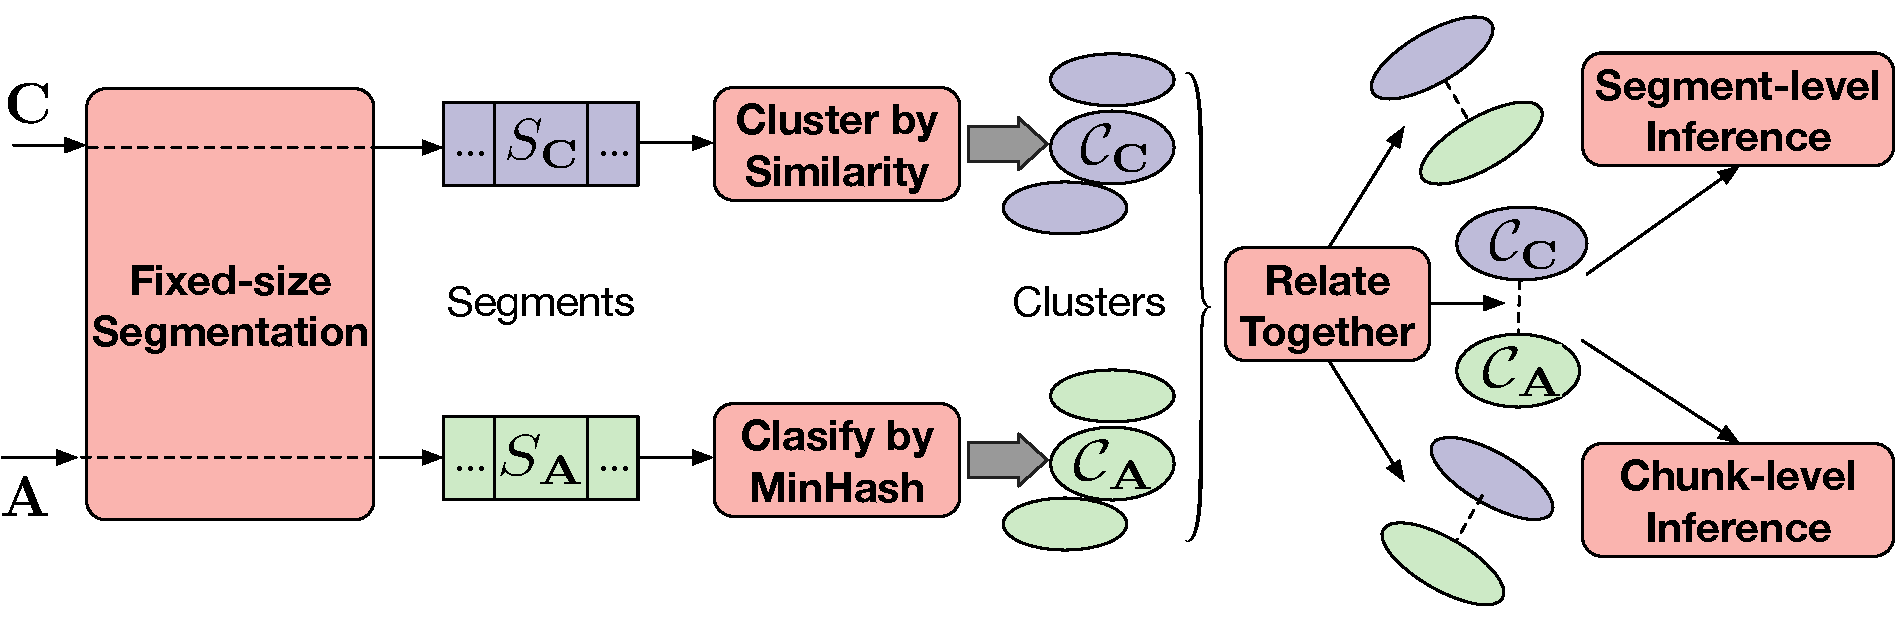
\includegraphics[width=.48\textwidth]{pic/clustering-attack-new.pdf}
    % \caption{Workflow of clustering-based attack: MinHash denotes the minimum chunk hash of plaintext segment, $e(\mathcal{C}_\mathbf{C})$ and $e(\mathcal{C}_\mathbf{A})$ denote the entropies based on the frequency distributions in $\mathcal{C}_\mathbf{C}$ and $\mathcal{C}_\mathbf{A}$, respectively, and  $\#\mathcal{C}_\mathbf{C}$ and $\#\mathcal{C}_\mathbf{A}$ denote the total number of logical ciphertexts and plaintexts in $\mathcal{C}_\mathbf{C}$ and $\mathcal{C}_\mathbf{A}$, respectively.}
    \caption{Workflow of clustering-based attack: MinHash denotes the minimum chunk hash of a plaintext segment.}
	\label{fig:clustering-attack}
\end{figure}

We now present the clustering-based attack (Figure~\ref{fig:clustering-attack}) that builds on similarity to infer original data against encrypted deduplication. 


To exploit similarity, we first introduce {\em segmentation} on a stream of chunks. Specifically, we partition $\mathbf{C}$ into a set of coarse-grained data units, called {\em ciphertext segments}. Each ciphertext segment, denoted by $S_\mathbf{C}$, comprises multiple adjacent ciphertexts in $\mathbf{C}$. In this work, we implement the {\em fixed-size} segmentation scheme to ensure that all ciphertext segments are of the same size (e.g., 4MB by default). 
For compatibility, the same fixed-size segmentation scheme also applies to the auxiliary information $\mathbf{A}$, so as to generate multiple {\em plaintext segments}, each of which is denoted by $S_\mathbf{A}$. 
Note that some variable-size segmentation schemes \cite{lillibridge09, qin17}  identify segment boundaries after the chunks whose contents match a specific pattern and thus address the boundary shift problem faced by the fixed-size segmentation scheme. 
However, we cannot use these variable-size segmentation schemes \cite{lillibridge09, qin17} in the attack. The reason is that the original contents of chunks in ciphertext segments are protected by symmetric encryption, and we cannot ensure that the boundaries for both ciphertext and plaintext segments match the same pattern. This leads to an incompatibility between ciphertext and plaintext segments, and degrades the amount of segment-level data inferred by the clustering-based attack (see the late part of this section).    

% It violates compability, since we cannot   

% It impossible to ensuring the boundaries for  plaintext and ciphertext segments match the same pattern.   

% Even we apply the variable-size segmentation scheme directly  on the contents of ciphertexts, 

% we cannot derive the same pattern for both      



% Note that the order and size of each ciphertext in $\mathbf{C}$ are necessary for operating the fixed-size segmentation, while we do {\em not} need them to reflect those of corresponding plaintext; 


% , so as to be robust against boundary shift of fixed-size segment.  
% we cannot apply
% that match specific content patterns,   
% which address the boundary shift of fixed-size segment, yet requiring to identify segment boundaries that match specific content patterns so as to remain robust against content shifts  
% operate more  requiring the original content patterns of ciphertexts in $\mathbf{C}$. 
 
We propose to infer ciphertext-plaintext pairs through similar segments. Let $S_\mathbf{M}$ be the original plaintext segment of a ciphertext segment $S_\mathbf{C}$ (i.e., each plaintext in $S_\mathbf{M}$ corresponds to some ciphertext in $S_\mathbf{C}$ and vice versa). According to Broder's theorem, if $S_\mathbf{M}$ shares the same minimum chunk hash, say $h$, with some plaintext segment $S_\mathbf{A}$, then $S_\mathbf{M}$  and $S_\mathbf{A}$ tend to have a large fraction of identical plaintexts. This implies that the ciphertexts in $S_\mathbf{C}$ are likely to be mapped from the plaintexts in  $S_\mathbf{A}$. In other words, we first classify all plaintext segments of $\mathbf{A}$ by their minimum chunk hashes, and obtain multiple {\em plaintext clusters}. Each plaintext cluster, denoted by $\mathcal{C}_\mathbf{A} = \{ S_\mathbf{A} \}$, corresponds to a unique minimum chunk hash shared by its included segments. We also 
group the ciphertext segments, whose original plaintext segments have the same minimum chunk hash $h$ (i.e., similar), into an identical {\em ciphertext cluster}, denoted by $\mathcal{C}_\mathbf{C} = \{ S_\mathbf{C} \}$. Then, we infer the original data of $\mathcal{C}_\mathbf{C}$ from some $\mathcal{C}_\mathbf{A}$ that corresponds to  $h$. 

   

% corresponding segment that is mapped to $S_\mathbf{C}$ (i.e., each plaintext in $S_\mathbf{M}$ corresponds to some ciphertext in $S_\mathbf{C}$, and visa versa). 
% Given a ciphertext segment $S_\mathbf{C}$, let 

% if  in other words,  Thus, we propose to launch frequency analysis through similar segments. 
% Specifically,   



% say $\mathcal{C}_\mathbf{C}$.  
% $h$ 
% We denote a plaintext cluster by , which includes multiple  plaintext segments that have the same minimum chunk hash.    
% Each plaintext cluster, denoted by  is a set of  We propose to also collect the ciphertext segments (as a {\em ciphertext cluster} denoted by $\mathcal{C}_\mathbf{C}$) whose original plaintext segments share an identical minimum chunk hash $h$, and then infer their original contents from
% some $\mathcal{C}_\mathbf{A}$ that corresponds to $h$ (i.e., the minimum chunk hash of each plaintext segment in $\mathcal{C}_\mathbf{A}$ equals $h$).    



% and $h$ be the minimum chunk hash computed from $S_\mathbf{M}$.

% Our insight is if $h$ equals the minimum chunk hash of some $S_\mathbf{A}$, then the ciphertexts in $S_\mathbf{C}$  The rationale is the original segment of $S_\mathbf{C}$ has a large fraction of identical plaintexts with $S_\mathbf{A}$ due to Broder's theorem. 



% In other words,   

% This is expected to reduce the disturbances to frequency analysis.  


% $\{S_\mathbf{C}\}$ that have an identical {\em original} minimum element hash $h$,  

% composed of the segments that have the same minimum element hash.  
% However, the original data of each ciphertext segment $S_\mathbf{C}$ is protected by symmetric encryption, and it is impossible to identify the corresponding minimum chunk hash $h$ for grouping ($h$ is derived from the original plaintext segment of $S_\mathbf{C}$). The challenge is how to group similar ciphertext segments {\em without} knowing the minimum chunk hash $h$ of each $S_\mathbf{C}$.    


% the original content of each ciphertext segment $S_\mathbf{C}$ is protected by symmetric encryption; this makes it impossible to identify the corresponding  $h$ for grouping (recall $h$ is derived from the original plaintext segment of $S_\mathbf{C}$). In other words, there exists a challenge of     

We propose a {\em clustering} scheme to group similar ciphertext segments. A na\"{i}ve approach is to classify segments by their minimum chunk hashes, but it does not work on ciphertext segments, whose original contents are protected by symmetric encryption. We address the classification issue based on Broder's theorem.   
% operate classification by the  of each segment , but it .   
Our insight is that if two ciphertext segments have a large fraction of identical ciphertexts, then  they correspond to the same minimum chunk hash with a high probability. The reason is that deterministic encryption preserves the cardinalities of union and intersection of plaintext segments, based on which we can use Broder's theorem to learn the equivalence of their minimum chunk hashes.    
% the fraction of identical plaintexts, based on  Thus, we  apply a clustering algorithm, and aggregate similar ciphertext segments into the same cluster.  

In this work, we define the {\em clustering distance} $d(S_\mathbf{C}, S_\mathbf{C}')$ of any two ciphertext segments $S_\mathbf{C}$ and $S_\mathbf{C}'$ by one minus the fraction of their identical ciphertexts:
\begin{eqnarray}
d(S_\mathbf{C}, S_\mathbf{C}') = 1 - \frac{|S_\mathbf{C} \cap S_\mathbf{C}'|}{|S_\mathbf{C} \cup S_\mathbf{C}'|}. \nonumber
\end{eqnarray}
Note that identical ciphertexts may repeat in $S_\mathbf{C}$ or $S_\mathbf{C}'$, and $|S_\mathbf{C} \cap S_\mathbf{C}'|$ and $|S_\mathbf{C} \cup S_\mathbf{C}'|$ return the number of {\em unique} ciphertexts in their  intersection and union, respectively. Clearly,  the smaller $d(S_\mathbf{C}, S_\mathbf{C}')$ is, the more likely are $S_\mathbf{C}$ and $S_\mathbf{C}'$ to correspond to the same minimum chunk hash. Then, we adopt the {\em agglomerative hierarchical clustering (AHC)} \cite{johnson67} to aggregate similar ciphertext segments based on their distance information.  
Specifically, we start with eash ciphertext segment in its own singleton cluster, and iteratively combine the two closest clusters based on the maximum distance of their ciphertext segments. We configure a parameter $k$, 
% to indicate the upper bound distance in combination, 
and stop the iterated combination when the maximum distance of ciphertext segments in the two cloest
clusters is greater than $k$.


% finally stop combination when       
% Specifically, the clustering scheme is configured by a minimum intercluster distance $d$.   
% We combine nearby segments into clusters based on the distance metric, and stop the combination when 
% the maximum distance between any segment in two clusters is less than $d$.
% the first cluster and any single data point in the second cluster.
% Based on the distance definition, 
% we implement the clustering algorithm via {\em ALGLIB} \cite{alglib}, which is a programming library for extensive data analysis. While ALGLIB supports multiple clustering algorithms, we choose the , because we  only have the distance information of  segments (rather than their coordinates). 
% Specifically, we configure a desired minimum intercluster distance $d$ (e.g., 0.8 by default) via ${\tt clusterizerseparatedbydist()}$, and generate multiple ciphertext clusters via ${\tt clusterizerrunahc()}$.    

For each aggregated ciphertext cluster $\mathcal{C}_\mathbf{C}$, we relate it to some plaintext cluster $\mathcal{C}_\mathbf{A}$ with frequency analysis, while taking frequency distribution into account. This is based on the observation that identical ciphertexts (resp. plaintexts) may  repeat in the same or different ciphertext (resp. plaintext) segments and identical ciphertext (resp. plaintext) segments may also repeat in the same ciphertext (resp. plaintext) cluster. We propose to examine the frequency distribution of the logical ciphertexts or plaintexts in each cluster, and perceive that the frequency distributions for similar clusters (i.e., correspond to the same minimum chunk hash) are also likely to be similar. 
% {\bf Our rationale is changes to backups only apply on limited regions, and do not modify the spatiality of majority chunks.} 

% We proceed the frequency analysis scheme as follows. First, we  sort available ciphertext and plaintext clusters by the total number of logical  ciphertexts and plaintexts they include, respectively. Then, we count the entropy of each cluster based on the frequency distribution of its logical ciphertexts or plaintexts. Like the distribution-based attack (see Section~\ref{sec:distribution-attack-description}), we configure the frequency analysis scheme with the parameters $(u, r, t)$, and infer the ciphertext cluster $\mathcal{C}_\mathbf{C}$ is similar to a plaintext cluster $\mathcal{C}_\mathbf{A}$, if they satisfy the following requirements:    
We proceed the frequency analysis scheme as follows. First, we  sort available ciphertext and plaintext clusters by the total number of logical  ciphertexts and plaintexts they include, respectively. Then, we count an associative array $\mathbf{F}$ that stores the frequency of each unique ciphertext or plaintext in  corresponding cluster. Based on $\mathbf{F}$, we compute the probability that a  ciphertext $C$ exists in a ciphertext cluster $\mathcal{C}_\mathbf{C}$ and further the   
entropy of $\mathcal{C}_\mathbf{C}$:      
% entropy of each ciphertext cluster $\mathcal{C}_\mathbf{C}$:    
\begin{eqnarray*}
    \Pr[C \in \mathcal{C}_\mathbf{C}] = \frac{\mathbf{F}[\mathcal{C}_\mathbf{C}][C]}{\sum_{C' \in \mathcal{C}_\mathbf{C}} \mathbf{F}[\mathcal{C}_\mathbf{C}][C']}, \\
    e(\mathcal{C}_\mathbf{C}) = \sum_{C \in \mathcal{C}_\mathbf{C}} \log_2 \frac{1}{\Pr[C \in \mathcal{C}_\mathbf{C}]},  
    % e(\mathcal{C}_\mathbf{M}) = \sum_{M \in \mathbf{F}[\mathcal{C}_\mathbf{M}]} \log_2 \frac{\mathbf{F}[\mathcal{C}_\mathbf{M}][M]}{a} 
\end{eqnarray*}
where   
$\mathbf{F}[\mathcal{C}_\mathbf{C}][C]$  stores the frequency of $C$ in $\mathcal{C}_\mathbf{C}$. Similarly, we  compute the entropy $e(\mathcal{C}_\mathbf{A})$ for the plaintext cluster $\mathcal{C}_\mathbf{A}$.   
Like the distribution-based attack (see Section~\ref{sec:distribution-attack-description}), we configure the frequency analysis scheme with the parameters $(u, r, t)$, and infer that the ciphertext cluster $\mathcal{C}_\mathbf{C}$ is similar to a plaintext cluster $\mathcal{C}_\mathbf{A}$, if they satisfy the following requirements:
% the entropy of each cluster based on the frequency distribution of its logical ciphertexts or plaintexts. Like the distribution-based attack (see Section~\ref{sec:distribution-attack-description}), we configure the frequency analysis scheme with the parameters $(u, r, t)$, and infer the ciphertext cluster $\mathcal{C}_\mathbf{C}$ is similar to a plaintext cluster $\mathcal{C}_\mathbf{A}$, if they satisfy the following requirements:    
\begin{itemize}[leftmargin=*]
    \item  The rank of $\mathcal{C}_\mathbf{C}$ is not larger than $u$.
    \item  The rank difference of $\mathcal{C}_\mathbf{C}$ and $\mathcal{C}_\mathbf{A}$ is not larger than $r$.  
    \item  The difference of $e(\mathcal{C}_\mathbf{C})$ and $e(\mathcal{C}_\mathbf{A})$ is the smallest and also not larger than $t$.
\end{itemize}

% Thus, the ciphertexts or plaintexts in each cluster may follow a non-uniform frequency distribution, and such frequency distributions are further correlated for the similar clusters  in different backups.  
% We expect  ciphertexts or plaintexts in most of clusters follow a non-uniform frequency distribution, and such frequency distributions are {\em correlated} for  similar clusters (i.e., correspond to the same minimum chunk hash) in different backups. 
% Our rationale is .   
% Thus, we apply a  scheme like the distribution-based frequency analysis (see Section~\ref{sec:distribution-attack-description}), in order to find similar clusters. 

Then, for each pair $(\mathcal{C}_\mathbf{C}, \mathcal{C}_\mathbf{A})$ of similar clusters, we infer ciphertext-plaintext pairs in two levels. 
\begin{itemize}[leftmargin=*]
    \item {\bf Segment-level inference:}
        If $\mathcal{C}_\mathbf{C}$ and $\mathcal{C}_\mathbf{A}$ have the same number of logical chunks (i.e., ciphertexts or plaintexts), as well as an identical entropy, this implies that $\mathcal{C}_\mathbf{C}$ is exactly mapped from $\mathcal{C}_\mathbf{A}$ with a high probability. In this case, we operate attack on the coarse-grained {\em segment} level. Specifically, we first compute the entropies of each ciphertext segment $S_\mathbf{C}$ in $\mathcal{C}_\mathbf{C}$ and each plaintext segment $S_\mathbf{A}$ in $\mathcal{C}_\mathbf{A}$, based on the frequency distributions of their ciphertexts and plaintexts, respectively. 
        % (recall identical chunks may have duplicate copies in the same segment). 
         We infer that $S_\mathbf{C}$ is mapped from  $S_\mathbf{A}$, if the total numbers of logical chunks, as well as the entropies, of $S_\mathbf{C}$ and $S_\mathbf{A}$ are identical. Our evaluation shows that the segment-level inference contributes most of the correctly inferred contents in the
        clustering-based attack (see
        Section~\ref{sec:experiment-clustering}). It is also possible to further recover each plaintext in these inferred segments with additional adversarial knowledge (e.g., ordering). 

        
    \item {\bf Chunk-level inference:}
        If $\mathcal{C}_\mathbf{C}$ and $\mathcal{C}_\mathbf{A}$ have different numbers of logical chunks or entropies, we apply frequency analysis to operate attack on the fine-grained {\em chunk} level. Specifically, we sort all unique ciphertexts and plaintexts by their frequencies in $\mathcal{C}_\mathbf{C}$ and $\mathcal{C}_\mathbf{A}$, respectively, and infer ciphertext-plaintext pairs based on frequency ranks.  
        However, we find the chunk-level inference does not perform well in our experimental dataset. The possible reason is each cluster includes a large number of logical chunks, which degrades the effectiveness of  frequency analysis. Even so, we expect the chunk-level inference can recover more ciphertext-plaintext pairs in practice, especially when the number of logical chunks in some clusters is limited.   
        % there are many tied chunks in the similar classes of the VM dataset
        % Even so, we still expect it can recover even more information in practice, especially when each cluster is of .  
\end{itemize}

% Figure~\ref{fig:clustering-attack} puts all design primitives together, and show the workflow of the clustering-based attack.


\paragraph{Summary:}
To summarize, the clustering-based attack exploits similarity, and launches frequency analysis in similar clusters to infer ciphertext-plaintext pairs. In addition to  $u$, $r$ and $t$, it is configured by the parameter $k$, which specifies the upper bound distance in combining the closest clusters.   

Although possibly affected by the boundary shift of fixed-size segments, we argue that the clustering-based attack is severe against VM disk images. 
Specifically, a flat VM image file is allocated of a fixed size at the time it is created, and such size cannot be changed during its lifetime. All unused regions in a VM image are initially filled with  zero chunks, which can be further re-written for storing additional data in the image. 
% The clustering-based attack does not suffer from boundary shift in this case, since VM images do not need to insert or remove chunks. 
In Section \ref{sec:experiment-clustering}, we examine the effectiveness of the clustering-based attack against VM images.

% One limitation of the clustering-based attack is it suffers from the {\em boundary shift} of segment. Specifically, since we apply fixed-size segmentation, the insertion of one or more chunks will shift the boundaries of all segments that come after the insertion point. This changes the frequency distribution of chunks in some segments, and affects the precision of the identified similar clusters. This also leads to a reduced number of identical segments, and degrades the amount of original contents inferred by the segment-level inference. 
% % Our evaluation shows that the clustering-based attack can only infer about 1\% original content in a long-term backup dataset. 
% We argue that the clustering-based attack is still severe for {\em VM disk images}.    
     

% After allocation, all unused regions in the image are filled by , and   
% which of {\em fixed} sizes during their lifetime.  
% . Specifically, a flat image file is allocated of a {\em fixed} size at the time it is created, and all unused regions of the image file are initially filled with {\em zero chunks}. The image file can store additional data by re-writing zero chunks   
%  Flat images are fixed-size files, with one block for each block in the guest’s disk. Initially, unused blocks are zero-filled; thus, flat disk images tend to have a lot of zero-filled blocks, particularly if they are rela- tively large to allow the guest operating system space into which to store additional data. Sparse images, unlike flat im- ages, only contain virtual disk blocks that have been written at least once. Thus, sparse images can occupy relatively lit- tle space when created, and only grow as the guest operating system uses more and more of its virtual disk. Note, how- ever, that sparse images can
% contain zero-filled blocks, since the guest operating system may write a block containing all zeros; such a block would be stored by the virtual machine in the disk image file. While there is no global standard for virtual machine disk images, specifications for one file format is available from VMware 

% the clustering-based attack has low effectiveness (about 1% inference rate) against the FSL dataset.

% Even so, we argue that the clustering-based attack is severe for some workloads, which store data {\em aligned} with disk block boundaries and do not have the problem of  \cite{jin09}. In \S\ref{sec:experiment-clustering}, we will examine the effectiveness of the clustering-based attack against VM workloads,   



% The main limitation of the clustering-based attack is the {\em boundary shift} of segment.  This changes the chunk distributions of some segments, and  affects the precision of identifying similar classes in Step 2. The boundary shift also decreases the effectiveness of the segment-level attack in Step 3, since it leads to fewer common segments in the auxiliary data and target data. On the other hand, we cannot address the boundary-shift problem by existing approaches (e.g., the content-defined segmentation \cite{lillibridge09}), which depend on the knowledge of the underlying content pattern of ciphertext chunks. 



%% In \S\ref{sec:clustering-experiment}, we justify the barrier of the boundary shift in the clustering-based attack.       
% % between $\mathbf{M}_{\rm a}$ and $\mathbf{M}_{\rm t}$,  
%%We adapt the similarity-based approach to inference attack. Specifically, we apply segmentation, yet on ciphertext chunks, and generate the segments that include adjacent ciphertext chunks under the scrambled order in $\widetilde{\mathcal{L}}_{\rm order}$. 



%If $\mathcal{C}_i$ and $\mathcal{M}_j$ have different numbers of logical chunks or entropies, we apply operate classical frequency analysis to operate attack on {\em chunk level}. This can infer more ciphertext-plaintext chunk pairs, yet degrading inference precision.

%% over $\mathcal{C}_i$ and $\mathcal{M}_j$ . 
%% for each ciphertext segment in $\mathcal{C}_i$, we find the plaintext segment that has the same  
%% Specifically, for each ciphertext segment $S_{\rm t}$ in $\mathcal{C}_i$, we find the plaintext segment $S_{\rm a}$ in $\mathcal{S}_j$ such that   
%% Then, we adopt the idea of distribution-based ranking (\S\ref{sec:distribution-attack-description}) to identify the ciphertext and plaintext classes that are identified by the same MinHash.  
%%In the following, we first propose the {\em similarity-based clustering} approach, which aims to classify ciphertext segments by their underlying MinHash. Then, we elaborate how to relate a class of ciphertext segments with that of plaintext segments. 
%%\paragraph{Similarity-based clustering:}
%%works on ciphertext segments and classify them by their underlying MinHash. Then,   



% \paragraph{Step 3: (Launch attack through similar classes):} For each identified similar classes $(\mathcal{C}_i, \mathcal{M}_j)$, we launch attack for two cases. If $\mathcal{C}_i$ and $\mathcal{M}_j$ have the same number of logical chunks and entropy, our attack operates on {\em segment level}. For each ciphertext segment $S_{\rm t}$ in $\mathcal{C}_i$, we examine each available plaintext segment $S_{\rm a}$ in $\mathcal{S}_j$, and infer $(S_{\rm t}, S_{\rm a})$ as a ciphertext-plaintext segment pair if $S_{\rm a}$ has the same number of logical chunks and entropy (via Equation~\ref{eq:clustering-entropy} but computed for segment) with $S_{\rm t}$. We stop the attack at segment level in this case, because there is not enough information to further extracting chunk content; otherwise it sacrifices inference precision. We argue that the segment-level attack is severe, since each segment represents a continues region of data. The adversary can learn significant information if it successfully extracts the underlying data of some segment. 

%% Through experimental analysis, the segment-level attack contributes the most component of correct inferences.     
%% has the same number of logical chunks and entropy as $S_{\rm t}$. We infer that $S_{\rm a}$ is the original segment of $S_{\rm t}$. 

%If $\mathcal{C}_i$ and $\mathcal{M}_j$ have different numbers of logical chunks or entropies, we apply operate classical frequency analysis to operate attack on {\em chunk level}. This can infer more ciphertext-plaintext chunk pairs, yet degrading inference precision.

%% over $\mathcal{C}_i$ and $\mathcal{M}_j$ . 
%% for each ciphertext segment in $\mathcal{C}_i$, we find the plaintext segment that has the same  
%% Specifically, for each ciphertext segment $S_{\rm t}$ in $\mathcal{C}_i$, we find the plaintext segment $S_{\rm a}$ in $\mathcal{S}_j$ such that   
%% Then, we adopt the idea of distribution-based ranking (\S\ref{sec:distribution-attack-description}) to identify the ciphertext and plaintext classes that are identified by the same MinHash.  
%%In the following, we first propose the {\em similarity-based clustering} approach, which aims to classify ciphertext segments by their underlying MinHash. Then, we elaborate how to relate a class of ciphertext segments with that of plaintext segments. 
%%\paragraph{Similarity-based clustering:}
%%works on ciphertext segments and classify them by their underlying MinHash. Then,   



% Based on the configuration parameters of $u$, $r$ and $t$ (see \S\ref{sec:distribution-attack-description}), we pick the ciphertext class $\mathcal{C}_i$ that has the $i$-th most number of logical chunks ($1 \leq i \leq u$), and examine each plaintext class $\mathcal{M}_j$ that ranks from $i-r$ to $i+r$. We identify that $\mathcal{C}_i$ and $\mathcal{M}_j$ have the same MinHash, if the difference of their entropies is (i) minimum across all $i-r \leq j \leq i+r$ and (ii) smaller than $t$.   

   

% while the rest data preserve the same characteristics.   
% Due to backup redundancies, .   . 
% Our rationale is that the chunk distributions in similar classes are likely to be correlated due to deterministic encryption.

%We build on the idea of the distribution-based ranking (see \S\ref{sec:distribution-attack-description}) to identify the ciphertext and plaintext classes that correspond to the same MinHash. Specifically, for each ciphertext class with an underlying MinHash of $h$, our aim is to find the plaintext class identified by the same MinHash of $h$. Note that we cannot measure relative frequency distributions for ranking, since we do not have enough knowledge about neighboring chunks. Instead, we count the entropy of a class by the {\em occurrences of different chunks} in the class. Specifically, for a plaintext class $\mathcal{M}$, we compute its entropy:  \begin{eqnarray}
%        e_{\mathcal{M}} = \sum_{M \in \mathcal{M}} {\sf log}_2 \frac{{\sf cnt}_\mathcal{M}(M)}{|\mathcal{M}|},
%        \label{eq:clustering-entropy}
%\end{eqnarray}
%where $|\mathcal{M}|$ is the total number of logical chunks in $\mathcal{M}$ and ${\sf cnt}_\mathcal{M}(M)$ returns the number of copies of the chunk $M$ in $\mathcal{M}$. We derive similar entropy $e_\mathcal{C}$ for a ciphertext class $\mathcal{C}$, and consider $\mathcal{M}$ and $\mathcal{C}$ are {\em similar classes} (i.e., having the same MinHash), if the difference of their entropies is minimum. Our rationale is that the chunk distributions in similar classes are likely to be correlated due to deterministic encryption.  

%In more details, we first sort the available ciphertext and plaintext classes separately by the number of logical chunks they include. Based on the configuration parameters of $u$, $r$ and $t$ (see \S\ref{sec:distribution-attack-description}), we pick the ciphertext class $\mathcal{C}_i$ that has the $i$-th most number of logical chunks ($1 \leq i \leq u$), and examine each plaintext class $\mathcal{M}_j$ that ranks from $i-r$ to $i+r$. We identify that $\mathcal{C}_i$ and $\mathcal{M}_j$ have the same MinHash, if the difference of their entropies is (i) minimum across all $i-r \leq j \leq i+r$ and (ii) smaller than $t$.   

%% However, it is hard to classify ciphertext segments, since there still exists a challenge on identifying the underlying MinHash of ciphertext segments. Recall that  
%% By our assumption (\S\ref{sec:clustering-attack}), all ciphertext segments must have the same size. Thus, to be compatible, we also partition the original stream of plaintext chunks $\mathbf{M}_{\rm a}$ into fixed-size {\em plaintext segments}, each of which comprises a sequence of plaintext chunks.

%% We adapt the similarity-based approach to inference attack. Specifically, to capture the notion of similarity,  
%% for inferring ciphertext-plaintext chunk pairs through similar segments. Specifically, we   



% We proceed our similarity-based clustering scheme as follows. It defines the {\em clustering distance} of The smaller the distance ${\sf Dist}(S_{\rm t}, S_{\rm t}')$ is, the more likely are $S_{\rm t}$ and $S_{\rm t}'$ to have the same underlying MinHash. Then, it uses the agglomerative hierarchical clustering algorithm (via the function  in ) for clustering, and generates the ciphertext classes based on a desired minimum intercluster distance of $d$ (via the function  in ALGLIB \cite{alglib}). By default, we configure $d$ by 0.8. 



% we can apply Broder's theorem  on ciphertexts due to the deterministic nature of encryption.  
% This is because encryption preserves the deduplication capability of elements.
% . Thus, we can compute the overlaps between any two ciphertext segments, and cluster them into several {\em ciphertext classes}, such that each cluster includes the ciphertext segments that possibly have the same underlying MinHash.    

 


%We propose the {\em similarity-based clustering} approach, which aims to classify the ciphertext segments by their underlying MinHash while not compromising confidentiality. The key insight is that if two ciphertext segments have a large fraction of common (ciphertext) chunks, then they are likely to have the same underlying MinHash (due to Equation (\ref{eq:broder})). Thus, we can compute the overlaps between any two ciphertext segments, and cluster them into several {\em ciphertext classes}, such that each cluster includes the ciphertext segments that possibly have the same underlying MinHash.    




% identify  This raises a challenge on how to group   
% the minimum element hash $h$  
% it is impossible to the original plaintext and identify the minimum element hash corresponding to a ciphertext segment.  
% recover its original plaintext segment and extract the minimum element hash.    
% the original plaintexts of the ciphertext segment, and further learn the      
% The challenge is  Since each ciphertext segment is mapped by symmetric encryption, it is impossible to learn their original content and identify the minimum element hash from corresponding plaintexts.
% Since each ciphertext in $S_\mathbf{C}$ is mapped by symmetric encryption, it is impossible to learn their original plaintexts or identify the minimum element hash (based on these plaintexts). In other words, the main challenge  
% which chunk leads to the minimum element hash, and further the exact hash value. In other words, there exists a challenge on collecting similar $\{ S_\mathbf{C} \}$ (i.e., they share the same original minimum element hash) and map them to $\mathcal{C}_\mathbf{A}$. 


%Thus, instead of inferring ciphertext-plaintext pairs (from $\mathbf{C}$ and $\mathbf{A}$) directly,     


%One challenge behind the clustering-based attack is how to identify the original minimum element hash $h$ of each $S_\mathbf{C}$. Since       


%The clustering-based attack proceeds as follows. First, we  


%We classify plaintext segments into a set of {\em plaintext classes} by their MinHash. On the other hand, we cannot perform similar classification over ciphertext segments, since their underlying contents are protected by symmetric encryption (see \S\ref{sec:threat}). 

%% , each of which includes the plaintext segments that have the same MinHash. 
%% it is impossible to access or compare the underlying contents of ciphertext chunks for classification, since their original contents are protected by symmetric encryption   


%% split the original space () of frequency analysis into multiple subspaces, and
%% eliminates     
%% identify the minimum element hash of each $S_\mathbf{C}$, and then apply frequency analysis with some $S_\mathbf{A}$ that shares the same minimum element hash. This      
%% This inspires us to    
% % $S_\mathbf{M}$ has a large fraction of overlaps with the original plaintexts of $S_{\rm t}$    
%% Our insight is  if the {\em underlying MinHash} (that is computed from the plaintext of each ciphertext chunk element) of a ciphertext segment $S_{\rm t}$ is identified the same as that of some plaintext segment $S_{\rm a}$, then the chunks in $S_{\rm a}$ are likely to be the original plaintexts of the ciphertexts in $S_{\rm t}$. The rationale is that $S_{\rm a}$ has a large fraction of overlaps with the original plaintexts of $S_{\rm t}$  (due to Equation~(\ref{eq:broder})). In other words, we collect all ciphertext segments that have a common underlying MinHash (see Step 1), say $h$, and infer their original chunks from the plaintext segments that have the same MinHash of $h$ (see Step 2 and Step 3). By repeating the inference for each available MinHash, we can avoid some of ties incurred by classical frequency analysis, since the tied chunks may have different frequencies for the same MinHash.    
%% Similarly, we apply fixed-size segmentation to generate each segment $S_\mathbf{A}$ that consists of plaintexts of $\mathbf{A}$.
%% knowledge of the underlying content pattern of ciphertext chunks. 
%% that we need the order of each ciphertext in $\mathbf{C}$ for segmentation, while not requiring such order reflects that of corresponding plaintext. 
%% We use  and  that is generated from $\mathbf{C}$ and that is mapped from, respectively.
%% generated from $\mathbf{C}$ and its corresponding plaintext, respectively.
%% denote a segment from $\mathbf{C}$ by  
%% Note that we need the ordering of $\mathbf{C}$ to ensure each segment includes the continue content, while not requiring such ordering reflects that of corresponding plaintext.  
%% {\em fixed-size} data units,   
%%In this work, we implement fixed-size segmentation scheme to generate ciphertext segments. More sophisticated segmentation schemes (e.g., variable-size segmentation \cite{lillibridge09, qin17}) can be applied to address content shifting, yet they depend on the knowledge of the underlying content pattern of ciphertext chunks. For clustering, we define the distance of two ciphertext segments $S_{\rm tar}$ and $S_{\rm tar}'$ by one minus their Jaccard similarity coefficient:
%%
%% Given $\mathbf{C}$, we partition   
%% The clustering-based attack builds on {\em similarity-based approach} \cite{li17,qin17,xia11,bhagwat09}. Specifically, the similarity-based approach groups multiple adjacent chunks into a coarse-grained unit called {\em segment}, and considers that two segments are {\em similar} if they have the same minimum hash value (i.e., {\em MinHash}) over their chunk elements. By Broder's theorem \cite{broder97}, the probability that two segments $S$ and $S'$ are similar is the same as their Jaccard similarity coefficient: 
%% \subsection{Attack Description}
%% {\color{blue}
%% {\bf --- not good enough ---}
%% To capture similarity in inference attack, we partition the auxiliary stream $\mathbf{M}_{\rm a}$ of plaintext chunks into {\em plaintext segments}, which comprises sequences of plaintext chunks. Correspondingly, we construct {\em ciphertext segments}, each of which is composed of the ciphertext chunks whose original plaintexts are in the same plaintext segment. For compatibility, we ensure that both  plaintext and ciphertext segments have the same size.   
%% {\bf --- not good enough ---}
%% }
%% (recall that we can access the time windows of original chunks from $\widetilde{\mathcal{L}}_{\rm order}$). 
%% We propose to launch inference attack through similar segments. 


%\begin{figure}
%	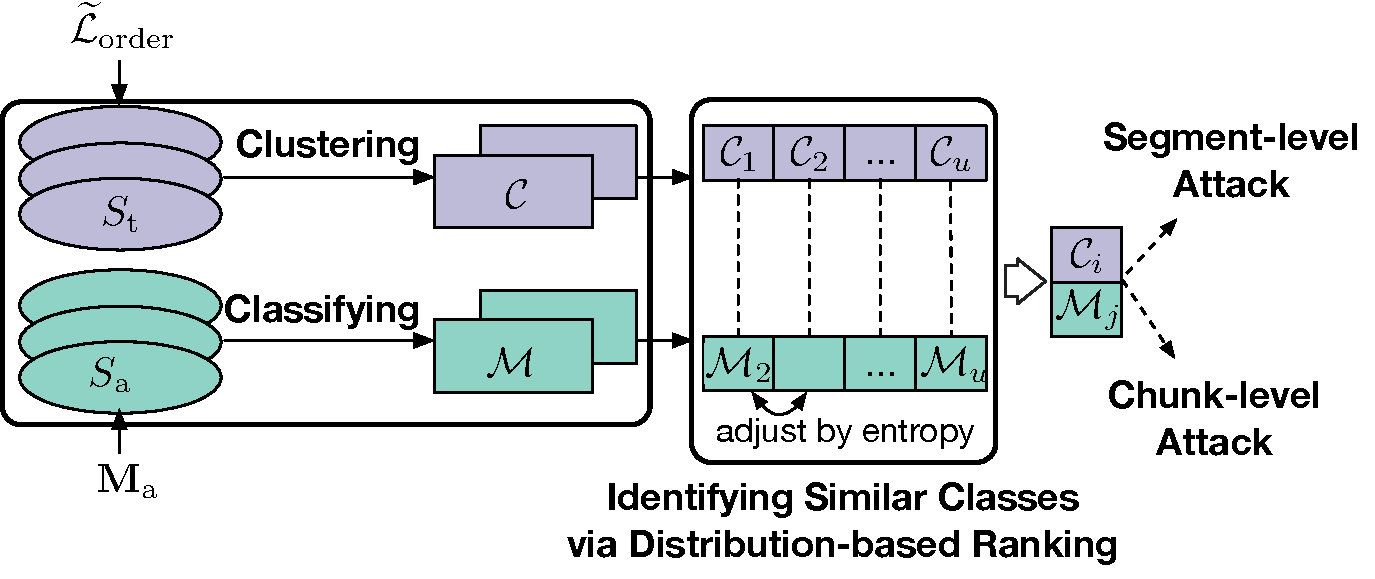
\includegraphics[width=.48\textwidth]{pic/clustering-attack.pdf}
%	\caption{Overview of the clustering-based attack.}
%	\label{fig:clustering-attack}
%\end{figure}

%Figure~\ref{fig:clustering-attack} highlights the main steps of the clustering-based attack. We elaborate the details as follows. 


%\paragraph{Step 2: (Identify similar classes):}
%We build on the idea of the distribution-based ranking (see \S\ref{sec:distribution-attack-description}) to identify the ciphertext and plaintext classes that correspond to the same MinHash. Specifically, for each ciphertext class with an underlying MinHash of $h$, our aim is to find the plaintext class identified by the same MinHash of $h$. Note that we cannot measure relative frequency distributions for ranking, since we do not have enough knowledge about neighboring chunks. Instead, we count the entropy of a class by the {\em occurrences of different chunks} in the class. Specifically, for a plaintext class $\mathcal{M}$, we compute its entropy:  \begin{eqnarray}
%        e_{\mathcal{M}} = \sum_{M \in \mathcal{M}} {\sf log}_2 \frac{{\sf cnt}_\mathcal{M}(M)}{|\mathcal{M}|},
%        \label{eq:clustering-entropy}
%\end{eqnarray}
%where $|\mathcal{M}|$ is the total number of logical chunks in $\mathcal{M}$ and ${\sf cnt}_\mathcal{M}(M)$ returns the number of copies of the chunk $M$ in $\mathcal{M}$. We derive similar entropy $e_\mathcal{C}$ for a ciphertext class $\mathcal{C}$, and consider $\mathcal{M}$ and $\mathcal{C}$ are {\em similar classes} (i.e., having the same MinHash), if the difference of their entropies is minimum. Our rationale is that the chunk distributions in similar classes are likely to be correlated due to deterministic encryption.  


%In more details, we first sort the available ciphertext and plaintext classes separately by the number of logical chunks they include. Based on the configuration parameters of $u$, $r$ and $t$ (see \S\ref{sec:distribution-attack-description}), we pick the ciphertext class $\mathcal{C}_i$ that has the $i$-th most number of logical chunks ($1 \leq i \leq u$), and examine each plaintext class $\mathcal{M}_j$ that ranks from $i-r$ to $i+r$. We identify that $\mathcal{C}_i$ and $\mathcal{M}_j$ have the same MinHash, if the difference of their entropies is (i) minimum across all $i-r \leq j \leq i+r$ and (ii) smaller than $t$.   

%% However, it is hard to classify ciphertext segments, since there still exists a challenge on identifying the underlying MinHash of ciphertext segments. Recall that  
%% By our assumption (\S\ref{sec:clustering-attack}), all ciphertext segments must have the same size. Thus, to be compatible, we also partition the original stream of plaintext chunks $\mathbf{M}_{\rm a}$ into fixed-size {\em plaintext segments}, each of which comprises a sequence of plaintext chunks.

%% We adapt the similarity-based approach to inference attack. Specifically, to capture the notion of similarity,  
%% for inferring ciphertext-plaintext chunk pairs through similar segments. Specifically, we   


%\paragraph{Step 3: (Launch attack through similar classes):} For each identified similar classes $(\mathcal{C}_i, \mathcal{M}_j)$, we launch attack for two cases. If $\mathcal{C}_i$ and $\mathcal{M}_j$ have the same number of logical chunks and entropy, our attack operates on {\em segment level}. For each ciphertext segment $S_{\rm t}$ in $\mathcal{C}_i$, we examine each available plaintext segment $S_{\rm a}$ in $\mathcal{S}_j$, and infer $(S_{\rm t}, S_{\rm a})$ as a ciphertext-plaintext segment pair if $S_{\rm a}$ has the same number of logical chunks and entropy (via Equation~\ref{eq:clustering-entropy} but computed for segment) with $S_{\rm t}$. We stop the attack at segment level in this case, because there is not enough information to further extracting chunk content; otherwise it sacrifices inference precision. We argue that the segment-level attack is severe, since each segment represents a continues region of data. The adversary can learn significant information if it successfully extracts the underlying data of some segment. 


%% Through experimental analysis, the segment-level attack contributes the most component of correct inferences.     
%% has the same number of logical chunks and entropy as $S_{\rm t}$. We infer that $S_{\rm a}$ is the original segment of $S_{\rm t}$. 

%If $\mathcal{C}_i$ and $\mathcal{M}_j$ have different numbers of logical chunks or entropies, we apply operate classical frequency analysis to operate attack on {\em chunk level}. This can infer more ciphertext-plaintext chunk pairs, yet degrading inference precision.

%% over $\mathcal{C}_i$ and $\mathcal{M}_j$ . 
%% for each ciphertext segment in $\mathcal{C}_i$, we find the plaintext segment that has the same  
%% Specifically, for each ciphertext segment $S_{\rm t}$ in $\mathcal{C}_i$, we find the plaintext segment $S_{\rm a}$ in $\mathcal{S}_j$ such that   
%% Then, we adopt the idea of distribution-based ranking (\S\ref{sec:distribution-attack-description}) to identify the ciphertext and plaintext classes that are identified by the same MinHash.  
%%In the following, we first propose the {\em similarity-based clustering} approach, which aims to classify ciphertext segments by their underlying MinHash. Then, we elaborate how to relate a class of ciphertext segments with that of plaintext segments. 
%%\paragraph{Similarity-based clustering:}
%%works on ciphertext segments and classify them by their underlying MinHash. Then,   

%\subsection{Discussion}
%\label{sec:clustering-attack-discussion}

%The main limitation of the clustering-based attack is the {\em boundary shift} of segment. The insertion of one or more chunks will shift the boundaries of all segments that come after the insertion point. This changes the chunk distributions of some segments, and  affects the precision of identifying similar classes in Step 2. The boundary shift also decreases the effectiveness of the segment-level attack in Step 3, since it leads to fewer common segments in the auxiliary data and target data. On the other hand, we cannot address the boundary-shift problem by existing approaches (e.g., the content-defined segmentation \cite{lillibridge09}), which depend on the knowledge of the underlying content pattern of ciphertext chunks. 


%Even so, we argue that the clustering-based attack is severe for the virtual machine (VM) images, which store data {\em aligned} with disk block boundaries  \cite{jin09}. In \S\ref{sec:experiment-clustering}, we will examine the effectiveness of the clustering-based attack against VM workloads. 



%% In \S\ref{sec:clustering-experiment}, we justify the barrier of the boundary shift in the clustering-based attack.       
% % between $\mathbf{M}_{\rm a}$ and $\mathbf{M}_{\rm t}$,  
%%We adapt the similarity-based approach to inference attack. Specifically, we apply segmentation, yet on ciphertext chunks, and generate the segments that include adjacent ciphertext chunks under the scrambled order in $\widetilde{\mathcal{L}}_{\rm order}$. 


%%In this work, we implement fixed-size segmentation scheme to generate ciphertext segments. More sophisticated segmentation schemes (e.g., variable-size segmentation \cite{lillibridge09, qin17}) can be applied to address content shifting, yet they depend on the knowledge of the underlying content pattern of ciphertext chunks. For clustering, we define the distance of two ciphertext segments $S_{\rm tar}$ and $S_{\rm tar}'$ by one minus their Jaccard similarity coefficient:
%%$${\sf Sim}(S_{\rm tar}, S_{\rm tar}') = 1 - \frac{|S_{\rm tar} \cap S_{\rm tar}'|}{|S_{\rm tar} \cup S_{\rm tar}'|}.$$
%%The smaller ${\sf Sim}(S_{\rm tar}, S_{\rm tar}')$ is, the more likely that they have the same underlying MinHash. Then, we use agglomerative hierarchical clustering algorithm (via the function {\tt clusterizerrunahc} in ALGLIB \cite{alglib}) to generate the slices. 

%%% For any two ciphertext segments $S_{\rm tar}$ and $S_{\rm tar}'$, we define their similarity distance by one minus their Jaccard similarity coefficient:
%%% $${\sf Sim}(S_{\rm tar}, S_{\rm tar}') = 1 - \frac{|S_{\rm tar} \cap S_{\rm tar}'|}{|S_{\rm tar} \cup S_{\rm tar}'|}.$$

%%In addition, we partition $\mathbf{M}_{\rm aux}$ to form plaintext segments, each of which is a region of logically adjacent chunks in $\mathbf{M}_{\rm aux}$. For compatibility, we require that the plaintext segment has the same (fixed) size with ciphertext segment. Then, we classify plaintext segments by their MinHash (note that we have full access to the MinHash of each plaintext segment), and obtain several plaintext slices. 

%%To launch attack, we apply frequency analysis to the ciphertext and plaintext slices that are identified by the same MinHash. This is for two reasons. First, tied chunks may have different frequencies in some slices, and these ties can be break. Second, the original chunks are likely to be in the 

%%each of which includes the segments that have the same MinHash (note that we have fully access to the MinHash of each plaintext segment).   



%%Like prior works \cite{li17,qin17,xia11,bhagwat09}, we   




%%Specifically, we  We also generate ciphertext segments, which include adjacent ciphertext chunks yet under the scrambled order in $\widetilde{\mathcal{L}}_{\rm order}$. 



%%The clustering-based attack uses {\em ``divide-and-conquer''} strategy to improve the inference accuracy of tied chunks. At a high level, it partitions $\mathbf{M}_{\rm aux}$ into {\em plaintext slices}, and each slice includes a number of plaintext chunks. It generates similar {\em ciphertext slices} from $\widetilde{\mathcal{L}}_{\rm order}$, and pairs each ciphertext slice with some plaintext slice of $\mathbf{M}_{\rm aux}$. It finally applies frequency analysis to infer original chunks from each slice pair. The rationale is that tied chunks may have different frequencies in some slices.

%%% To generate slices, we build on the {\em similarity-based approach} \cite{li17,qin17,xia11,bhagwat09}. Specifically, it defines a coarse-grained unit called {\em segment}, which comprises multiple adjacent chunks. Two segments are said {\em similar}, if they have the same minimum hash (i.e., MinHash) over their chunk elements. By Broder's theorem \cite{broder97}, the probability that two segments $S_i, S_j$ are similar is the same as their Jaccard similarity coefficient: 
%%% $${\sf Pr}[{\sf MinHash}(S_i) = {\sf MinHash}(S_j)] = \frac{|S_i \cap S_j|}{|S_i \cup S_j|},$$
%%% where ${\sf MinHash}(S)$ is the minimum hash of chunk element in $S$. Thus, prior works \cite{li17,qin17,xia11,bhagwat09} can apply the similarity-based approach to improve the effectiveness of near-exact deduplication. 


%%To form a plaintext slice, we collect all     


%%===


%%Specifically, we add the segments that have the same MinHash into an identical slice, and pair a ciphertext slice with a plaintext slice if they have the same chunk. Thus,  

%%each slice includes the segments that have the same MinHash. Since 

%%the original chunk of ciphertext chunk is likely to be in  


%%Our insight is that if two ciphertext segments have a large fraction of common chunks, they are likely to have the same underlying MinHash.


%%By Broder's theorem, similar segments are likely to have a large fraction of common chunks.  


%%Our insight is to generate slices  



%%A plaintext segment is a region of logically adjacent chunks in $\mathbf{M}_{\rm aux}$, while a ciphertext segment includes several adjacent ciphertext chunks defined in the scrambled order in $\widetilde{\mathcal{L}}_{\rm order}$. We measure the {\em similarity} of two segments (e.g., $S_i$ and $S_j$) by their Jaccard similarity coefficient (e.g., $|S_i \cap S_j|/|S_i \cup S_j|$).     

%%Our insight is to generate the slices that include all segments identified by the same MinHash.  



%%We propose a new inference attack, the {\em clustering-based attack}, which uses {\em ``divide-and-conquer''} strategy to improve the severity of frequency analysis.   
   

%%The clustering-based attack builds on  




%%The key technique underlying the attack is {\em similarity-based approach} to generate slices.  

%%To generate slices, the clustering-based attack uses a {\em similarity-based approach}, which builds on a coarse-grained unit, called {\em segment}, of chunks. A plaintext segment is a region of logically adjacent chunks in $\mathbf{M}_{\rm aux}$. We also extract ciphertext segments, which include adjacent ciphertext chunks defined in the scrambled order in $\widetilde{\mathcal{L}}_{\rm order}$.   





%%It can  based    


%%We generate a plaintext segment as a region of  On the other hand, we form ciphertext segments directly based on the scrambled order of each ciphertext chunk. 




%%Specifically, 


%%   which can infer original chunk content with coarse-grained order information. 
   


%%In the following, we present the attack details step by step.

%%% We propose the {\em clustering-based attack}. At a high level, it partitions $\mathbf{M}_{\rm aux}$ into {\em plaintext slices}, which include a number of plaintext chunks. It generates similar {\em ciphertext slices} from $\widetilde{\mathcal{L}}_{\rm order}$, and pairs each ciphertext slice with some plaintext slice of $\mathbf{M}_{\rm aux}$. It finally applies frequency analysis to infer original chunks from each ciphertext-plaintext slice pair. In the following, we present the attack step by step.

%%\paragraph{Step 1: Group chunks into segments.}
%%The clustering-based attack defines a coarse-grained unit, called {\em segment}, of chunks. We generate a plaintext segment as a region of logically adjacent chunks in $\mathbf{M}_{\rm aux}$. On the other hand, we form ciphertext segments directly based on the scrambled order of each ciphertext chunk. 

%%By segmentation, we expect we can limit order scrambling within each segment.


%%Note that since we cannot identify the underlying content of ciphertext chunks, our segmentation scheme is with a fixed size rather than content based.    



%%it can only form ciphertext segment based on the scrambled orders of ciphertext chunks. Even so, we expect the order scrambling can be located within each segment.    

 
%%By segmentation, we expect the order 


%%For $\mathbf{M}_{\rm aux}$, a (plaintext) segment includes a fixed-size region of logically adjacent chunks. On the other hand, we cannot identify the accurate order of each ciphertext chunk. Thus, we elaborate segment as based on the scrambled orders in $\widetilde{\mathcal{L}}_{\rm order}$. 


%%\paragraph{Step 2: Classify plaintext segments by MinHash.}

%%\paragraph{Step 3: Cluster ciphertext segments by similarity.}





%%% The rationale is that tied chunks may have different frequencies in some slices.  


%%The clustering-based attack builds on a {\em similarity-based approach} to generate slices of chunks. First, it groups chunks into a coarse-grained unit, called {\em segment}. 

%%After segmentation, we expect the order scrambling only appears within each segment.

%%\paragraph{Step 3: Slice pairing.}

%%\paragraph{Step 4: Chunk inference.}








%%We start with a na\"{i}ve slicing approach. Specifically, we partition $\mathbf{M}_{\rm aux}$ into fixed-size regions of   

%%To realize slicing, we propose a  
%%generates plaintext and ciphertext slices from $\mathbf{M}_{\rm aux}$ and $\widetilde{\mathcal{L}}_{\rm order}$, respectively. Each slice includes a number of plaintext or ciphertext chunks.    


%%To generate slices, the attack builds on the similarity characteristics of workloads.  

%%The attack apply to pair ciphertext-plaintext slices,


%%First, the adversary 



%%We start with a na\"ive frequency analysis. 


%%builds on similarity. 

%%\paragraph{Similarity-based clustering:}

%%\paragraph{Distribution-based pairing:}

%%At a high level, the clustering-based attack partitions $\mathbf{M}_{\rm aux}$ into {\em plaintext slices}, and each slice includes a number of plaintext chunks. It also generates ciphertext slices from $\widetilde{\mathcal{L}}_{\rm order}$, and pairs each ciphertext slice with some plaintext slice of $\mathbf{M}_{\rm aux}$. Then, it applies frequency analysis on all paired ciphertext-plaintext slices to infer chunks.   


%%The similarity-based clustering builds on Broder's theorem, which states that the probability that the two sets $S_1$ and $S_2$ have the same minimum hash element is the same as their Jaccard similarity coefficient. 

%%\subsection{Attack Description}

%%Our idea is to group all chunks






%%We first overview how the clustering-based attack works.  First, the adversary partitions $\mathbf{M}_{\rm aux}$ into {\em plaintext slices}, and each slice includes a number of plaintext chunks. It also generates ciphertext slices from $\widetilde{\mathcal{L}}_{\rm order}$. Then, the adversary pairs each ciphertext slice with some plaintext slice, and applies frequency analysis on all paired slices to infer chunks. This mitigates the chunk tiles in some extent, since the globally tied chunks may not have the same frequency in all paired slices.  


%%at high level. Generally, the clustering-based attack builds on the  It partitions 

%%The clustering-based attack builds on the  strategy. Specifically, it cuts $\mathbf{M}_{\rm aux}$ into several {\em plaintext slices}, and each slice includes a number of plaintext chunks.     

%%A naive slicing solution is to 

%%Based on the auxiliary information, it 


%%Instead of attacking with $\mathbf{M}_{\rm aux}$ and $\widetilde{\mathcal{L}}_{\rm order}$ in their entirety, it divides the adversarial knowledge into plaintext and ciphertext slices, and uses frequency analysis to identify the ciphertext-plaintext chunks in each slice.    


%%Specifically, it first generates plaintext slices $\mathbf{M}_{\rm aux}$. Each slice includes a number of continuous chunks.   

%%\paragraph{Attack details:}

%%\subsection{Discussion}




%%%in which the known chunk orders are {\em permuted} from the original order of corresponding chunks. 



%%%We first re-define our model to adapt the setting of the two-stage attack.   
   
   
%%%   which requires {\em minimum} knowledge about order information. Specifically, in the two-stage attack, the  instead, it just need to access  


%%%can work with  

%%%only needs {\em minimum} knowledge about order information. Specifically, it can build on  


%%%We suppose that the target victim file $\mathbf{M}_{\rm tar}$ includes $n$ chunks (including duplicates), and $\pi$ is a permutation by randomizing the logical orders of every $k$ chunks. 

%%%over their order set $\{1,\ldots,n\}$.







%%%%We define $\widetilde{\mathcal{L}}_{\rm order} = \{(C, \pi({\sf ord}(M))): (M, *) \in \mathbf{M}_{\rm tar} \wedge C = \mathcal{E}_K(M)\}$.

%%%{\bf TO DO}
%%%% suppose the target victim file includes $n$ logical chunks, and $\pi$ is a permutation on the set $\{1,\ldots,n\}$. }

%%%\paragraph{Attack Overview:}

%%%\subsection{Attack Overview}

%%%The two-stage attack follows the {\em divide and conquer} principle. Figure \ref{fig:overview} outlines the overview of the two-stage attack.  



%%\subsection{Similarity-based Clustering}

%%\subsection{Attack Description}

%%\subsection{Attack Example}

\chapter{Experiments}
\label{sec:experiment}

In this section, we present the trace-driven evaluation results to demonstrate
the severity of our proposed frequency analysis attacks against encrypted
deduplication.

\section{Methodology}
\label{sec:dataset}

\begin{table}[!t]
    \caption{Characteristics of experimental datasets.}
\small
\label{tab:dataset}
\renewcommand{\arraystretch}{1.2}
\vspace{-3pt}
\centering
\begin{tabular}{|c|c|c|c|}
\hline
 \multirow{2}{*}{\bf Dataset} & \multirow{2}{*}{\bf Category} & \multicolumn{2}{c|}{\bf Characteristics in Each Snapshot} \\
\cline{3-4}
    & &  \#Logical (Million) & \#Unique (Million) \\
\hline
    \multirow{6}{*}{FSL} & User004  & 1.0-1.3 & 0.7-0.9\\
 \cline{2-4}
              & User007 &  3.5-5.2 & 2.3-3.6 \\
 \cline{2-4}
              & User012 &  25.0-26.4 & 8.9-9.7 \\
\cline{2-4}
              & User013 &  1.8-5.7 & 1.2-4.2 \\
\cline{2-4}
              & User015 &  13.4-20.5 & 9.0-11.0 \\
\cline{2-4}
              & User028 &  6.0-10.3 & 3.5-6.8 \\
\hline
\hline
    \multirow{4}{*}{MS} & Win7  & 61.6-61.8 & 61.1-61.3\\
\cline{2-4}
              & Serv-03 & 10.6-10.7 & 8.4-8.5\\
\cline{2-4}
              & Serv-08 & $\sim$6.5 & $\sim$3.8 \\
\cline{2-4}
              & Vista-B &  $\sim$7.6 & $\sim$2.0\\
\cline{2-4}
              & Vista-U &  $\sim$21.0 & $\sim$10.4 \\
\hline
\hline

    \multirow{6}{*}{VM} & User1  &  \multirow{6}{*}{2.6} & $\sim$0.9 \\
\cline{2-2}
\cline{4-4}
              & User2 &  & 1.1-1.3 \\
\cline{2-2}
\cline{4-4}
              & User3 &  & 0.9-1.1 \\
\cline{2-2}
\cline{4-4}
              & User4 &  & $\sim$0.9 \\
\cline{2-2}
\cline{4-4}
              & User5 &  & 0.9-1.0 \\
\cline{2-2}
\cline{4-4}
              & User6 &  & 0.9-1.1 \\
\hline
\end{tabular}
\medskip

\raggedright
    The notations \#Logical and \#Unique denote the total number of logical and unique chunks in each experimental snapshot, respectively. 
    % All VM images have a fixed size of 10GB and hence the same number of logical chunks.
\end{table}



%\begin{table}[!t]
%\small
%\caption{Experimental datasets.}
%\label{tab:dataset}
%\renewcommand{\arraystretch}{1.2}
%\vspace{-3pt}
%\centering
%\begin{tabular}{|c|c|c|}
%\hline
%{\bf Dataset} & {\bf Category} & {\bf Approximate Logical Size} \\
%\hline
%\hline
%%\multirow{2}{*}{FSL} & Physical  & 431.9GB  & 659.3GB & 584.3GB \\
%	\multirow{6}{*}{FSL} & User004  & 10GB/backup $\times$ 14 backups \\
%\cline{2-3}
%			  & User007 & 39GB/backup $\times$ 14 backups \\
%\cline{2-3}
%			  & User012 & 244GB/backup $\times$ 14 backups \\
%\cline{2-3}
%			  & User013 & 22GB/backup $\times$ 14 backups\\
%\cline{2-3}
%			  & User015 & 158GB/backup $\times$ 14 backups\\
%\cline{2-3}
%			  & User028 & 77GB/backup $\times$ 14 backups\\
%\hline
%\hline
%\multirow{4}{*}{MS} & WIN7  & 425GB/snapshot $\times$ 4 snapshots \\
%\cline{2-3}
%			  & Serv-03 & 78GB/snapshot $\times$ 4 snapshots \\
%\cline{2-3}
%			  & Serv-08 & 48GB/snapshot $\times$ 4 snapshots \\
%\cline{2-3}
%			  & Vista-B & 55GB/snapshot $\times$ 4 snapshots \\
%\cline{2-3}
%			  & Vista-U & 159GB/snapshot $\times$ 4 snapshots \\

%\hline
%\hline

%\multirow{6}{*}{VM} & User1  & 25GB/backup $\times$ 13 backups \\
%\cline{2-3}
%			  & User2 & 28GB/backup $\times$ 13 backups \\
%\cline{2-3}
%			  & User3 & 26GB/backup $\times$ 13 backups \\
%\cline{2-3}
%			  & User4 & 25GB/backup $\times$ 13 backups\\
%\cline{2-3}
%			  & User5 & 25GB/backup $\times$ 13 backups\\
%\cline{2-3}
%			  & User6 & 27GB/backup $\times$ 13 backups\\

%% \multicolumn{2}{|c|}{\bf Storage saving} & 98.6\% & 98.3\% \\
%\hline
%\end{tabular}
%\end{table}
We evaluate our attacks using the following real-world datasets, whose
characteristics are summarized in Table~\ref{tab:dataset}. 
% Table~\ref{tab:dataset} summarizes the characteristics of the experimental datasets used in our experiments. 
% We evaluate our attacks using the following datasets. 
% investigate the security implications of the leakages (see \S\ref{sec:background}) by means of simulated attacks, 

\begin{itemize}[leftmargin=*]
\item 
\textbf{FSL:} This dataset is collected by the File systems and
        Storage Lab (FSL) at Stony Brook University \cite{sun16,FSL14,sun18}. We focus on
the {\em fslhomes} snapshots, each of which includes an ordered list of 48-bit
chunk hashes that are produced by variable-size chunking under an average size
of 8KB, as well as the corresponding metadata information (e.g., chunk size,
file name extension, etc). We pick the snapshots from January 22 to May 21 in
2013, and select six users (i.e., User004, User007, User012, User013, User015,
and User028) that have the complete daily snapshots over the whole duration.
We collect these snapshots on a weekly basis, and hence form 14 weekly full
backups for each user.  
\item 
\textbf{MS:} This dataset is collected by Microsoft
\cite{meyer11} and publicized on SNIA \cite{ms}. The original dataset contains
the Windows file system snapshots that span from September 5 to October 31,
2009. Each snapshot is represented by the 40-bit chunk hashes under different
average sizes obtained from Rabin fingerprinting \cite{rabin81}.  We focus on
the snapshots that have been installed with the operating systems in the
following categories: Windows 7 (Win7), Microsoft Windows Server 2003
(Serv-03), Microsoft Windows Server 2008 (Serv-08), Microsoft Windows Vista
Business Edition (Vista-B), and Microsoft Windows Vista Ultimate Edition
(Vista-U). In each category, we pick four snapshots, each of which is
configured with the average chunk size of 8KB.   
\item 
\textbf{VM:} This dataset is collected from a university programming course in
Spring 2014. The original dataset includes a number of VM image snapshots for
the students enrolled in the course, and each snapshot has a fixed size of
10GB and is represented by the ordered list of SHA-1 hashes of 4KB fixed-size
chunks. We focus on 6 users (i.e., User1-User6) and extract their snapshots
into 13 weekly backups.  
%Prior studies \cite{qin17, li15} have used some variants of the dataset for
%different evaluation purposes, and we aim to validate the severity of the
%clustering-based attack against VM disk images.   
\end{itemize}

Our datasets do not contain actual content, so we mimic the adversarial
knowledge based on chunk hashes. Specifically, we use the ordered lists of
chunk hashes in some snapshots as the auxiliary information $\mathbf{A}$ and
the ground truth $\mathbf{M}$, respectively. To simulate encryption, we apply
an additional hash function over each original chunk hash (that represents a
plaintext) in $\mathbf{M}$, and truncate the result into an agreed number of
bits specific to the used dataset. The truncated result mimics a ciphertext in
$\mathbf{C}$. For each inferred ciphertext-plaintext pair $(C, M)$, we verify
its correctness by applying the same simulated encryption on $M$ and comparing
the result with $C$. Note that the clustering-based attack can operate at the
segment level, and infer the ciphertext-plaintext segment pair $(S_\mathbf{C},
S_\mathbf{A})$.  In this case, we check $(S_\mathbf{C}, S_\mathbf{A})$ by
examining each ciphertext in $S_\mathbf{C}$ is exactly mapped from each
plaintext in $S_\mathbf{A}$.

% , although we cannot recover each chunk in the real attack.   
% We count the leakage (see \S\ref{sec:threat}) of each ciphertext chunk, and use it for our inference attacks.  
% MD5 on each hash (that represents a plaintext) in $\mathbf{M}$, and truncate the resulting hash into an agreed number of bits (e.g., 48-bit for FSL, 40-bit for MS, and 160-bit for VM).  

We measure the severity of the attacks by the inference rate and the inference
precision (see Section~\ref{sec:threat}). 

\section{Results of Distribution-based Attack}
\label{sec:experiment-distribution}

\begin{figure*}[t]
    \centering
    \begin{tabular}{p{.31\textwidth}p{.31\textwidth}p{.31\textwidth}}
        \multicolumn{3}{c}{
\includegraphics[width=.7\textwidth]{pic/legend-fsl-line.pdf}} \smallskip \\
        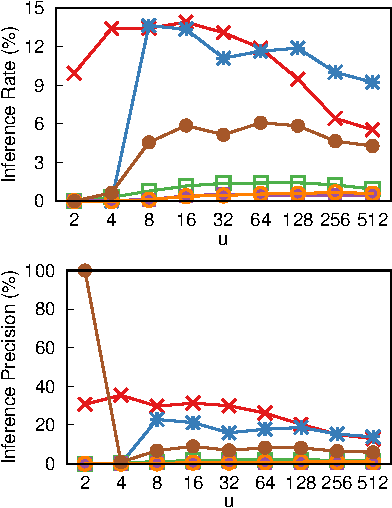
\includegraphics[width=.3\textwidth]{pic/distribution-impact-u.pdf} &
        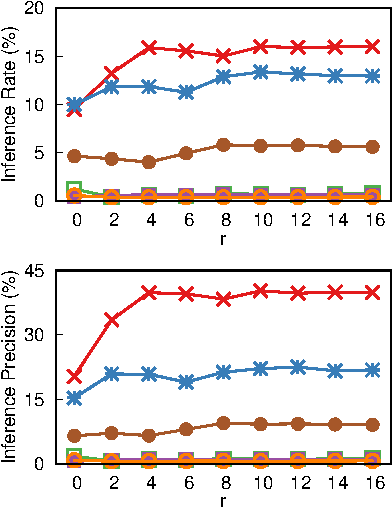
\includegraphics[width=.3\textwidth]{pic/distribution-impact-r.pdf} &
	    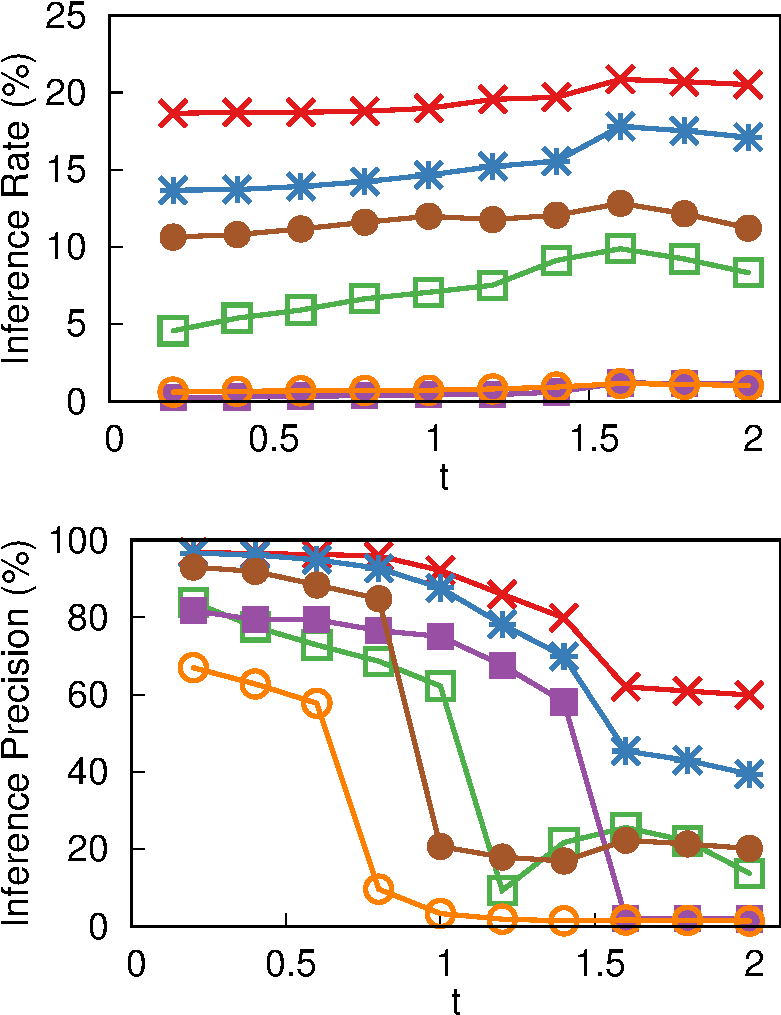
\includegraphics[width=.3\textwidth]{pic/distribution-impact-t.pdf} \medskip \\
        {\footnotesize 
        \centering
        (a) Impact of $u$: $r$ = 0; $t \rightarrow \infty$
        } &
        {\footnotesize
        (b) Impact of $r$: $u$ = 128 for User004, User013 and User015, and $u$ = 256 for User007, User012 and User028; $t \rightarrow \infty$
        } &
        {\footnotesize
        (c) Impact of $t$: $u$ = 128 for User004, User013 and User015, and $u$ = 256 for User007, User012 and User028; $r$ = 10
        } \\
    \end{tabular}
    \caption{Experiment 1 (Impact of parameters): impact of $(u, r, t)$ in distribution-based attack.}
    \label{fig:distribution-impact}
\end{figure*}


\paragraph{Experiment 1 (Impact of parameters):}
We evaluate the impact of the parameters $(u, r, t)$ in the distribution-based
attack. We drive our evaluation using the FSL dataset, and use the 12th weekly
backup of each user as the auxiliary information to infer original plaintexts
in corresponding 14th weekly backup.  We configure $t \rightarrow \infty$ and $r$ = 0 to
evaluate the impact of $u$ (in this case, the distribution-based attack
reduces to the locality-based attack \cite{li17}). Our rationale is to avoid
the disturbances by other parameters. 

Figure~\ref{fig:distribution-impact}(a) shows the impact of $u$,
when we vary $u$ from 2 to 512. Regarding inference rate, we have the same
observation as the prior work \cite{li17}. Specifically, the inference rates
first increase with $u$, since the attack can infer more ciphertext-plaintext
pairs. After hitting the maximum values (e.g., 13.9\% for User004, 13.6\% for
User007, 1.4\% for User012, 0.5\% for User013, 0.7\% for User015, and 6.1\%
for User028), they decrease.  The reason is that the underlying frequency
analysis introduces a large number of false positives that compromise the
inferences over corresponding neighbors.    

The prior work \cite{li17} does not report the inference precision about the
attack. We observe that the inference precisions for all users are at a
fairly low level (e.g., less than 40\%), except the case of $u = 2$ for
User028 that does not introduce any false positives. On the other hand, the
inference rate in the special case is about 0.0001\%, meaning that the attack
only infers a few ciphertext-plaintext pairs. In addition, as $u$ increases,
the inference precisions decrease slightly. For example, when $u$ increases
from 2 to 512, the inference precision of User004 drops from 30.7\% to 12.8\%.      

{\bf Observation (1) --} {\em A relatively larger $u$ increases the inference
rate, yet it decreases the inference precision (i.e., more false positives are
introduced). }

Informed by the impact of $u$, we set $u$ at 128 for User004, User013 and
User015, and at 256 for User007, User012 and User028, respectively, in order
to evaluate the impact of $r$ and $t$. 
% {\bf Note that the configuration
% exceeds the best one that leads to the highest inference rate. PC: I don't
% quite understand???} 
Our rationale is to increase the coverage of inferred ciphertext-plaintext
pairs, while we use $r$ and $t$ to filter possibly false positives. 

We first configure $t \rightarrow \infty$ and evaluate the impact of $r$. Figure~\ref{fig:distribution-impact}(b) shows the results. We observe that the
inference rates of majority users increase with $r$. For example, when we vary
$r$ from 0 to 16, the inference rates grow from 9.5\% to 16.0\%, from 10.0\%
to 13.0\%, from 0.5\% to 0.7\%, and from 4.7\% to 5.6\% for User004, User007,
User013, and User028, respectively. The reason is that the distribution-based
attack addresses disturbances to frequency ranking, and infer more correct
ciphertext-plaintext  pairs. On the other hand, the inference rates decrease
slightly from 1.3\% to 0.8\% and from 0.6\% to 0.4\% for User012 and User015,
respectively. The reason is that they examine a large range of plaintexts and
may introduce more false positives. In addition, the inference precisions for
all users are  at a low level (e.g., less than 45\%), and have similar
tendencies with corresponding inference rates.  

{\bf Observation (2) --} {\em A larger $r$ provides more opportunities of
identifying correct ciphertext-plaintext pairs, yet it also increases the
probability of having false positives.}   

Then, we fix $r$ = 10 and evaluate the impact of $t$. 
Figure~\ref{fig:distribution-impact}(c) shows the results. When $t$ is small
(e.g., less than 0.5), we observe that the attack misjudges and filters a
significant number of ciphertext-plaintext pairs, even they are correct. This
introduces {\em false negatives} that reduce the inference rate. As $t$
increases, the number of false negatives decreases.  When $t$ = 1.5, the
inference rates hit the maximum values at 21.2\%, 18.2\%, 10.4\%, 1.2\%,
1.2\%, and 13.5\% for User004, User007, User012, User013, User015, and
User028, respectively. When $t$ further increases to 2, the corresponding
inference rates drop to 20.5\%, 17.1\%, 8.3\%, 1.2\%, 1.0\%, and 11.2\%,
respectively. The reason is that if $t$ is too large, it cannot filter false
positives effectively. For the same reason, the inference precisions for all
users decrease with $t$.  
% The inference rates first  increase with $t$, since the number of false negatives (i.e., misjudge some correctly inferred ciphertext-plaintext pairs in filtering) are reduced.  

% implies that the distribution-based attack  returns more incorrect ciphertext-plaintext chunk pairs, which affects attack severity.  


{\bf Observation (3) --} {\em A smaller $t$ filters a large fraction of false
positives, yet it introduces more false negatives.}   


\paragraph{Experiment 2 (Comparison with prior attack):}
We compare the severity of the distribution-based attack with that of the
locality-based attack \cite{li17}. In addition to using the FSL dataset like
Experiment~1, we include the MS dataset for cross-dataset validation.
Specifically, for each MS category, we choose two snapshots at a time, use one
to infer the other, and evaluate the average inference rate and precision. 

We consider the following attack instances for comparison. 
%
\begin{itemize}[leftmargin=*]
\item 
$\tt Baseline$: We re-implement the locality-based attack based on the
parameter configuration suggested in \cite{li17}. Specifically, it infers 5
most frequent ciphertext-plaintext pairs in the first invocation (i.e., to
initialize a set of ciphertext-plaintext pairs for iteration) of frequency
analysis, and 30 in each following invocation (i.e., to iteratively infer ciphertext-plaintext pairs from 
 neighbors).  
\item 
$\tt Distribution$ and $\tt Distribution^S$: We consider two attack instances
of the distribution-based attack, denoted by $\tt Distribution^S$ and ${\tt
Distribution}$, which operate with and without size information,
        respectively (i.e., the superscript $\tt S$ indicates that the attack instance operates with size information). 
        We configure $\tt Distribution^S$ and ${\tt Distribution}$
under the same configuration of  ${\tt Baseline}$. In addition, we choose
$r$ and $t$ in both  $\tt Distribution^S$ and ${\tt Distribution}$ in the following way: for the FSL dataset, we fix $r$ = 10 for
all users, and individually set $t$ = 1.5, 1.2, 1, 1, 0.7, and 0.9 for
User004, User007, User012, User013, User015, and User028, respectively; for
the MS dataset, we also fix $r$ = 10 for all categories, and set $t$ = 2 for
Win7 and Serv-08, and $t$ = 1.6 for Vista-U, Serv-03, and Vista-B, respectively.
This is informed by our tests for optimal configurations of the datasets.   
\item 
$\tt Distribution$-$\tt o$ and $\tt Distribution^S$-$\tt o$:
We consider two additional distribution-based attack instances, denoted by $\tt Distribution$-$\tt o$
and $\tt Distribution^S$-$\tt o$, which apply the same configurations for $r$ and $t$ as with $\tt Distribution$ and $\tt
Distribution^S$, and further use larger $u$ to increase the
coverage of inferred ciphertext-plaintext pairs.  
        Specifically, we configure $u$ in $\tt Distribution$-$\tt o$
and $\tt Distribution^S$-$\tt o$ in the following way:  
        for the FSL
dataset, we apply the same configuration of $u$ in Experiment~1; for the MS
dataset, we set $u$ = 128 for Win7, and $u$ = 30 for Serv-03, Serv-08,
Vista-B, and Vista-U. 
        % Our rationale is to increase
% the inference rate, while we expect  this only leads to a slight
% degradation of the inference precision since the distribution-based attack
% filters a large fraction of false positives. 
\end{itemize}

\begin{figure*}[t]
    \centering
    \begin{tabular}{c@{\hskip 2em}c}
        \multicolumn{2}{c}{
\includegraphics[width=.7\textwidth]{pic/legend-fsl-bar.pdf}} \smallskip \\
        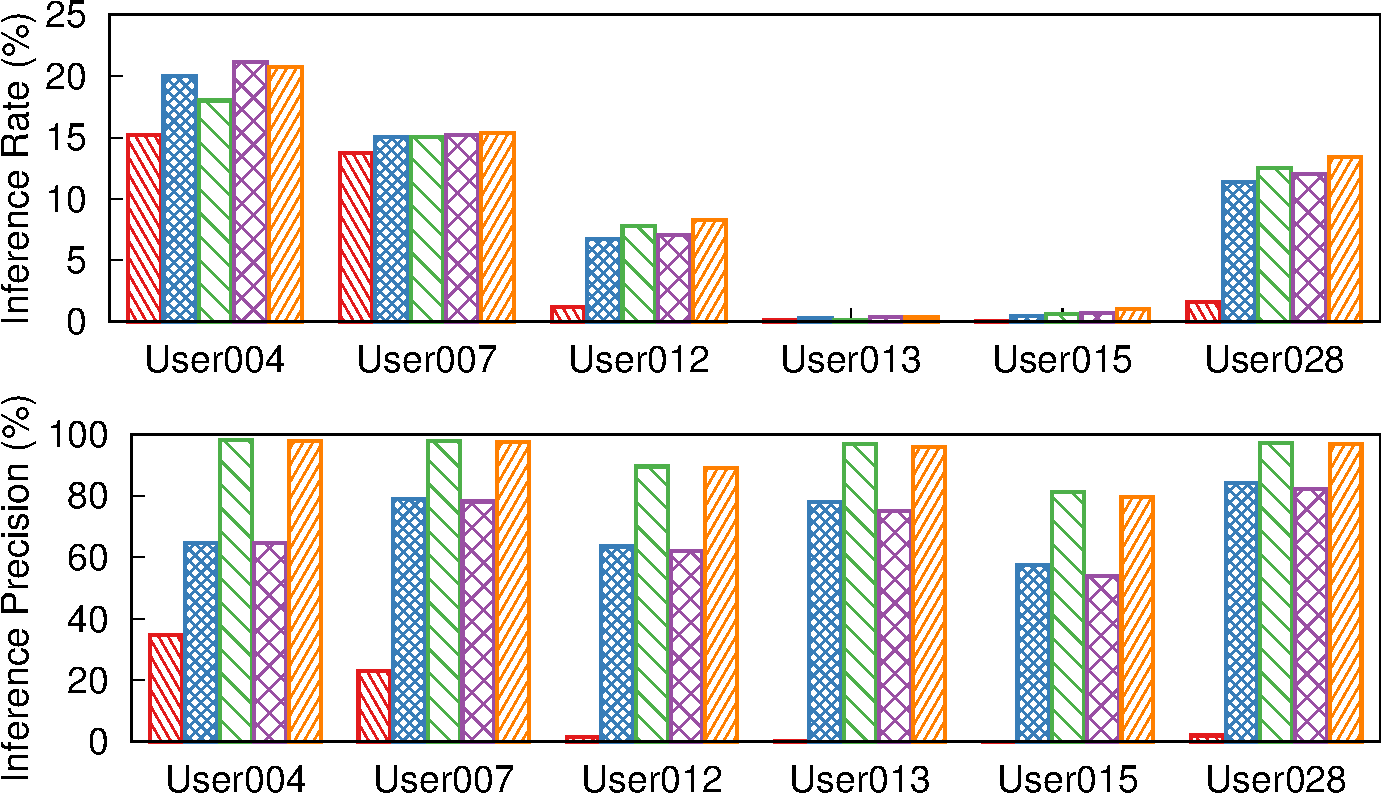
\includegraphics[height=2.1in]{pic/distribution-comparison-fsl.pdf} &
        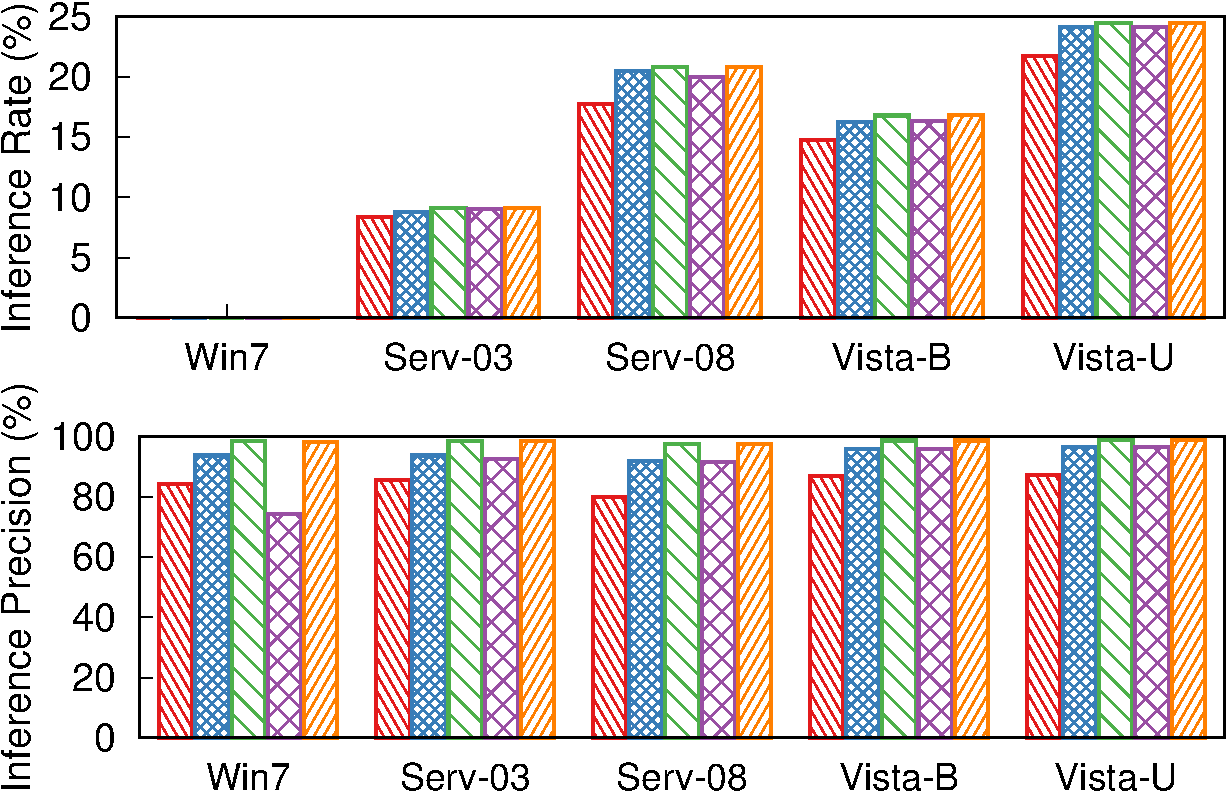
\includegraphics[height=2.1in]{pic/distribution-comparison-ms.pdf} \medskip \\
        {\footnotesize 
        (a) FSL dataset 
        } &
        {\footnotesize
        (b) MS dataset 
        } \\
    \end{tabular}
    \caption{Experiment 2 (Comparison with prior attack): comparison of attack severity for distribution-based attack and locality-based attack.}
    \label{fig:distribution-comparison}
\end{figure*}



% \begin{itemize}[leftmargin=*]
	% \item {\em Distribution-I:} We configure our proposed distribution-based attack with the {\em same} configuration of the baseline above. Informed by Experiment 3, we further choose the distribution-based ranking parameters in the following way: for the FSL dataset, we fix $r$ = 10 for all users, and individually set $t$ = 1.5, 1.2, 1, 1, 0.7, and 0.9 for User004, User007, User012, User013, User015, and User028; for the MS dataset, we fix $r$ = 10 for all categories, and configure $t$ as 2 for Win7 and Serv-08 and as 1.6 for Vista-U, Serv-03, and Vista-B, respectively.   

	% \item {\em Distribution-II:} We configure our proposed distribution-based attack with the same ranking configuration of distribution-I, while building on a larger $u$ to infer more chunk pairs. The rationale is to increase inference rate, while we expect the inference precision is degraded slightly as the attack can filter out unreasonable inferences. Specifically, for the FSL dataset, we set $u$ = 128 for User004, User013 and User015, and $u$ = 256 for User007, User012 and User028, respectively; for the MS dataset, we set $u$ = 128 for Win7, and $u$ = 30 for Serv-03, Serv-08, Vista-B, and Vista-U, respectively.
% \end{itemize}

Figure~\ref{fig:distribution-comparison}(a) shows the
comparison results of the FSL dataset. We observe that different instances of
the distribution-based attack outperform the locality-based attack in almost
all cases. For example, regarding User028, the lowest inference rate of the
distribution-based attack is 11.4\%, with the precision of 84.1\% (due to $\tt
Distribution$), while the corresponding inference rate and precision of
$\tt Baseline$ are only 1.2\% and 1.7\%, respectively; this implies that the distribution-based attack reduces the number of false postives by 82.4\% in this case.   

{\bf Observation (4) --} {\em The distribution-based attack significantly
increases the inference precision, while achieving a higher inference rate than
the locality-based attack.} 

$\tt Distribution^S$ and $\tt Distribution^S$-$\tt o$ have higher inference
precisions than $\tt Distribution$ and $\tt Distribution$-$\tt o$,
respectively, since they further filter false positives by size information.
For example, for User004, $\tt Distribution^S$ and $\tt Distribution^S$-$\tt o$  reduce the fraction of false positives in  $\tt Distribution$ and $\tt Distribution$-$\tt o$ from 35.2\% to 1.7\% and from 35.3\% to 2.2\%, respectively. However, in the same case,    
 we observe that the inference rates of $\tt Distribution$ and $\tt Distribution$-$\tt o$ are 20.0\% and 21.2\%, slightly higher than those of  
$\tt Distribution^S$ and
$\tt Distribution^S$-$\tt o$ by 2.0\% and
0.4\%, respectively. The reason is that $\tt Distribution$ and $\tt
Distribution$-$\tt o$ infer a small number of correct results from the
neighbors of incorrect ciphertext-plaintext pairs. In other words,  although
$(C, M)$ is an incorrect ciphertext-plaintext pair, the neighbors of $C$ may
correspond to those of $M$ with a small probability. Even in this case, all distribution-based attack instances are more severe than the locality-based attack instance. Specifically, the inference rate of $\tt Baseline$ is only 15.2\%, lower than those of the best and the worst distribution-based attack instances by 6.0\% and 2.8\%, respectively. 

% For the same reason, $\tt Baseline$ has higher inference rate than $\tt Distribution^S$ in User013.   

{\bf Observation (5) --} {\em Filtering incorrect inference results improves
the inference precision, yet it degrades the coverage of inferred
ciphertext-plaintext pairs and possibly decreases the inference rate.
} 

We further observe that although $\tt Distribution$-$\tt o$ and $\tt
Distribution^S$-$\tt o$ build on larger $u$, their inference rates are just
slightly higher than those of $\tt Distribution$ and $\tt Distribution^S$ by
0.4\% and 0.9\%, respectively. The reason is that the distribution-based
attack iterates inference just through neighbors, and has a bounded coverage
of inferred ciphertext-plaintext pairs. The further increase of $u$ only adds
a small number of new correct  ciphertext-plaintext pairs into results. 

Figure~\ref{fig:distribution-comparison}(b) shows the
results of the MS dataset. Both locality-based and distribution-based attacks
have high inference rates and precisions in most MS categories (except Win7).
The possible reason is that MS snapshots are highly correlated (e.g., the
variance of the total number of chunks is small, as shown in
Table~\ref{tab:dataset}).  We observe that the distribution-based attack still
outperforms the locality-based attack. For example, in Vista-U, the inference
rates and precisions of all inferences of the distribution-based attack are
above 24.1\% and 96.4\%, while those of $\tt Baseline$ are 21.7\% and 87.1\%,
respectively. 

Note that both  distribution-based and  locality-based attacks have low
inference rates (e.g., less than 0.01\%) in the Win7 category. The reason is
 that Win7 includes a large fraction (e.g., more than 98.8\%, as shown in
Table~\ref{tab:dataset}) of unique chunks, which cannot be correctly
inferred by the frequency analysis attacks. 

% We do not include Win7  in the comparison, since all attack instances have low effectiveness. We observe all attacks have higher severity than those in the FSL dataset.   



\begin{figure*}[t]
     \centering
    \centering
    \begin{tabular}{c@{\hskip 2em}c}
        \multicolumn{2}{c}{
\includegraphics[width=.25\textwidth]{pic/legend-effectiveness.pdf}} \smallskip \\
        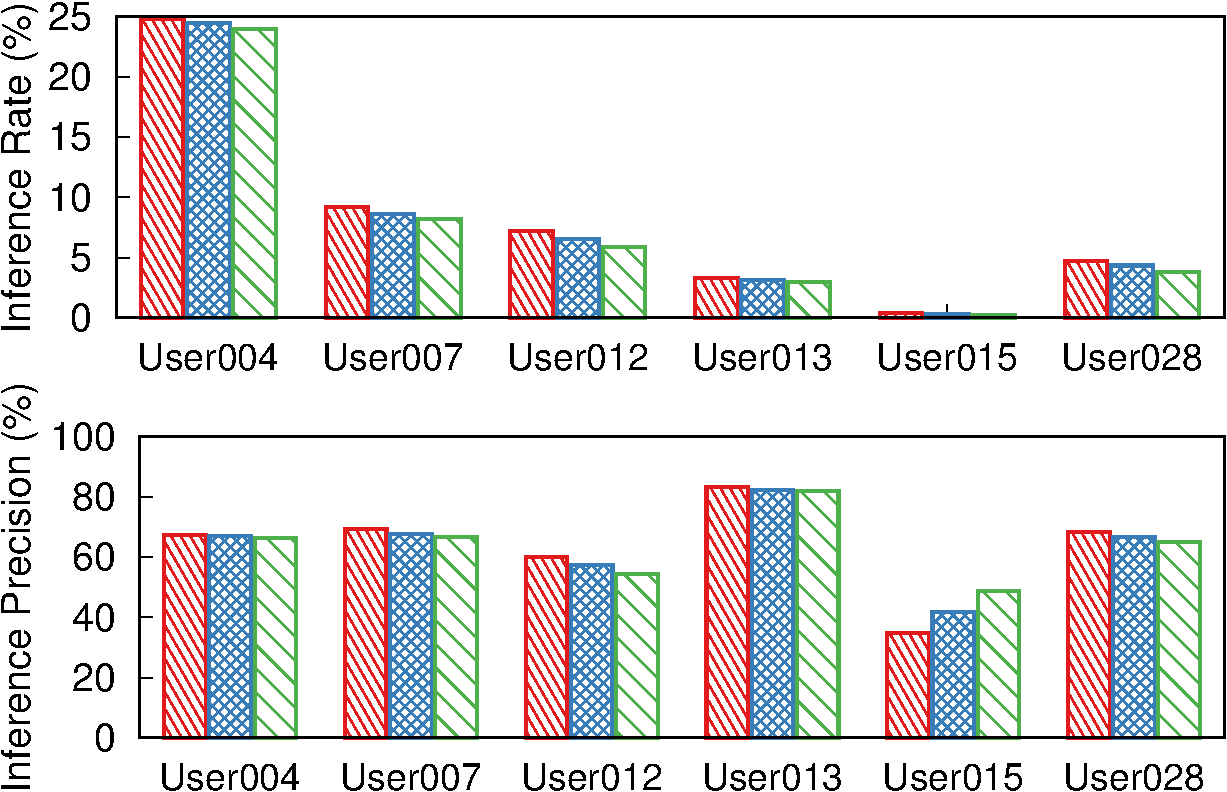
\includegraphics[height=2.2in]{pic/distribution-effectiveness-wo-size.pdf} &
	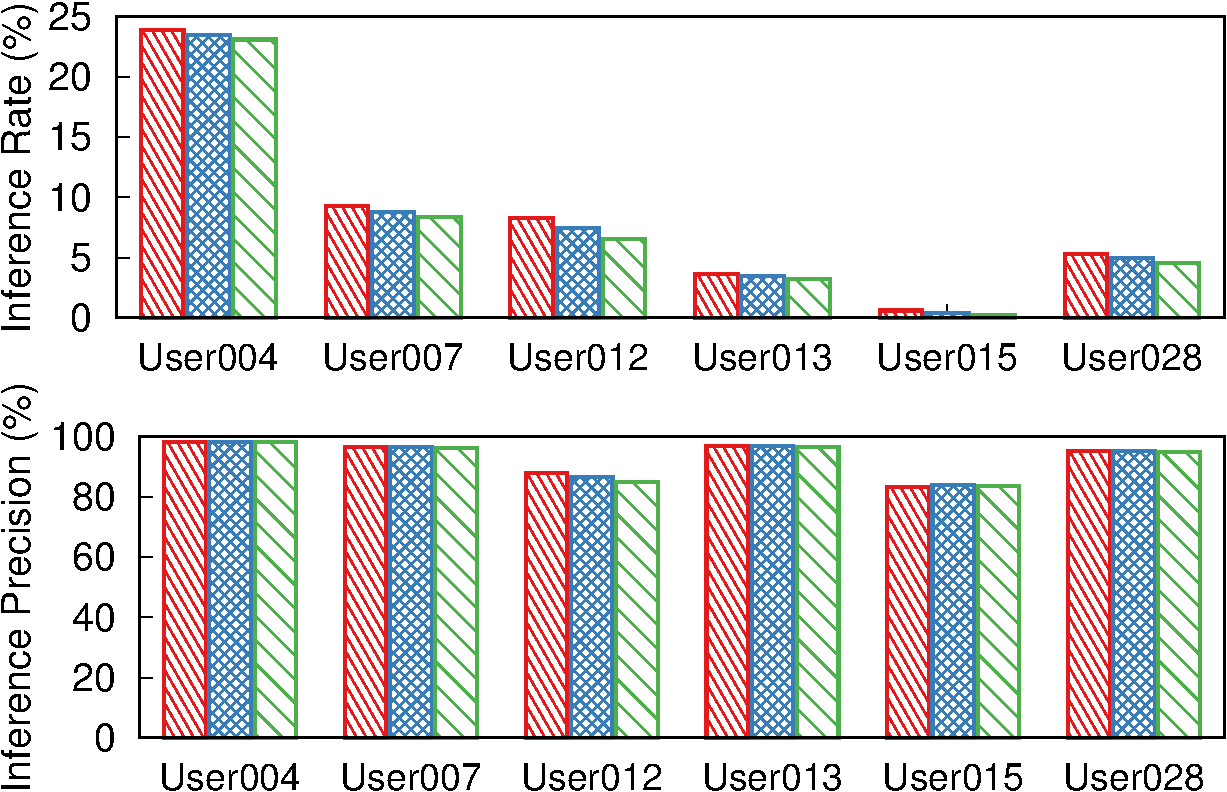
\includegraphics[height=2.2in]{pic/distribution-effectiveness-w-size.pdf} \medskip \\
        {\footnotesize 
        (a) Distribution-based attack without size information  
        } &
        {\footnotesize
        (b) Distribution-based attack with size information 
        } \\
    \end{tabular}
	\caption{Experiment 3 (Attack effectiveness): severity of distribution-based attack in FSL dataset.}
	\label{fig:experiment-distribution-effectiveness}
\end{figure*}


\paragraph{Experiment 3 (Attack effectiveness):} We consider a long-term
backup scenario and examine the effectiveness of the distribution-based attack
with the FSL dataset. Specifically, we choose the $i$th FSL weekly backup of
each user as the auxiliary information to infer original plaintexts in the corresponding $(i+w)$th FSL
weekly backup. Clearly, the smaller $w$ is, the higher correlation between the
auxiliary information and the target backup will be.  We configure the two  
distribution-based attack instances $\tt Distribution$-$\tt o$ and $\tt Distribution^S$-$\tt o$
like Experiment~2, and evaluate their inference rates and inference precisions that
are averaged for all available $i$ for each user. 

Figure~\ref{fig:experiment-distribution-effectiveness}(a) shows the results. The
distribution-based attack has varying inference rate and precision  across
users. For example, in the favorable case like User004, it achieves the
highest inference rates of 24.8\%, 24.5\%, and 24.0\% with the precisions of
67.3\%, 67.0\%, and 66.5\% for $w$ = 1, 2, and 3, respectively; in the
non-favorable case like User015, the inference rate of the distribution-based
attack is only around 0.3\%. The possible reason is that the backup data from
User015 has low chunk locality. 

In addition, we observe that the correlation (i.e., $w$) of the auxiliary
information has low impact on the effectiveness of the distribution-based
attack.  For example, when $w$ increases from 1 to 3, it only leads to limited
degradations on inference rate (e.g., less than 1.4\%) and precision (e.g.,
less than 5.6\%). The reason is that the distribution-based attack addresses
disturbances to frequency ranking and preserves attack effectiveness.  

{\bf Observation (6) --} {\em The distribution-based attack can limit the
degradation of attack effectiveness in the presence of loosely correlated
auxiliary information.} 

% We also use the instance in Experiment 2 to evaluate the effectiveness of the distribution-based attack that operates with
 % size information. 
 Figure~\ref{fig:experiment-distribution-effectiveness}(b) shows the results of $\tt Distribution^S$-$\tt o$. We observe that it has similar inference rate with $\tt Distribution$-$\tt o$,  
 while achieving much higher precision. For example, the average inference precision of all users are 93.1\%, 92.8\%, and 92.4\% for $w$ = 1, 2, and 3, respectively.  

% Figure~\ref{fig:experiment-distribution-severity-ms} shows the attack results of the MS dataset. The distribution-based attack achieves high severity. For example, it can infer 24.0\% of unique chunks in Vista-U with a precision of 96.2\%.    

% Although there is l          

\section{Results of Clustering-based Attack}
\label{sec:experiment-clustering}




\paragraph{Experiment 4 (Impact of parameter):} We first evaluate the impact
of the parameter $k$, which defines the upper bound distance
in combining the closest clusters.  We use both the FSL and the VM datasets to
study how $k$ affects the underlying clustering scheme in the attack.
Specifically, we apply segmentation on the last backup of each considered FSL
and VM user, respectively, and generate the segments that have a fixed size of
4MB. 

The clustering scheme aims to aggregate similar ciphertext segments into the
same cluster, without compromising the confidentiality of chunks in each
ciphertext segment.  To quantify its effect, we compare the results of
clustering with those of a {\em real} classification approach, which directly
classifies segments by their minimum chunk hash.  Suppose we generate $m$ real
classes of segments by classification, and $\widetilde{m}$ clusters by the
clustering scheme, respectively.  We consider {\em clustering closeness},
evaluated by $\frac{{\sf abs}(m-\widetilde{m})}{m}$ (where 
${\sf abs}(m-\widetilde{m})$ returns the absolute value of $m-\widetilde{m}$),
which quantifies how the  number of clusters approximates that of real
classes. In addition, let $\hat{m}$ be the number of clusters, in which all
segments are similar (i.e., have the same minimum chunk hash). We also
consider {\em clustering correctness}, evaluated by
$\frac{\hat{m}}{\widetilde{m}}$, which quantifies how precisely the clustering
scheme groups similar segments.  

Figure~7(a) shows the results of the FSL dataset, where we
consider four FSL users (e.g., User004, User007, User015 and User028) for
saving evaluation time. The clustering closeness first increases with $k$,
since the number (i.e., $\widetilde{m}$) of clusters decreases and
approximates $m$. When $k$ increases further, the number of clusters drops
away from $m$, and leads to the increase of clustering closeness.  In
addition, we observe that the clustering correctness gradually decreases with
$k$, because some of non-similar segments (i.e., their minimum chunk hashes are
different) are aggregated into the same cluster. Both results suggest that we
can configure an appropriate $k$ to balance the closeness and correctness of
clustering. For example, when we set $k$ = 0.65 for User015, the corresponding
closeness and correctness are 1.0\% and 94.2\%, respectively. This implies
that the results of the clustering scheme  highly approximates
those of real classification.             

{\bf Observation (7) --} {\em By configuring an appropriate $k$ for
clustering, we  approximate the results of  classifying segments, without the knowledge of  minimum chunk hash in each
segment.}   

Figure~7(b) shows the results of the VM dataset. We observe
that the clustering closeness and correctness of all VM users have  similar
tendencies with those of FSL users. When we configure $k$ = 0.8, the average
clustering closeness of all VM users is only 3.0\%, while the corresponding
clustering correctness is as high as 93.1\%.     


\begin{figure*}[t]
\centering
    \begin{tabular}{cc@{\hspace{0.3in}}p{.32\textwidth}}
    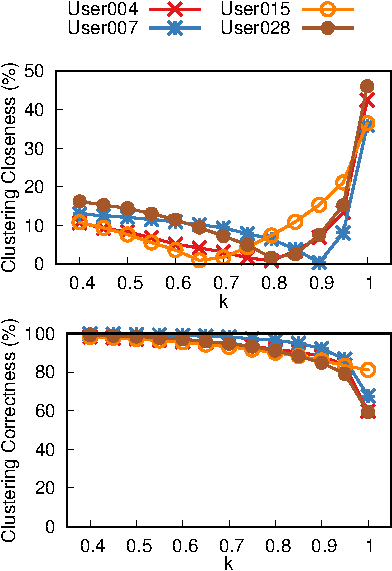
\includegraphics[width=.3\textwidth]{pic/clustering-impact-d-fsl.pdf} &
    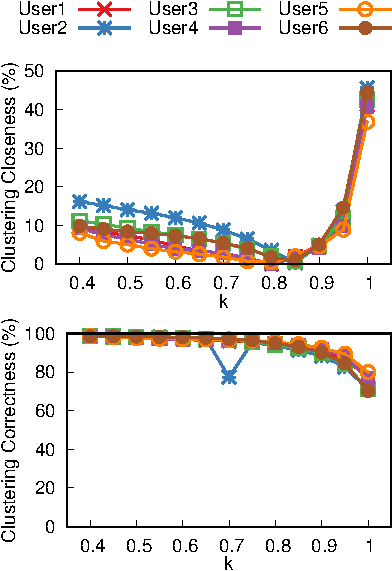
\includegraphics[width=.3\textwidth]{pic/clustering-impact-d-vm.pdf} & 
    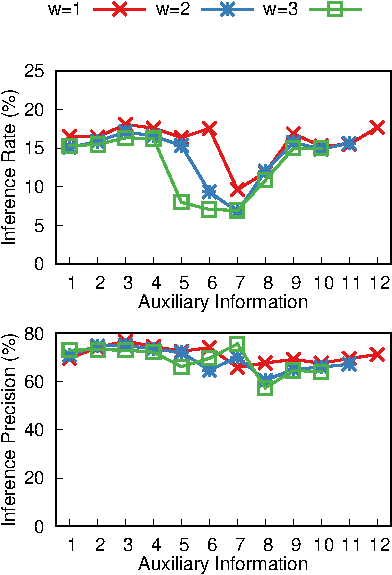
\includegraphics[width=.3\textwidth]{pic/clustering-effectiveness.pdf} \medskip \\
{\footnotesize 
        (a) FSL dataset } 
&
{\footnotesize 
        (a) VM dataset } 
        &  ~~~ \medskip \\
        \multicolumn{2}{p{.64\textwidth}}{
            \footnotesize Fig.~7\quad Experiment 4 (Impact of parameter): impact of $k$ in the clustering scheme; for clustering closeness, the smaller the better; for clustering correctness, the larger the better. } &
        % \multicolumn{2}{c}{\footnotesize Fig.~6\quad Experiment 4 (Impact of parameter): show impact of $d$ with clustering closeness and correctness; for clustering closeness, the smaller the better; for clustering correctness, the larger the better.} &
        {\footnotesize
Fig.~8\quad Experiment 5 (Attack effectiveness):  severity of clustering-based attack in VM dataset.
        }
\end{tabular}
    \hspace{-1in}
\end{figure*}

% \begin{figure}
% 	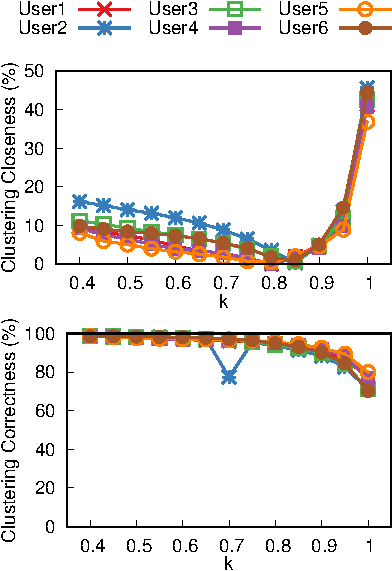
\includegraphics[width=.48\textwidth]{pic/clustering-impact-d.pdf}
% 	\caption{Experiment 6 (Impact of parameter).}
% 	\label{fig:experiment-clustering-impact}
% \end{figure}

\begin{table*}[!t]
\small
    \caption{Experiment 6 (Security implications)}
\renewcommand{\arraystretch}{1.2}
\vspace{-3pt}
 \begin{minipage}[t]{0.7\textwidth}
\centering
        (a) Distribution-based attacks \medskip \\
\begin{tabular}{|c|c|c|c|c|c|}
\hline

    \multirow{2}{*}{\bf Type} & \multirow{2}{*}{\bf Extension Name} & \multirow{2}{*}{\bf \centering Range of File Size}  & \multicolumn{2}{c|}{\bf Raw Inference Rate} \\ \cline{4-5} 
    & & &  $\sf Distribution$-$\sf o$ & $\sf Distribution^S$-$\sf o$ \\ \hline
\hline
    Office & doc(x), ppt(x), xls(x) & 10KB-1MB   & 4.9\% & 5.3\%\\
\hline
    Picture & jpg, png &10-100KB  & 7.7\% & 6.7\% \\
\hline
    Source & c, h, cpp, java, py & 10-20KB   & 17.1\% & 15.0\%\\
% \hline
	% Library & .a, .dll, .so \\
% \hline
	% Compression & .bz2, .gz, tar, rar, zip, 7z \\
\hline
    Database & db, po & 20-700KB   & 2.6\% & 2.4\%\\
\hline
    Disk & vmdk, img & 200MB-1GB  & 15.8\% & 16.7\%\\
\hline
\end{tabular}
\label{tab:file}
 \end{minipage}
\hfill
    \begin{minipage}[t]{0.3\textwidth}
    \centering
        (b) Clustering-based attack \medskip \\
    \begin{tabular}{|c|c|}
    \hline
        {\bf Users} & {\bf Raw Inference Rate} \\
    \hline
    \hline
        1 & 13.2\% \\ 
    \hline
        2 & 22.4\% \\ 
    \hline
        3 & 25.7\% \\ 
    \hline
        4 & 28.4\% \\ 
    \hline
        5 & 18.5\% \\ 
    \hline
        6 & 30.8\% \\ 
    \hline
    \end{tabular}
\label{tab:user}
    \end{minipage}

\end{table*}



\paragraph{Experiment 5 (Attack effectiveness):} We now study the
effectiveness of the clustering-based attack. Due to the boundary shift of
fixed-size segment, it has low effectiveness
(about 1\% inference rate in our test) against the FSL dataset.  Thus, we use
the VM dataset to examine its severity. To configure the attack, we set $k$ =
0.8 for clustering, and $(u, r, t)$ = (5000, 100, 0.5) for relating ciphertext
clusters to corresponding plaintext clusters.  

In our micro-benchmarking, we find that the chunk-level inference in the
clustering-based attack only infers thousands of chunks correctly, which
contributes to a negligible inference rate (e.g., less than 0.01\%).  
% The
% reason is that each cluster includes a large number of chunks, and frequency
% analysis is ineffective in this case. 
Thus, we focus on the
segment-level inference, which presents the bottom line of severity in the
clustering-based attack. To be consistent with the chunk-level measurements, we count inference rate and precision based
on the unique chunks in each correctly inferred segment. 

We use the same evaluation methodology of Experiment~3, and report the results
in Figure~8. Specifically, the x-axis describes the index $i$ (where 1 $\leq i \leq$
12) of the VM backup that is used as the auxiliary information for attack,
while the y-axis presents the average inference rate or precision of all VM
users against the $(i+w)$th backup (where $w$ = 1, 2, and 3). We observe that both the inference rate and the inference
precision fluctuate significantly. For example, when using the 3rd backup as
the auxiliary information, the attack achieves the highest inference rates at
18.1\%, 17.1\% and 16.3\%, with the precisions of 76.8\%, 75.0\% and 73.0\%
for $w$ = 1, 2, and 3, respectively. 
On the other hand, when using the 7th
backup as the auxiliary information, the corresponding inference rates and
precisions drop down to 9.6\% and 65.9\%, 6.8\% and 71.2\%, and 6.9\% and
75.6\%, respectively. The reason is that the VM users have heavy updates after
the 7th week, and this reduces the correlation  of adjacent backups. 
On
average, for $w$ = 1, 2 and 3, the clustering-based attack infers 15.8\%,
14.0\%, and 12.6\% ciphertext-plaintext pairs, with the precisions of 71.1\%,
69.1\%, and 68.9\%, respectively. 
% This demonstrates high severity against
% the VM disk images.   

\section{Results of Security Implications}
\label{sec:case}
We thus far have examined the severity of inference attacks by quantifying the
correctly inferred ciphertext-plaintext pairs.  However, it remains an open
issue that what are the security implications informed by these results and
how the frequency analysis attacks bring actual damage. In the following
experiment, we evaluate the security implications of our attacks based on the
{\em raw inference rate}, defined as the percentage of raw data content
affected by correctly inferred chunks.   




\paragraph{Experiment 6 (Security implications):}
We first consider the distribution-based attack, and evaluate its raw
inference rate against {\em different types} of files. We drive the evaluation
using the FSL dataset, since only the FSL dataset includes file metadata (that
includes the extension names of files) in plaintext. Specifically, we focus on
five types of files that have specific extension names (see
Table~\ref{tab:file}(a)): office files ({\em Office}), picture files 
({\em Picture}), programming source files ({\em Source}), database files 
({\em Database}), and disk image files ({\em Disk}). These files occupy more
than 60\% of raw content of FSL snapshots.   

We apply the methodology of Experiment~2, and evaluate the raw inference
rates of $\sf Distribution^S$-$\sf o$ and $\sf Distribution$-$\sf o$. 
Table~\ref{tab:file}(a) shows the results. Both attack instances have high raw
inference rates against {\em Disk} (e.g., 15.8\% for 
$\sf Distribution$-$\sf o$ and 16.7\% for $\sf Distribution^S$-$\sf o$),
because each disk file includes a large number of rarely updated chunks that
form high locality within the same file. Interestingly, we observe that 
{\em Source}, although each file is of a small size, also incurs high raw
inference rates by the distribution-based attacks (e.g., 17.1\% for 
$\sf Distribution$-$\sf o$ and 15.0\% for $\sf Distribution^S$-$\sf o$). The
reason is that programming source files are often stored together in file system
(e.g., the source files that belong to the same project locate in an identical
directory) and form a large stretch of correlated chunks, which present high
locality across files. For small and scattered files (e.g., {\em Office}, 
{\em Picture}, and {\em Database}), the distribution-based attacks have
relative low raw inference rates.     


{\bf Observation (8) --} {\em The severity of the distribution-based attack depends on the update frequencies, sizes, and spatiality of target files. } 

We examine the security implication of the clustering-based attack using the
VM dataset. Specifically, we use the 11th  backup of each VM user  to infer original content in corresponding 13th VM
backup. Since the VM dataset does not contain any metadata, we count the raw
inference rate based on the  whole data content in each VM snapshot.
Note that we filter all zero chunks in the count of raw inference rate,
because they occupy a large fraction in VM disk images \cite{jin09}.           


% switch to the clustering-based attack, and infer the content of the last (i.e., the 13th) VM backup based on the corresponding 11th backup. Since the VM dataset does not contain metadata, we evaluate the raw inference rate across different users. Specifically, like Experiment 7, we only consider segment-level attack for high precision, and count the raw inference rate based on the correctly inferred segments. Note that since VM images commonly contain a large fraction of zero chunks ,  we filter out the zero segments in our inferred raw content.    

We use the same configuration of Experiment~5, and evaluate raw inference rate
based on segment-level inference.  Table~\ref{tab:user}(b) shows the results
for different users.  We observe that the clustering-based attack achieves high
severity against the VM dataset. For example, it infers up to 30.8\% raw
content of User6's VM backup. On average, the raw inference rate of all users
is as high as 23.2\%.  
% a relatively high raw inference rate.  On average, the raw inference rate is 23.2\% for all users. 

{\bf Observation (9) --} {\em The clustering-based attack threatens the
confidentiality of VM disk images. } 

\chapter{Countermeasure Discussion}
\label{sec:countermeasure}

In this section, we discuss the advantages and disadvantages of possible countermeasures against the leakage channels exploited in this paper. Note that the countermeasures against size leakage are not enough for preventing our attacks, in which the size information is just optional.  

\paragraph{Against frequency leakage:}
MinHash encryption \cite{qin17, li17} encrypts each plaintext with a key derived from the minimum chunk hash over a set of its adjacent chunks, and possibly maps identical plaintexts into  different ciphertexts. The rationale for defense is that MinHash encryption changes frequencies, and disturbs frequency ranking. 
 Note that MinHash encryption also prevents the frequency analysis attacks in this paper, because  we target deterministic encryption (e.g., MLE \cite{bellare13a}), while MinHash encryption is non-deterministic and changes the  frequency distribution of chunks. The disadvantage is that MinHash encryption degrades the storage saving by deduplication, since it breaks the one-to-one mapping between plaintexts and ciphertexts. In addition, MinHash encryption is not an active countermeasure, since its randomness essentially depends on the minimum chunk hashes in the target workloads.            




% (rather than the chunk itself \cite{bellare13a}) over its adjacent chunks, so that some identical plaintext chunks can be encrypted into different ciphertext chunks. The rationale of defense is MinHash encryption {\em changes the frequencies of chunks} and leads to rank disturbances in classical frequency analysis. In addition, the nature of MinHash encryption is {\em non-deterministic}, and prevents the distribution-based ranking (see \S\ref{sec:distribution-attack-description}) that targets deterministic encryption. On the other hand, MinHash encryption is not an {\em active} countermeasure, since its defense effectiveness is dominated by workload characteristics (i.e., depending on the diversity of MinHash). It also degrades deduplication effectiveness due to breaking the one-to-one mapping between plaintexts and ciphertexts.

A recent work \cite{zuo18} suggests intentionally adding duplicate chunks to prevent traffic analysis against client-side deduplication. The approach \cite{zuo18} can be applied to address the frequency analysis attacks, since it changes the frequencies of chunks. Compared with MinHash encryption, the countermeasure \cite{zuo18} does not degrade storage efficiency, since only duplicate chunks are added. On the other hand, it  requires the priori knowledge that if particular chunks are duplicate, and only suits the client-side deduplication, which possibly introduces additional leakage channels (see Section~\ref{sec:related}).  

Several extended MLE instantiations build on strong cryptographic primitives to defend against the frequency leakage of encrypted deduplication, such as randomized encryption that supports equality testing \cite{abadi13}, hybrid encryption \cite{stanek14}, and interactions with fully homomorphic encryption \cite{bellare15}. They provide provable security, yet how they can be implemented and deployed in practice remains unexplored. 

 

% yet how they are implemented and deployed in practice remains unexplored. 
% some random encryption schemes \cite{stanek14,bellare15,abadi13,lacharite18a}  address the frequency leakage of deterministic encryption. Other than the practical approaches \cite{qin17, li17, zuo18}, they provide provable security, yet building on computationally expensive primitives. 
% % (see Section~\ref{sec:related}).   


% are proposed to address frequency leakage from cryptography aspect, yet they are not readily implemented in practice .    


% Some studies \cite{stanek14,abadi13,bellare15} aim to achieve stronger security than the more practical schemes focused above. Stanek {\em et al.} \cite{stanek14} design a hybrid encryption scheme where unpopular messages are protected by semantically secure encryption for high security guarantee, while popular messages are protected by CE to enable deduplication. On the other hand, the scheme \cite{stanek14} builds on public-key primitive which is inefficient for encrypting large-size messages. Abadi {\em et al.} \cite{abadi13} construct two schemes for the messages whose distributions are publicly available. Their first scheme generates  random tags and ciphertexts to prevent frequency leakage, yet incurring expensive {\em equality test} for checking duplicates. Their second scheme produces deterministic ciphertexts, and exposes the frequencies of corresponding plaintexts. Interactive MLE \cite{bellare15} introduces interactions into encrypted deduplication, and strengthens the security of both correlated and parameter-dependent messages, yet it is impractical for the use of fully homomorphic encryption. On the contrary to these theoretical contributions \cite{stanek14, abadi13, bellare15}, this paper focuses on the applied aspect, and investigates the security vulnerabilities in practical deduplication.   

\paragraph{Against order leakage:}
A simple countermeasure is to disturb the deduplication processing sequence of chunks. For example, we can operate an additional order-scrambling process on the stream of plaintexts before encryption, so as to hide the actual logical order of each plaintext. This prevents the distribution-based attack, because the adversary cannot identify neighboring information correctly. On the other hand, it is not always effective against the clustering-based attack. If scrambling  operates on just a small basis (e.g., the orders of plaintexts in each segment are scrambled), the clustering-based attack still works. 
The disadvantage of the order-scrambling countermeasure is that it breaks chunk locality and leads to performance drop in large-scale deduplication \cite{xia11,zhu08,lillibridge09}. 


% On the other hand, if we operate scrambling        
% {\em scrambling}, which intentionally disturbs the deduplication processing sequence of chunks. 
% operates the stream  before deduplication and disturbs the order of each plaintext. 
% disturbs the orders of plaintexts before deduplication 
% to scramble the orders of plaintexts. Specifically, the scrambling approach , and randomly changes the order of each plaintext.   
% A countermeasure is to scramble the orders of chunks, so as to prevent adversary from learning the actual order of each chunk. One note is the scrambling countermeasure should be applied by taking similarity into account; otherwise, the adversary can exploit the property for inference attack (see \S\ref{sec:clustering-attack}). For example, applying scrambling in a small basis (e.g., within a segment) is not enough for preventing the clustering-based attack. On the other hand, large-scale scrambling breaks chunk locality completely, and leads to significant degradation of deduplication performance .

\paragraph{Against size leakage:}
As suggested by prior work \cite{ritzdorf16}, we can pad each plaintext with additional data to obfuscate the actual size of this plaintext. However, we note that the padding scheme is not straightforward, since it requires to add identical redundancies to the same plaintexts; otherwise the storage system cannot detect duplicates for deduplication. One possible solution is to build on the paradigm of MLE \cite{bellare13b,bellare13a}. We compute the cryptographic hash of each plaintext as a seed, and use it to generate variable-size pseudorandom data to be padded with the  plaintext. Like MLE, this solution comes at the expense of server-aided approach \cite{bellare13b} to defend against brute-force attack (see Section~\ref{sec:related}).     


% A countermeasure is to sacrifice storage efficiency and {\em pad each chunk with additional data}, which can obfuscate the original size of this chunk. The padding scheme is not straightforward, as it is required to {\em add identical redundant data to the same chunks}; otherwise, the server cannot detect duplicates for deduplication. One possible solution is based on the spirit of MLE \cite{bellare13b,bellare13a}. 
% Specifically, we compute the cryptographic hash of each chunk as a seed, and use the seed to generate variable-size pseudorandom data to be padded with the corresponding chunk. Like MLE, this solution comes at the expense of server-aided approach \cite{bellare13b} to defend against brute-force attack (see \S\ref{sec:related}).    
  
  Instead of variable-size chunking, we can use fixed-size chunking to 
 generate equal-size chunks for deduplication. Since all chunks have the same size, the adversary cannot exploit size information to differentiate them.  Although fixed-size chunking suffers from boundary shift, it achieves almost the same storage saving of deduplication as variable-size chunking in VM disk images \cite{jin09}. Thus, we suggest applying fixed-size chunking in its favorable workloads to prevent size leakage.  

      
  
  % make the leaked size information hard to be exploited for inference attack. It suffers from the shift of chunk boundaries and is less effective for majority workloads, while prior work \cite{jin09} shows fixed-size chunking achieves almost the same storage efficiency as variable-size chunking for VM disk images. 

% , although does not address size leakage explicitly, can make the available size information hard to be exploited for inference attack. On the other hand, it sacrifices deduplication effectiveness in most of storage workloads due to the shift of chunk boundaries. 
  


\chapter{Related Work}
\label{sec:related}

\noindent
{\bf MLE instantiations:}  
Recall from Section~\ref{sec:background} that MLE \cite{bellare13a} formalizes the
cryptographic foundation of encrypted deduplication.  The first published MLE
instantiation is convergent encryption (CE) \cite{douceur02}, which uses the
cryptographic hash of a plaintext and its corresponding ciphertext as the
MLE key and the tag, respectively.  Other CE variants include: hash convergent
encryption (HCE) \cite{bellare13a}, which derives the tag from the plaintext
while still using the hash of the plaintext as the MLE key; random convergent
encryption (RCE) \cite{bellare13a}, which encrypts a plaintext with a fresh
random key to form a non-deterministic ciphertext, protects the random key by
the MLE key derived from the hash of the plaintext, and attaches a
deterministic tag derived from the plaintext for duplicate checks; and
convergent dispersal (CD) \cite{li15}, which extends CE to secret sharing by
using the cryptographic hash of a plaintext as the random seed of a secret
sharing algorithm.  Since all the above instantiations derive MLE keys and/or
tags from the plaintexts {\em only}, they are vulnerable to the offline
brute-force attack \cite{bellare13b} if the plaintext is {\em predictable}
(i.e., the number of all possible plaintexts is limited) , as an adversary can
exhaustively derive the MLE keys and tags from all possible plaintexts and
check if any plaintext is encrypted to a target ciphertext (in CE, HCE, and
CD) or mapped to a target tag (in RCE).  The brute-force attack has been
demonstrated to learn file information \cite{ce_attack}.

%Suppose an adversary learns  that the underlying message of a target
%ciphertext is drawn from a publicly available set. To recover the underlying
%message, the adversary tries each possible message from the public set,
%derives corresponding MLE key, and uses the derived key to decrypt the
%target ciphertext. If the decryption result equals the tried message, the
%adversary can deduce the underlying message.  

% {\em HCE1} and {\em HCE2} \cite{bellare13a} derive tag from client side, and
% upload it along with ciphertext for deduplication. They offer better
% performance for the storage system, which can simply read the tag from
% uploads rather than computing it by hashing a possibly long ciphertext.
% {\em Random convergent encryption (RCE)} \cite{bellare13a} encrypts a
% message with a fresh random key, and protects the random key with the  MLE
% key of the message. RCE is more efficient, since it can combine both
% encryption and key generation into a single concerted pass over the message
% \cite{bellare13a}. On the other hand, RCE needs to attach a deterministic
% tag to the random ciphertext for checking duplicates. In addition to
% improving performance, {\em convergent dispersal} \cite{li15} replaces the
% random input of secret sharing by the cryptographic hash of message, so as
% to  augment CE with fault-tolerate storage.  
  
% CE has been implemented in a wide variety of storage systems \cite{adya02, elephantdrive, mega, gnunet, freenet, cryptosphere, cox02, storer08, anderson10}. 
	
% compute the tag $T = {\sf H}({\sf H}(M))$ as a double hash over plaintext message, and require to upload $T$ along with ciphertext for efficient deduplication. 
% A special note is RCE needs to places an appropriate tag along with ciphertext for deduplication, since its ciphertext is random. 
% Like HCE1 and HCE2, RCE , and 
% the message encryption and MLE key derivation of RCE can be combined into a single concerted pass over the possibly long message.   

To protect against the offline brute-force attack, DupLESS \cite{bellare13b}
implements server-aided MLE by managing MLE keys in a standalone key server,
which ensures that each MLE key cannot be derived from a message offline.
DupLESS employs two mechanisms to achieve robust MLE key management: (i)
oblivious key generation, in which a client always obtains a deterministic MLE
key for a message from the key server without revealing the message content to
the key server, and (ii) rate limiting, which limits the key generation
requests from the client and prevents the online brute-force attack.  Other
studies extend server-aided MLE to address various aspects, such as reliable
key management \cite{duan14}, transparent pricing \cite{armknecht15},
peer-to-peer key management \cite{liu15}, and rekeying \cite{qin17}.  However,
server-aided MLE still builds on deterministic encryption.  To our
knowledge, existing MLE instantiations (based on either CE or server-aided
MLE) are all vulnerable to the inference attacks studied in this paper.  

%In addition, existing MLE instantiations lack active protection against the
%size 
%vulnerabilities explored in this paper, since they generate deterministic
%ciphertexts or tags for deduplication. In addition, they lack active
%protection against the size and order leakages, which can be exploited to
%increase the severity of frequency analysis.     

%SS \cite{bellare13b}, follow-up studies (see \cite{shin17} for a complete
%survey) address additional issues, including . Liu {\em et al.} \cite{liu15}
%propose to encrypt each message with a random key, and share the key among
%the clients that have the same message. This prevents brute-force attack due
%to the use of random keys, while mitigating security dependence on a global
%secret.  

% All above MLE instantiations transform identical message to the same ciphertext or tag, and hence incur the frequency leakage. They also lack of active protection against the size and order leakages. 
% via password-based key exchange. This addresses , and also prevents brute-force attack. 
% Liu {\em et al.} \cite{liu15} propose to share encryption keys via a password-based key exchange protocol, so as to mitigate the dependence of the key manager. All above works apply deterministic encryption and are susceptible to frequency leakage. They also lack of active protection against the size and order leakages.

\paragraph{Attacks against (encrypted) deduplication:} In addition to the
offline brute-force attack, previous studies consider various attacks against
deduplication storage, and such attacks generally apply to encrypted
deduplication as well.  For example, the side-channel attack
\cite{harnik10,halevi11} enables adversaries to exploit the deduplication
pattern to infer the content of uploaded files from target users or gain
unauthorized access in client-side deduplication; it is shown that the
side-channel attack (and other related attacks) was successfully launched
against Dropbox in 2010 \cite{mulazzani11}.  The duplicate-faking attack
\cite{bellare13a} compromises message integrity via inconsistent tags.
Ritzdorf {\em et al.} \cite{ritzdorf16} exploit the leakage of the chunk size
to infer the existence of files.  The locality-based attack \cite{li17}
exploits frequency analysis to infer ciphertext-plaintext pairs.  Our
work follows the line of work on inference attacks \cite{ritzdorf16,li17}, yet
provides a more in-depth study of inference attacks against encrypted
deduplication via various types of leakage. 
   
%Our distribution-based attack inherently implies the prior attack \cite{li17}
%(see \S\ref{sec:distribution-attack-description}). We also propose the
%clustering-based attack that does not need the knowledge of fine-grained
%chunk orders.  
\paragraph{Defense mechanisms:} 
Section~\ref{sec:countermeasure} discusses the countermeasures agasint the frequency, order and size leakage of encrypted deduplication. 
Additional defense mechanisms are designed to protect against other types of attacks.  
% Several countermeasures are designed to defend
% against the attacks on encrypted deduplication.  
As mentioned above,
server-aided MLE \cite{bellare13b} can defend against the offline brute-force
attack. Server-side deduplication \cite{li15,harnik10,armknecht17} and
proof-of-ownership \cite{xu13,pietro12,halevi11} can defend against the
side-channel attack.  Server-side tag generation \cite{douceur02,bellare13b}
and guarded decryption \cite{bellare13a} can defend against the
duplicate-checking attack.  

% MinHash encryption \cite{qin17} disturbs the
% frequency ranking of ciphertexts and is shown to defend against the frequency
% analysis based on the locality-based attack via trace analysis.  Several
% extended MLE instantiations build on strong cryptographic primitives to defend
% against the inference attacks, such as randomized encryption that supports
% equality testing \cite{abadi13}, hybrid encryption \cite{stanek14}, and
% interactions with fully homomorphic encryption \cite{bellare15}, yet how they
% are implemented and deployed in practice remains unexplored. 

\paragraph{Inference attacks:}  Several inference attacks have been proposed
against encrypted databases
\cite{grubbs17,bindschaedler17,kellaris16,durak16,naveed15,lacharite18} and 
keyword search \cite{zhang16b,grubbs16,pouliot16,cash15,islam12}.  They all
exploit the deterministic encryption nature to identify different types of
leakage.  Our work differs from them by specifically focusing on frequency analysis against encrypted
deduplication. 

%construct inference attacks against encrypted databases. Naveed {\em et al.}
%\cite{naveed15} propose attacks to recover the plaintext records of {\em
%CryptDB} \cite{popa11a}. Kellaris {\em et al.} \cite{kellaris16} and
%Lacharite {\em et al.} \cite{lacharite18} analyze the volumes of the data
%returned by range queries, and present generic reconstruction attacks on
%database entries. Grubbs {\em et al.} \cite{grubbs16}, Bindschaedler {\em
%et al.} \cite{bindschaedler17}, and Durak {\em et al.} \cite{durak16}
%show how to recover the plaintexts from the database column encrypted by
%order-revealing encryption. 
%
%target keyword search. Islam {\em et al.} \cite{islam12} exploit the leakage of access pattern, and recover the plaintext keywords associated with files. Cash {\em et al.} \cite{cash15} and Pouliot \cite{pouliot16} examine the security of searchable encryption under different leakage profiles. Zhang {\em et al.} \cite{zhang16b} propose file-injection attacks to recover searchable keywords. Grubbs \cite{grubbs16} build attacks against {\em Mylar} \cite{popa14} that is a practical system with keyword search enabled.    This paper differs from the above works \cite{grubbs17,bindschaedler17,kellaris16,durak16,naveed15,lacharite18,zhang16b,grubbs16,pouliot16,cash15,islam12} by launching inference attacks against encrypted deduplication.   


%Other studies \cite{zhang16b,grubbs16,pouliot16,cash15,islam12} target keyword search. Islam {\em et al.} \cite{islam12} exploit the leakage of access pattern, and recover the plaintext keywords associated with files. Cash {\em et al.} \cite{cash15} and Pouliot \cite{pouliot16} examine the security of searchable encryption under different leakage profiles. Zhang {\em et al.} \cite{zhang16b} propose file-injection attacks to recover searchable keywords. Grubbs \cite{grubbs16} build attacks against {\em Mylar} \cite{popa14} that is a practical system with keyword search enabled.    This paper differs from the above works \cite{grubbs17,bindschaedler17,kellaris16,durak16,naveed15,lacharite18,zhang16b,grubbs16,pouliot16,cash15,islam12} by launching inference attacks against encrypted deduplication.   


%Client-side deduplication leaks the side channel information that if
%particular messages have already been stored. Harnik {\em et al.}
%\cite{harnik10} and Halevi {\em et al.} \cite{halevi11} show how to exploit
%the side channel leakage for different purposes, including creating covert
%channels between clients and gaining access to unauthorized information.

%Some studies \cite{stanek14,abadi13,bellare15} aim to achieve stronger security than the more practical schemes focused above. Stanek {\em et al.} \cite{stanek14} design a hybrid encryption scheme where unpopular messages are protected by semantically secure encryption for high security guarantee, while popular messages are protected by CE to enable deduplication. On the other hand, the scheme \cite{stanek14} builds on public-key primitive which is inefficient for encrypting large-size messages. Abadi {\em et al.} \cite{abadi13} construct two schemes for the messages whose distributions are publicly available. Their first scheme generates  random tags and ciphertexts to prevent frequency leakage, yet incurring expensive {\em equality test} for checking duplicates. Their second scheme produces deterministic ciphertexts, and exposes the frequencies of corresponding plaintexts. Interactive MLE \cite{bellare15} introduces interactions into encrypted deduplication, and strengthens the security of both correlated and parameter-dependent messages, yet it is impractical for the use of fully homomorphic encryption. On the contrary to these theoretical contributions \cite{stanek14, abadi13, bellare15}, this paper focuses on the applied aspect, and investigates the security vulnerabilities in practical deduplication.   


% {\em Duplicate-faking attack} \cite{bellare13a} compromises the integrity of data by inconsistent tags. Specifically, an adversary can attach a maliciously-generated ciphertext to a faking tag $T$, so that the following legitimate messages that have the same tag of $T$ will be removed by deduplication. It can be addressed by server-side tag generation \cite{douceur02, bellare13b} or guarded decryption \cite{bellare13a}.

% or introducing a random threshold to control client-side or server-side deduplication \cite{,harnik10}.   

% Our second attack augments the prior work \cite{li17} with distribution-based ranking and achieves high inference rate and accuracy. We   
%Some studies \cite{bosman16,gruss15,xiao13} investigate the side channels of memory deduplication, and this paper differs from them in considering deduplication in outsourced storage (e.g., cloud storage).

% \paragraph{Property-revealing encryption:}
% Encrypted deduplication leaks the underlying equality of plaintext chunks for detecting duplicates. A generalized {\em property-revealing encryption} \cite{bindschaedler17} has been studied for securing database storage \cite{curtmola06,bellare07,bellare09,boldyreva09,boldyreva11,popa11}. This paper differs from these works as it targets unstructured workloads. 

% both theory \cite{curtmola06,bellare07,bellare09,boldyreva09,boldyreva11} and practice \cite{popa11}. 

% illustrate the weakness of searchable encryption.


% present reconstruction attacks by analyzing ; 


% \cite{grubbs17,bindschaedler17,zhang16b,grubbs16,kellaris16,pouliot16,durak16,naveed15,cash15,islam12,lacharite18}  Regarding databases,    Regarding keyword search, ; further 

% under different leakage settings;  




% classical frequency analysis against cryptdb.    


% -specific cryptographic primitives of deterministic encryption. 


% applications.    


% structured relational data or 

% based on frequency analysis. 

% % Frequency analysis has been applied in prior works \cite{grubbs17,bindschaedler17,zhang16b,grubbs16,kellaris16,pouliot16,durak16,naveed15,cash15,islam12,lacharite18} to construct inference attacks. Some attacks target , by classical frequency analysis \cite{naveed15}, exploring correlations or orderings of table columns, . 

% while these approaches either target structured relational data \cite{grubbs17,bindschaedler17,kellaris16,durak16,naveed15,lacharite18} or aim to recover keywords of files \cite{zhang16b,grubbs16,pouliot16,cash15,islam12}, and cannot be applied to infer a huge number of chunks.  
% % Traditional MLE (e.g., CE) builds on a {\em public} function (e.g., the hash function) to derive encryption keys, and it is susceptible to brute-force attack \cite{bellare13a} that can be used to . The weakness can be addressed by server-aided MLE \cite{bellare13b}.  
%  % posted by the side-channel leakage in client-side and cross-user deduplication. 
%  % This paper differs from these attacks in considering an adversary from the server side.  



\chapter{Conclusion}
\label{sec:conclusion}

Encrypted deduplication applies deterministic encryption, and leaks the frequencies of plaintexts. This paper revisits the security vulnerability  due to frequency analysis, and demonstrates that encrypted deduplication is even more vulnerable towards inference attacks. We propose two new frequency analysis attacks, both of which  achieve high inference rate and high inference precision, while under different assumptions of adversarial knowledge. We empirically evaluate our attacks with three real-world datasets, present a variety of new observations about their natures, and further analyze how they bring actual damages. We also discuss the advantages and disadvantages of possible countermeasures to advise practitioners for securely implementing and deploying encrypted deduplication storage systems. 


% types of files are especially insecure under these attacks.    
% We propose two new inference attacks, which augment the prior attack \cite{li17} with high precision inference and relaxed adversarial knowledge, respectively.   
% While prior work \cite{li17} has illustrated the vulnerability  via frequency analysis, this paper presents an in-depth study on the security of encrypted deduplication, and       
 We pose three directions for future work. First, we consider a complete old backup as the auxiliary information, and do not study how to launch attack if the adversary only has partial knowledge about the old backup. Possibly, we can still apply the frequency analysis attacks to extract characteristics from the available partial backup, and infer ciphertext-plaintext pairs by comparing the characteristics with those in the target backup. One direction is can we design advanced inference attacks, which  perform better than directly applying our attacks in this partial knowledge case?  
 
 
 % The attack effectiveness depends on how the information in the partial backup correlates with the target backup.       
 Second, we adjust the parameters of the frequency analysis attacks based on their effectiveness, which can only be learnt after the attacks have happened. We do not study how to derive the optimal parameters from auxiliary information beforehand. Future work may do better. 
 
 % We believe the parameter configurations depend on the characteristics of workloads, but do not see how to derive them efficiently.     
 
 % the frequency analysis attacks are parameter sensitive. We adjust parameters based on the attack effectiveness (that can only be measured after the attack happens), and do not study how to identify the optimal parameter configuration  beforehand. We believe the parameter configurations depend on the characteristics of workloads, but do not see how to derive them efficiently. Future work may do better.    
 
 % our proposed attacks are parameter sensitive. In evaluation, we adjust the parameters based on attack results, and report the security vulnerability of encrypted deduplication under some {\em specific} parameter settings of our attacks. We do not  study how to identify the optimal parameter setting of attack without the knowledge of attack results. We begin to consider that the attack configurations possibly depend on the characteristics of target workloads, but do not see how to derive them. Future work may do better. 

% help practitioners and researchers better understand the security issues in encrypted deduplication storage and motivate more research along this direction.
% While 
% of encrypted deduplication
% Although it is vulnerable to frequency analysis, prior work \cite{li17} shows that classical frequency analysis can only infer a few original chunks in practice. This paper considers to increase the effectiveness of frequency analysis with additional leakages. Specifically, we present three new inference attacks by exploiting the size and order leakages that have been witnessed in deduplication systems \cite{xia11,lillibridge09,zhu08,douceur02, wilcox-ohearn08, bellare13b}. We evaluate the effectiveness of  our attacks with real-world datasets, and show that they can infer significant amount of original data under different types of workloads. We also discuss possible countermeasures to address the leakage channels exploited by our attacks. We pose the following future works.   

Third, we do not implement  attack prototypes against real-world encrypted deduplication storage systems. Another direction is to deploy our attack design and 
report the vulnerability of encrypted deduplication in practice.








% - Our attacks are parameter sensitive. One direction is to explore the relationship between configuration and workload characteristics.

% - There seems a tradeoff between size-based attack and distribution-based attack. Throughout our experiment, size-based attack operates big chunks better, since they have more variances on chunk size. The distribution-based attack is expected to operate small chunks better, because there exists more chunk locality between small chunks.

% - To defend our attacks, one approach is to obfuscate the chunk distributions. A recent work suggests to add redundant chunks to mix up network traffic. It works for changing chunk distribution, but depends on knowing if a chunk is duplicate before deduplication. 

% - This paper aims to report the vulnerabilities of encrypted deduplication, while not target on implementing a real attack against practical encrypted deduplication systems. Another direction is deploy our attack design in practice to alert the vulerabilities of encrypted deduplication.  



\thesisacknowledgement



\thesisloadbibliography[nocite]{reference}

%
% Uncomment following codes to load bibliography database with native
% \bibliography command.
%
% \nocite{*}
% \bibliographystyle{thesis-uestc}
% \bibliography{reference}
%

\thesisappendix

%\thesisloadachievement{publications}


%\thesistranslationoriginal
%\section{}
%
%
%\thesistranslationchinese
%
%\section{}

\end{document}
